\documentclass{article}
\usepackage{graphicx} % Required for inserting images
\usepackage[T1]{fontenc}
\usepackage[polish]{babel}
\usepackage[utf8]{inputenc}
\usepackage[a4paper, total={6in, 8in}]{geometry}
\usepackage{hyperref}
\usepackage{csquotes}
\usepackage{flafter}
\usepackage{float}
\usepackage{pgfplots}
\usepackage{multirow}
\usepackage{colortbl}
\usepackage{xpatch}
\usepackage{xcolor}
\usepackage{realboxes}

\usepackage{listings}

%New colors defined below
\definecolor{mygray}{rgb}{0.8,0.8,0.8}
\lstset{
  basicstyle=\ttfamily,
  backgroundcolor=\color{mygray},
}
\makeatletter
\xpretocmd\lstinline{\Colorbox{mygray}\bgroup\appto\lst@DeInit{\egroup}}{}{}
\makeatother

\definecolor{codegreen}{rgb}{0,0.6,0}
\definecolor{codegray}{rgb}{0.5,0.5,0.5}
\definecolor{codepurple}{rgb}{0.58,0,0.82}
\definecolor{backcolour}{rgb}{0.95,0.95,0.92}

%Code listing style named "mystyle"
\lstdefinestyle{mystyle}{
  backgroundcolor=\color{backcolour},   commentstyle=\color{codegreen},
  keywordstyle=\color{magenta},
  numberstyle=\tiny\color{codegray},
  stringstyle=\color{codepurple},
  basicstyle=\ttfamily\footnotesize,
  breakatwhitespace=false,         
  breaklines=true,                 
  captionpos=b,                    
  keepspaces=true,                 
  numbers=left,                    
  numbersep=5pt,                  
  showspaces=false,                
  showstringspaces=false,
  showtabs=false,                  
  tabsize=2
}

%"mystyle" code listing set
\lstset{style=mystyle}

\title{Kultura DevOps i współczesne rozwiązania CI/CD}
\author{Aleksander Błaszkiewicz}
\date{Styczeń 2024}

\begin{document}

\maketitle
\newpage
\tableofcontents
\newpage

\section{Wstęp}
Kultura DevOps reprezentuje syntezę filozofii, praktyk oraz narzędzi, które są kluczowe w zwiększaniu zdolności organizacji do efektywnego dostarczania aplikacji i usług w akcelerowanym tempie. Ta koncepcja ewoluowała jako odpowiedź na rosnącą potrzebę lepszej komunikacji, współpracy i integracji między działami rozwoju oprogramowania (Dev) i operacjami IT (Ops).

Za rok, w którym narodziła się ta kultura uważa się rok 2009. To wtedy John Allspaw (starszy wiceprezes ds. operacji technicznych) oraz Paul Hammond (dyrektor inżynieryjny) wygłosili słynną prezentację "10+ Deploys per Day: Dev and Ops Cooperation at Flickr"\cite{flickr}. Z kolei za ojca tej kultury uważa się Patricka Deboisa - który zainspirowany prezentacją zorganizował własną konferencję o nazwie DevOpsDays, która popularna jest aż do dzisiaj \cite{devOpsDays}.

Rozwój tej kultury, chociaż silnie związany z programowaniem, wydaje się być opóźniony w stosunku do ewolucji samego programowania. Kultura DevOps, będąc reakcją na dynamiczny rozwój branży programistycznej, dopiero niedawno wkroczyła w fazę ustalania i konsolidacji najlepszych praktyk, analogicznie do etapu, w którym programowanie zaczęło koncentrować się na koncepcjach takich jak "czysty kod".

Jeszcze dekadę temu, umiejętność autonomicznego wdrażania aplikacji była rzadkością, wymagającą dogłębnej wiedzy o narzędziach i zasadach działania systemów operacyjnych. Obecnie, implementacja automatycznego systemu wdrażania aplikacji wielośrodowiskowych na serwerze jest możliwa w znacznie krótszym czasie. Przypisuję to zjawisko rozwojowi narzędzi o wysokim stopniu abstrakcji, które nazwałbym "meta-narzędziami"[\ref{subsectionMetaNarzedzia}]. Pod tym terminem rozumiem narzędzia wykorzystujące inne narzędzia do jeszcze bardziej efektywnego osiągania określonych celów. Warto zauważyć, że to nie koniec - istnieją "meta-meta-narzędzia", które integrują wiele "meta-narzędzi".

Obserwuje się trend, w którym końcowy użytkownik tych rozwiązań jest coraz bardziej oddalony od pierwotnego celu, który stara się osiągnąć, co skutkuje ograniczeniem jego potrzeby posiadania szczegółowej wiedzy na temat działania tych systemów. Ma to swoje zalety, jak ułatwienie osiągania celów, ale również wady, takie jak utrzymanie użytkownika w nieświadomości konsekwencji niektórych decyzji.

\subsection{Cele pracy}

W ramach swojej pracy stworzę bardzo prostą aplikację w architekturze frontend+backend, a następnie pokryję proces wprowadzania do takiego projektu kultury devops. Przy każdym pojęciu chciałbym się zatrzymać, aby opisać, jaki problem rozwiązuje, porównać możliwe rozwiązania problemu, wybrać jedno i krótko opisać implementację wybranego sposobu.

Nie będę się skupiał na samej aplikacji, a na devopsowej otoczce. Aplikacja ma być bezpieczna, szybko budować, zmiany wprowadzane przez użytkowników mają być kontrolowane, nowe wersje mają być testowalne na oddzielnym środowisku. Jeżeli z serwerem lub aplikacją jest coś nie tak - chciałbym dostać alert.


Spis tematów, które chcę poruszyć:
\begin{itemize}
    \item porównanie strategii budowy obrazu i wdrażania aplikacji pod względem czasu, zajętego miejsca, bezpieczeństwa i developer experience, wybranie jednej oraz opis implementacji takiej strategii,
    \item przedstawienie podejść do kontrolowania zmian w kodzie na poziomie platformy typu github oraz opis ich implemntacji:
    \begin{itemize}
        \item ustawienie blokad bezpośredniego pushowania na branche,
        \item ustawienie blokad mergowania pull requestów bez wymaganych akceptacji,
        \item ustawienie blokad mergowania pull requestów zanim powiodą się automatyczne akcje. Na przykład poprawne przejście testów, sprawdzenie stylu kodu.
    \end{itemize}
    \item sekrety - opis koncepcji sekretów w platformach CI/CD oraz opis implementacji,
    \item wiele środowisk - opis potrzeby istnienia kilku środowisk oraz opis implementacji,
    \item porównanie podejść do monitoringu i observability, wybranie najlepszych i opis ich implementacji:
    \begin{itemize}
        \item statystyki serwera - monitorowanie zajętości miejsca, zużycia pamięci RAM, wykorzystania CPU,
        \item statystyki aplikacji (metryki frontendowe) - ile unikalnych użytkowników odwiedza aplikację, z jakich państw są,
        \item statystyki aplikacji (metryki backendowe) - budowa niestandardowych metryk od podstaw,
        \item zbieranie logów - porównanie podejść do zbierania i przeszukiwania logów oraz opis implementacji wybranego podejścia
    \end{itemize}
\end{itemize}

Wszystkie z wyżej wymienionych tematów będę testował na mojej prostej aplikacji, ponieważ zastosowane dalej metody są skalowalne i aplikuje się je analogicznie do większych aplikacji.


\section {DevOps}
\subsection{Definicja}

Zacznę od przytoczenia pewnego porównania Patricka Deboisa\cite{devOpsHandbook}.

\begin{displayquote}
    I've settled on my own definition of "DevOps": everything you do to overcome the friction between silos. All the rest is plain engineering.
\end{displayquote}

Mówi on o zjawisku pojawianiu się granic pomiędzy drużyną deweloperów a opsów. Zaznacza, że jest to niekorzystne dla procesu wytwarzania oprogramowania, jako że informacje nie są poprawnie propagowane między wszystkimi zainteresowanymi. Definiuje DevOps jako wszystko, co robi się, aby zatrzeć te granice. Reszte traktuję jako czystą inżynierię.
\newline

Bardzo podobnie definiuje to Damon Edwards\cite{damonEdwards}.

\begin{displayquote}
    DevOps is, in many ways, an umbrella concept that refers to anything that smoothes out the interaction between development and operations.
\end{displayquote}

Ja zdefiniowałbym DevOps jako zestaw praktyk dążących do tego, żeby wytwarzanie oprogramowania było jak najłatwiejszym, dobrze ustrukturyzowanym i samodokumentującym się procesem.


\subsection{Filary}
Z grupy DevOps można wyróżnić pewne pozycje:
\begin{itemize}
    \item współpraca - podstawa zasada DevOps. Oznacza współpracę pomiędzy zespołami zajmującymi się rozwojem (Dev) i operacjami (Ops). Ta metodyka przekształca tradycyjne podejście, w którym wyraźnie oddzielone były role związane z tworzeniem oprogramowania od tych związanych z jego wdrażaniem i utrzymaniem, w kierunku modelu, gdzie zespoły współpracują na każdym etapie cyklu życia aplikacji,
    \item automatyzacja - maksymalne ograniczenie ręcznych interwencji, co pozwala deweloperom skupić się na bardziej istotnych zadaniach, takich jak pisanie kodu czy rozwijanie nowych funkcji. W kontekście DevOps, automatyzacja jest nieodłącznym elementem procesu CI/CD (Continuous Integration/Continuous Delivery), co przekłada się na redukcję ludzkich błędów oraz zwiększenie produktywności zespołów,
    \item ciągłe doskonalenie - praktyka skoncentrowana na eksperymentowaniu oraz optymalizacji pod kątem szybkości, kosztów i łatwości dostawy. Ciągłe doskonalenie ściśle wiąże się również z ciągłym dostarczaniem (continuous delivery), umożliwiając zespołom DevOps nieustanne wdrażanie aktualizacji, które zwiększają efektywność systemów oprogramowania,
    \item rozumienie potrzeb - zespoły nie powinny pracować w oderwaniu od rzeczywistości ("budować w bańce"), tworząc oprogramowanie bazując tylko na założeniach, w jaki sposób użytkownicy będą z niego korzystać. Zamiast tego, zespoły DevOps powinny posiadać całkowite zrozumienie produktu, począwsy od jego tworzenia, aż po wdrożenie.
\end{itemize}

\subsection{Dostępne narzędzia}

Skategoryzuję tutaj dostępne narzędzia, a dalej w pracy rozwinę każdy z tych tematów:

\begin{itemize}
    \item budowa aplikacji NodeJS[\ref{sectionBudowanieAplikacji}] - webpack, vite, SWC,
    \item platformy CI/CD[\ref{sectionCICD}] - Gitlab, Github Actions,
    \item wirtualizacja[\ref{sectionBudowaObrazu}] - docker,
    \item monitorowanie i observability - uptime kuma, grafana, prometheus, loki, cadvisor, promtail,
    \item konfiguracja i zarządzanie serwerem - htop, nginx, cloudflare,
\end{itemize}

\subsection{Przegląd literatury}

\subsubsection{Royce, Winston. "Managing the Development of Large Software Systems." (1970)}
Klasyczny artykuł Winstona Royce'a, który wprowadził koncepcję modelu wodospadowego w zarządzaniu projektami oprogramowania. Choć sam model wodospadowy jest obecnie uważany za przestarzały, artykuł Royce'a jest ważny dla zrozumienia ewolucji metodologii zarządzania projektami, które doprowadziły do powstania zwinnych metod i praktyk DevOps. Royce podkreślał znaczenie planowania, dokumentacji i rygorystycznego podejścia do zarządzania dużymi projektami.

\subsubsection{Allspaw, John, and Paul Hammond. "10+ Deploys per Day: Dev and Ops Cooperation at Flickr." (2009)
}
Jest to całkiem stara pozycja i nie wchodzi w szczegóły, ale co ciekawe, prawie wszystko z tej prezentacji sprawdza się w dzisiejszych czasach - zostało po prostu bardziej rozwinięte. Prezentacja ta, wygłoszona podczas konferencji Velocity stała się kamieniem milowym dla ruchu DevOps. Autorzy podkreślają znaczenie nie tyle użytej technologii, co kultury wspólpracy i komunikacji. 

\subsubsection{Kim, Gene, "The DevOPS Handbook: How to Create World-Class Agility, Reliability, and Security in Technology Organizations (2016)
}
Książka ta jest kompleksowym przewodnikiem po świecie DevOps, napisanym przez uznanych ekspertów: Gene Kima, Patricka Deboisa, Johna Willisa i Jeza Humble'a. Autorzy przedstawiają fundamenty DevOps, koncentrując się na praktykach i narzędziach, które pomagają organizacjom osiągnąć wyjątkową wydajność, niezawodność i bezpieczeństwo. Książka ta jest często cytowana jako fundamentalne źródło wiedzy, które wyjaśnia, jak wdrożyć i skalować DevOps w dużych organizacjach, podając konkretne przykłady i studia przypadków.

\subsubsection{
Edwards, Damon. "What is DevOps?" (2010)
}
W artykule tym Damon Edwards definiuje DevOps jako koncepcję parasolową obejmującą wszystkie działania mające na celu poprawę współpracy między rozwojem a operacjami. Edwards podkreśla, że DevOps nie jest jedynie zestawem narzędzi, ale przede wszystkim filozofią pracy, która promuje ciągłe doskonalenie, automatyzację i wzajemne zrozumienie między zespołami. Artykuł ten jest często cytowany jako jedno z pierwszych źródeł definiujących DevOps w sposób, który obejmuje zarówno techniczne, jak i kulturowe aspekty.

\subsection{Meta narzędzia} \label{subsectionMetaNarzedzia}

Podstawową metodą wdrożenia kodu na serwer jest pobranie i włączenie go na serwerze. Wraz z rozwojem IT powstały jednak bardziej abstrakcyjne metody wdrażania. Na wzór wezmę funkcje \textbf{Lambda} oferowane przez \textbf{AWS}. Oferują one środowisko uruchomieniowe, za które płaci się a wykorzystane minuty. Nie wymagają konfiguracji i posiadania własnych zasobów serwerowych. Jest to pierwsza warstwa abstrakcji - nazywam to meta-narzędziem.

Samo wgranie kodu do funkcji Lambda wymaga od dewelopera całkiem powtarzalnej interakcji. Kod należy skompresować do pliku zip i wgrać przez panel AWS Lambda. Aby uprościć te czynności, powstało wiele narzędzi automatyzujących ten proces. Opiszę tutaj narzędzie \textbf{Serverless Framework}. Narzędzie to jest oferowane w postaci strony internetowej z dodatkiem CLI, z poziomu którego wykonuje się komendę, która wdroży aplikację.

Po odpowiedniej konfiguracji projektu wystarczy użyć \lstinline|sls deploy|, aby kod w przeciągu kilkunastu sekund został wdrożony w funkcję Lambda. Narzędzie jest warstwą abstrakcji na inne narzędzie zarządzające stanem wdrożonych zasobów na koncie AWS - \textbf{CloudFormation}.

Deweloper korzystając z niego nie zdaje sobie sprawy, co dzieje się pod spodem. Jest na przykład zupełnie nieświadomy tego, że narzędzie to tworzy \textbf{S3 Bucket}, w którym zapisane zostaną informacje dotyczące wdrażania kolejnych wersji aplikacji oraz informacje o stworzonych zasobach.

W tym wypadku nazwałbym to nawet meta-meta-meta-narzędziem, ponieważ \textbf{SLS Framework} jest abstrakcją na \textbf{CloudFormation}, która jest abstrakcją na ręczne tworzenie zasobów w \textbf{AWS}, które jest abstrakcją na posiadanie swojego serwera.

\section{Wdrażana aplikacja}

\subsection{Backend}

Backend aplikacji napisany jest w NodeJS, a konkretnie frameworku NestJS i języku typescipt. Cały backend to jeden kontroler RESTowy zawierający metody pobrania i zaktualizowania licznika.

\begin{lstlisting}[caption=Główny kod backendu NestJS]
import { Controller, Get, Post } from '@nestjs/common';

@Controller()
export class AppController {
  private counter = 0;

  @Get('/counter')
  getCounter() {
    return {
      count: this.counter,
    };
  }

  @Post('/counter')
  incrementCounter() {
    this.counter++;
    return {
      count: this.counter,
    };
  }
}

\end{lstlisting}

Takie rozwiązanie uniemożliwia włączenie kilku instancji, ponieważ stan licznika przechowywany jest w pamięci pojedyńczej aplikacji, jednak wystarczy do przeprowadzenia większości testów. W dalszej części pracy konieczna będzie zmiana tego podejścia - tam skupię się na opisaniu, czym charakteryzują się aplikacje, które wspierają multi-instancyjność.

\subsection{Frontend}

\begin{figure}[H]
    \centering
    
\includegraphics[width=1\linewidth]{frontendScreenshot.png}
    \caption{Zrzut ekranu aplikacji frontendowej}
\end{figure}

Frontend jest aplikacją napisaną również w NodeJS, a konkretniej we frameworku React i języku typescript. Po wciśnięciu przycisku wysyła request do serwera, co skutkuje podniesieniem stanu licznika o 1.

\subsection{Domena}

Aby konfigurować rzeczy w realnym środowisku, na czas trwania pisania pracy wykupiłem domenę 
\lstinline|https://aleksanderblaszkiewicz.pl|, na której będę przeprowadzał testy.

\section{Budowanie aplikacji} \label{sectionBudowanieAplikacji}

Aby wdrożyć kod aplikacji na serwer, konieczne jest przekonwertowanie go z kodu czytelnego dla człowieka do kodu czytelnego przez maszynę. Optymalizację procesu \textbf{CI/CD} zacznę już na samym początku - od procesu budowania.

\subsection{Backend}

Jako \textbf{framework backendowy} wybrałem \textbf{NestJS}, jako że jest to prawdopodobnie najpopularniejszy wybór jeżeli chodzi o \textbf{backendy} pisane w \textbf{NodeJS}.

Po skorzystaniu z komendy:
\begin{lstlisting}[caption=Komenda uruchamiająca scaffolding projektu NestJS]
npm i -g @nestjs/cli
npx nest new backend --skip-git
\end{lstlisting}

Powstał nowy projekt NestJS gotowy do użycia. Warto się w tym miejscu zatrzymać i przeanalizować, co dzieje się po skorzystaniu z początkowych ustawień. Transpiler, którego domyślnie używa NestJS to Babel. Jest to narzędzie do "tłumaczenia" kodu z jednej wersji języka na inną. Jako że projekt pisany jest w TypeScript, przed wdrożeniem musi zostać przetłumaczony na JavaScript.

Zasada działania Babela to rozłożenie kodu na proste klocki reprezentujące pomocniczy meta-język nazywane AST (Abstract Syntax Tree), a następnie złożenie tych klocków w kod odpowiadający wybranej wersji JavaScript.


\begin{figure}[H]
    \centering
    
\includegraphics[width=\textwidth]{ast.png}
    \caption{Zasada działania tarnspilatora Babel https://blog.logrocket.com/wp-content/uploads/2020/06/ast.png}
    \label{fig:ast}
\end{figure}

Dlatego właśnie mimo tego, że JavaScript nie jest kompilowany, to jednak istnieje proces buildu, który przygotowuje kod do wdrożenia. Proces ten nazywany jest \textbf{transpilacją}. Babel nie jest obecnie szybkim transpilatorem. Swoją popularność zawdzięcza czasom, w których był jedynym rozwiązaniem na rynku.

Dosyć niedawno spopularyzowanym narzędziem jest SWC. Produkt zajmujący się transpilacją oraz \textbf{bundlowaniem} kodu JavaScriptowego. Obiecuje 20 krotne zwiększenie wydajności na jednym rdzeniu oraz aż 70 krotne zwiększenie wydajności w środowisku 4 rdzeniowym.

Produkty związane z JavaScript adaptują swoje środowiska tak, by korzystanie z SWC było proste. NestJS udostępnia plik konfiguracyjny, w którym dodanie transpilatora SWC sprowadza się do dodania:

\begin{lstlisting}[caption=Fragment pliku konfiguracyjnego nest-cli.json]
"compilerOptions": {
  "builder": "swc"
}
\end{lstlisting}

Zmierzę teraz czas budowania kodu porównując domyślny transpilator (Babel) oraz SWC. W każdym wypadku powtórzę proces 5 razy i wyciągnę średnią korzystając z
\begin{lstlisting}[caption=Komenda mierząca czas wykonania komendy w systemie Windows]
PS >> Measure-Command { start-process npm 'run build' -wait}
\end{lstlisting}


Dodatkowo projekt sztucznie powiększę, aby zasymulować, jak zachowają się obydwa transpilatory przy bardziej złożonych projektach. Poniższe zestawienia przedstawiają porównanie wyników czasu transpilacji.

\begin{table}[H]
\centering
\begin{tabular}{|l|l|l|}
\hline
\textbf{Konfiguracja} & \textbf{Transpilator} & \textbf{Czas wykonania (ms)} \\ \hline
\multirow{2}{*}{60 linijek kodu} & Babel & 5,018 \\ 
& SWC & 4,022 \\ \hline
\multirow{2}{*}{3,000 linijek kodu} & Babel & 24,333 \\ 
& SWC & 8,078 \\ \hline
\multirow{2}{*}{10,000 linijek kodu} & Babel & 29,282 \\ 
& SWC & 9,100 \\ \hline
\end{tabular}
\caption{Czas transpilacji dla różnych konfiguracji}
\label{tab:czas_wykonania}
\end{table}

Oszczędność czasu SWC mimo że przy małym projekcie jest niska, to jednak widoczna. Prawdziwą wyższość SWC widać, gdy w projekcie rośnie liczba linijek kodu. Mimo że obiecana poprawa wydajności w tym wypadku nie została osiągnięta (20 krotne przyspieszenie), na poniższym wykresie zestawiłem te czasy, aby pokazać, że widoczna zależność wskazuje na to, że obiecywana optymalizacja jest jak najbardziej osiągalna przy większej liczbie linijek kodu.

\begin{center}
    \begin{tikzpicture}
    \begin{axis}[
        xlabel={Liczba linijek kodu},
        ylabel={Czas budowy (ms)},
        title={},
        legend pos=north west,
        grid style=dashed,
        xtick={60, 3000, 10000}, % Specify tick marks on the x-axis
        ytick={0, 5000, 25000}, % Specify tick marks on the y-axis
        xticklabels={60, 3000, 10000}, % Labels for the x-axis ticks
        yticklabels={0, 5000, 25000}, % Labels for the y-axis ticks
        scaled y ticks=false, % Disable automatic scaling of y ticks
        ymin=0,
        scaled x ticks=false,
    ]
     
    \addplot[
        color=blue,
        mark=*,
        ]
        coordinates {
        (60, 5018)(3000, 24333)(10000, 29282)
    };
        \addlegendentry{Babel}
    
    \addplot[
        color=red,
        mark=*,
        ]
        coordinates {
        (60, 4022)(3000, 8078)(10000, 9100)
        };
        \addlegendentry{SWC}
    \end{axis}
    \end{tikzpicture}
\end{center} 

\subsection{Frontend}

Jako framework frontendowy wybrałem \textbf{ReactJS}. Tutaj znowu skupię się na początkowej, domyślnej konfiguracji. Narzędziem polecanym przez oficjalną dokumentację React nadal jest CRA (Create React App). Mimo bardzo dużej popularności nie jest to narzędzie optymalne.

U podstawy CRA stoi Webpack, który jest całkiem wolny, ponieważ w momencie procesu budowania musi dokonać zbundlowania wszystkich assetów aplikacji w statyczne pliki.

\begin{figure}[H]
    \centering
    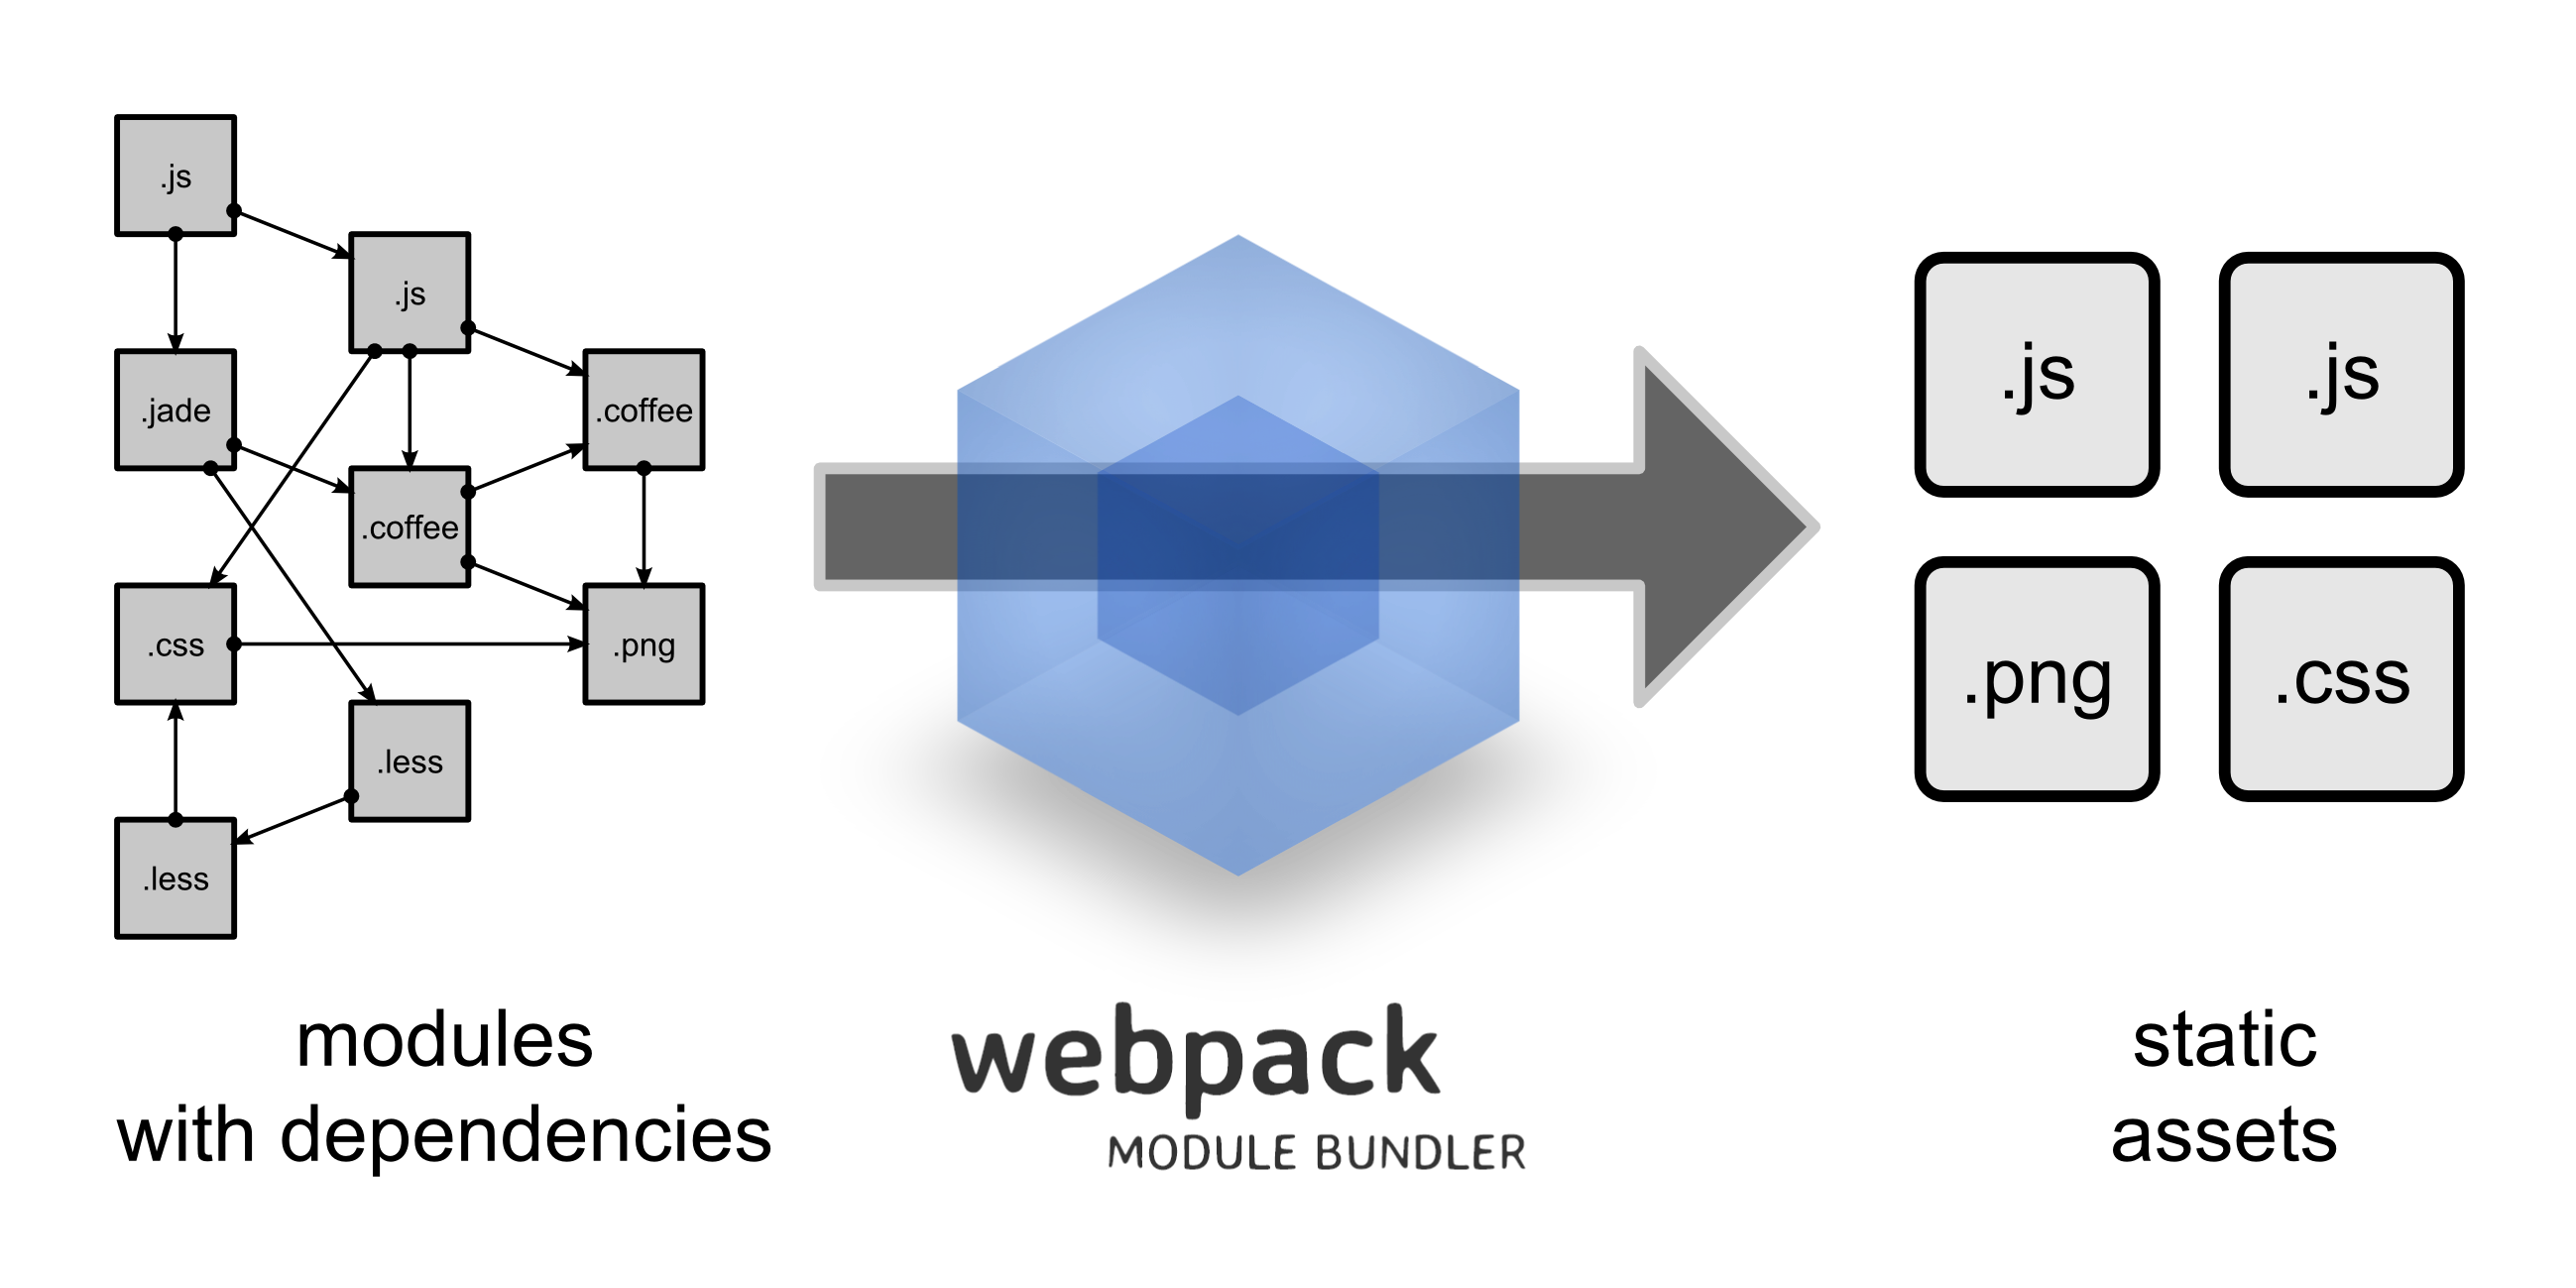
\includegraphics[width=\textwidth]{webpack.png}
    \caption{Zasada działania bundlera Webpack https://camo.githubusercontent.com/eac23581690c3ed7f73c0682aca8362fc0eff51ccd2700d28733f58936dd99d7/68747470733a2f2f7765627061636b2e6769746875622e696f2f6173736574732f776861742d69732d7765627061636b2e706e67}
    \label{fig:ast}
\end{figure}

W dużym projekcie proces ten potrafi być bardzo wolny. Razem z rozwojem ekosystemu JavaScript powstała opcja dynamicznych modułów ESM. Projektem realizującym ten mechanizm jest Vite. Dostarcza on rozwiązanie pozwalające budować i uruchamiać aplikacje Reactowe o wiele szybciej. Sprawa on, że kod, który aktualnie nie musi być używany, nie jest załadowany do pamięci - jest ładowany dynamicznie. Zasadniczym plusem takiego rozwiązania jest wsparcie dla HMR (Hot Module Reload) dzięki któremu w środowisku deweloperskim po wprowadzeniu drobnej zmiany nie jest konieczne ponowne zbundlowanie całego projektu, a tylko podmiana niewielkiego fragmentu kodu.

W tej części porównam czasy włączenia serwera deweloperskiego oraz zbudowania aplikacji.

Aplikację korzystającą z CRA stworzyłem korzystając z następujących komend:

\begin{lstlisting}[caption=Stworzenie i włączenie aplikacji React (CRA)]
npx create-react-app frontend-cra
cd frontend-cra
npm run start
\end{lstlisting}

Aplikację korzystającą z Vite stworzyłem używając: 

\begin{lstlisting}[caption=Stworzenie i włączenie aplikacji React (CRA)]
npm create vite@latest frontend-vite -- --template react-ts
cd frontend-vite
npm run dev
\end{lstlisting}

Obydwie aplikacje mają około 200 linijek kodu na starcie. W celu badania w drugim kroku rozszerzyłem je do około 10,000 linijek kodu. Poniższa zestawienie prezentuje czasy wykonywania poszczególnych operacji.

\begin{table}[H]
\centering
\begin{tabular}{|l|l|l|}
\hline
\textbf{Operacja} & \textbf{Liczba linijek} & \textbf{Czas wykonania (s)} \\ \hline
\multirow{2}{*}{Włączenia serwera deweloperskieogo} & 200 & 10 \\ 
& 10,000 & 39 \\ \hline
\multirow{2}{*}{Zbudowanie aplikacji} & 200 & 19 \\ 
& 10,000 & 50 \\ \hline
\end{tabular}
\caption{Czasy operacji dla CRA}
\label{tab:czas_wykonania}
\end{table}

\begin{table}[H]
\centering
\begin{tabular}{|l|l|l|}
\hline
\textbf{Operacja} & \textbf{Liczba linijek} & \textbf{Czas wykonania (s)} \\ \hline
\multirow{2}{*}{Włączenia serwera deweloperskieogo} & 200 & 2 \\ 
& 10,000 & 3 \\ \hline
\multirow{2}{*}{Zbudowanie aplikacji} & 200 & 5 \\ 
& 10,000 & 8 \\ \hline
\end{tabular}
\caption{Czasy operacji dla Vite}
\label{tab:czas_wykonania}
\end{table}


Poniżej czasy zestawione na wykresie:


\begin{figure}[H]
\centering
\begin{tikzpicture}
\begin{axis}[
    title={Porównanie czasów operacji dla CRA i Vite},
    xlabel={Liczba linijek},
    ylabel={Czas wykonania (s)},
    xmin=0, xmax=10500,
    ymin=0, ymax=55,
    xtick={200,10000},
    ytick={0,10,20,30,40,50},
    legend pos=north west,
    ymajorgrids=true,
    grid style=dashed,
    scaled y ticks=false,
    scaled x ticks=false,
]

\addplot[
    color=blue,
    mark=square,
    ]
    coordinates {
    (200,10)(10000,39)
    };
\addlegendentry{CRA - Włączenie serwera}

\addplot[
    color=blue,
    mark=triangle,
    ]
    coordinates {
    (200,19)(10000,50)
    };
\addlegendentry{CRA - Zbudowanie aplikacji}

\addplot[
    color=red,
    mark=square,
    ]
    coordinates {
    (200,2)(10000,3)
    };
\addlegendentry{Vite - Włączenie serwera}

\addplot[
    color=red,
    mark=triangle,
    ]
    coordinates {
    (200,5)(10000,8)
    };
\addlegendentry{Vite - Zbudowanie aplikacji}

\end{axis}
\end{tikzpicture}
\caption{Porównanie czasów operacji dla CRA i Vite}
\label{fig:cra_vs_vite}
\end{figure}

Jak widać, Vite oferuje niewiarygodne przyspieszenie czasu budowania. Co zdumiewające, nachylenie funkcji czasu wykonywania od liczby linijek jest bardzo niewielkie, co powoduje, że czym większy projekt, tym ta oszczędność staje się większa.

\subsection{Podsumowanie}

Powyższe badania udowadniają, że często domyślne zestawy narzędzi są dalekie od optymalnych. Optymalizację devops warto zacząć już od samego dobrania narzędzi najlepiej jeszcze przed rozpoczęciem projektu. Zmiany rozmiaru tych opisanych w powyższym rozdziale mogą być bardzo kosztowne w późniejszych fazach projektu.

\section{Metody wdrażania} \label{sectionMetodyWdrazania}

Po zbudowaniu aplikacji trzeba jej kod w jakiś sposób przenieść na serwer i na nim włączyć. Wypiszę teraz zarys sposobów, a w następnych działach każdy z nich opiszę dokładniej:

\begin{itemize}
    \item całkowicie ręczne wdrażanie na serwer - deweloper dostaje się na serwer, pobiera kod, instaluje potrzebne zależności i włącza na nim aplikację,
    \item ręczne wdrażanie z dodatkiem - deweloper nadal robi wszystko ręcznie, ale nad działaniem aplikacji czuwa pewien framework. Np. \textbf{Nodemon} do aplikacji NodeJS,
    \item manualna wirtualizacja - deweloper samodzielnie buduje obraz i wysyła go do repozytorium artefaktów. Następnie dostaje się do serwera i tam włącza obraz,
    \item automatyczna wirtuzalicja - istnieje proces, który po wprowadzeniu zmian automatycznie buduje obraz i wdraża go na serwer.
\end{itemize}

Wszystkie powyższe techniki zakładają, że deweloper ma dostęp do serwera poprzez SSH, a sam serwer jest uwierzytelniony do repozytorium kodu.

\subsection{Całkowicie ręczne wdrażanie}

Deweloper włącza manualnie aplikacje na serwerze. Musi podjąć większość kroków wykonywanych w środowisku lokalnym plus upewnić się, że serwer poprawnie obsługuje zapytania przychodzące z zewnątrz.

Szczególnie uciążliwa może być pierwsza konfiguracja. Należy w jej obrębie pobrać i skonfigurować narzędzia potrzebne do budowania i wdrażania aplikacji w danej technologii. W przypadku NodeJS będzie to npm. Dodatkowo może się okazać, że niektóre z zależności potrzebnych do działania aplikacji były zainstalowane globalnie na komputerze dewelopera, co spowoduje, że aplikacja nie zadziała i przysporzy to problemów natury debugowania.

\begin{figure}[H]
    \centering
    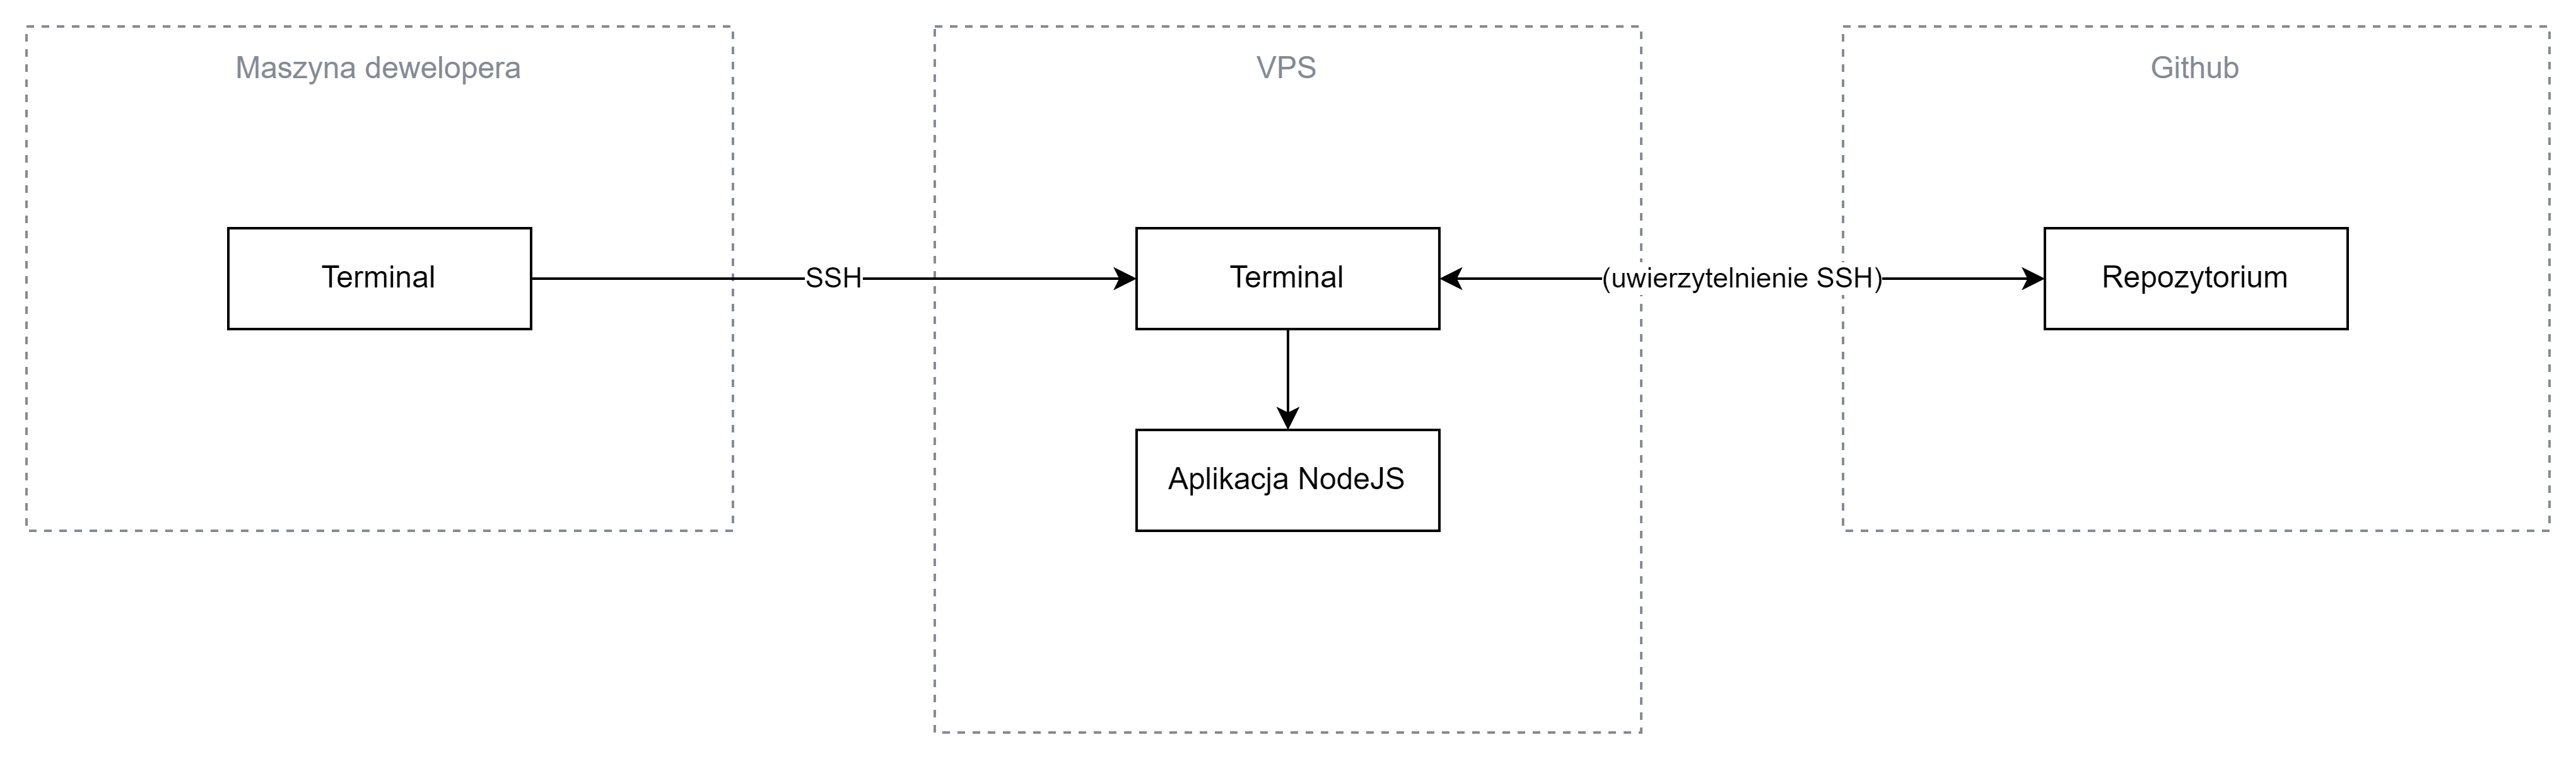
\includegraphics[width=1\linewidth]{reczne_wdrazanie.png}
    \caption{Całkowicie ręczne wdrażanie}
    \label{fig:enter-label}
\end{figure}

\begin{itemize}
    \item pobranie nowej wersji kodu,
    \item zainstalowanie potrzebnych zależności,
    \item zatrzymanie starej wersji aplikacji,
    \item włączenie nowej wersji aplikacji
\end{itemize}

\subsubsection{Zalety}

Metoda ta ma tylko jedną zaletę - czas. Pierwsze wdrożenie na serwer odbędzie się z pewnością szybciej. Nie ma potrzeby konfiguracji narzędzi automatyzujących pracę.

\subsubsection{Wady}

\begin{itemize}
    \item tracenie czasu na bardzo powtarzalne czynności przy każdym wdrożeniu,
    \item możliwość, że aplikacja nie będzie działać z uwagi na różnice w konfiguracji środowiska,
    \item brak możliwości dobrego monitorowania aplikacji,
    \item brak zarządzania stanem aplikacji (po restarcie serwera lub krytycznym błędzie w aplikacji pozostanie ona wyłączona),
    \item aplikacja ma bezpośredni dostęp do systemu operacyjnego hosta.
\end{itemize}

\subsection{Ręczne wdrażanie z dodatkiem}

Jako dodatek do ręcznego wdrożenia wybrałem Nodemon. Jest to narzędzie wprowadzające warstwę abstrakcji na aplikację NodeJS. Jest w stanie zarządzać stanem aplikacji - monitoruje, czy aplikacja jest "zdrowa". Dodatkowo pozwala na skalowanie aplikacji i zapewnia automatyczny load balancing. 

\begin{figure}[H]
    \centering
    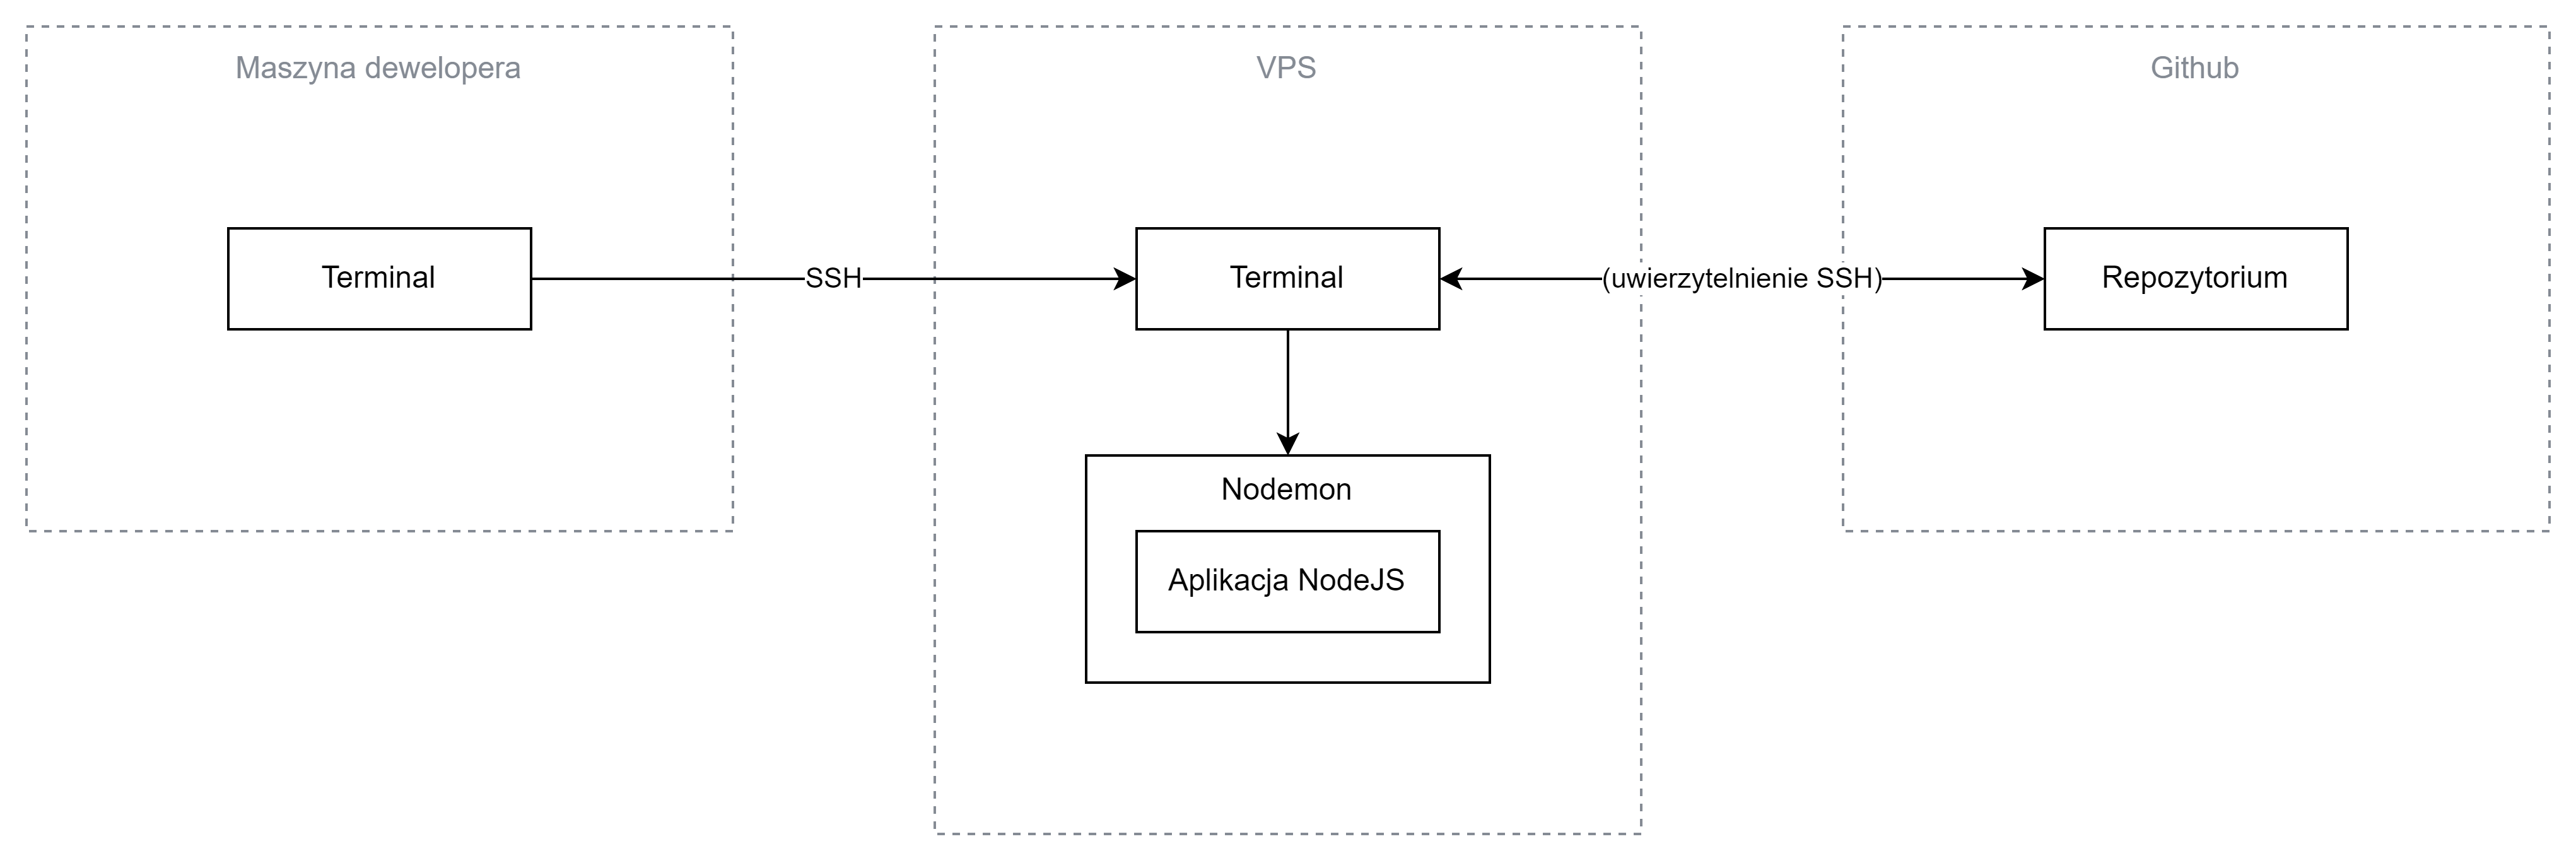
\includegraphics[width=1\linewidth]{reczneWdrazanieZDodatkiem.png}
    \caption{Ręczne wdrażanie z dodatkiem}
    \label{fig:enter-label}
\end{figure}

\subsubsection{Zalety}

\begin{itemize}
    \item podstawowe możliwości monitorowania aplikacji,
    \item zarządzanie stanem aplikacji (aplkacja sama się restartuje, jeżeli jest taka potrzeba),
    \item udostępnienie interfejsu do prostego skalowania aplikacji oraz automatycznego load balancera.
\end{itemize}

\subsubsection{Wady}

\begin{itemize}
    \item aplikacja nadal narażona jest na różnice w konfiguracji środowiska,
    \item aplikacja nadal ma bezpośredni dostęp do systemu operacyjnego hosta.
\end{itemize}

\subsection{Manualna wirtualizacja}

W tym przypadku deweloper buduje manualnie obraz na swoim komputerze i wysyła go do repozytorium artefaktów. Następnie dostaje się do maszyny, pobiera na niej obraz i włącza kontener z nową wersją aplikacji.

\begin{figure}[H]
    \centering
    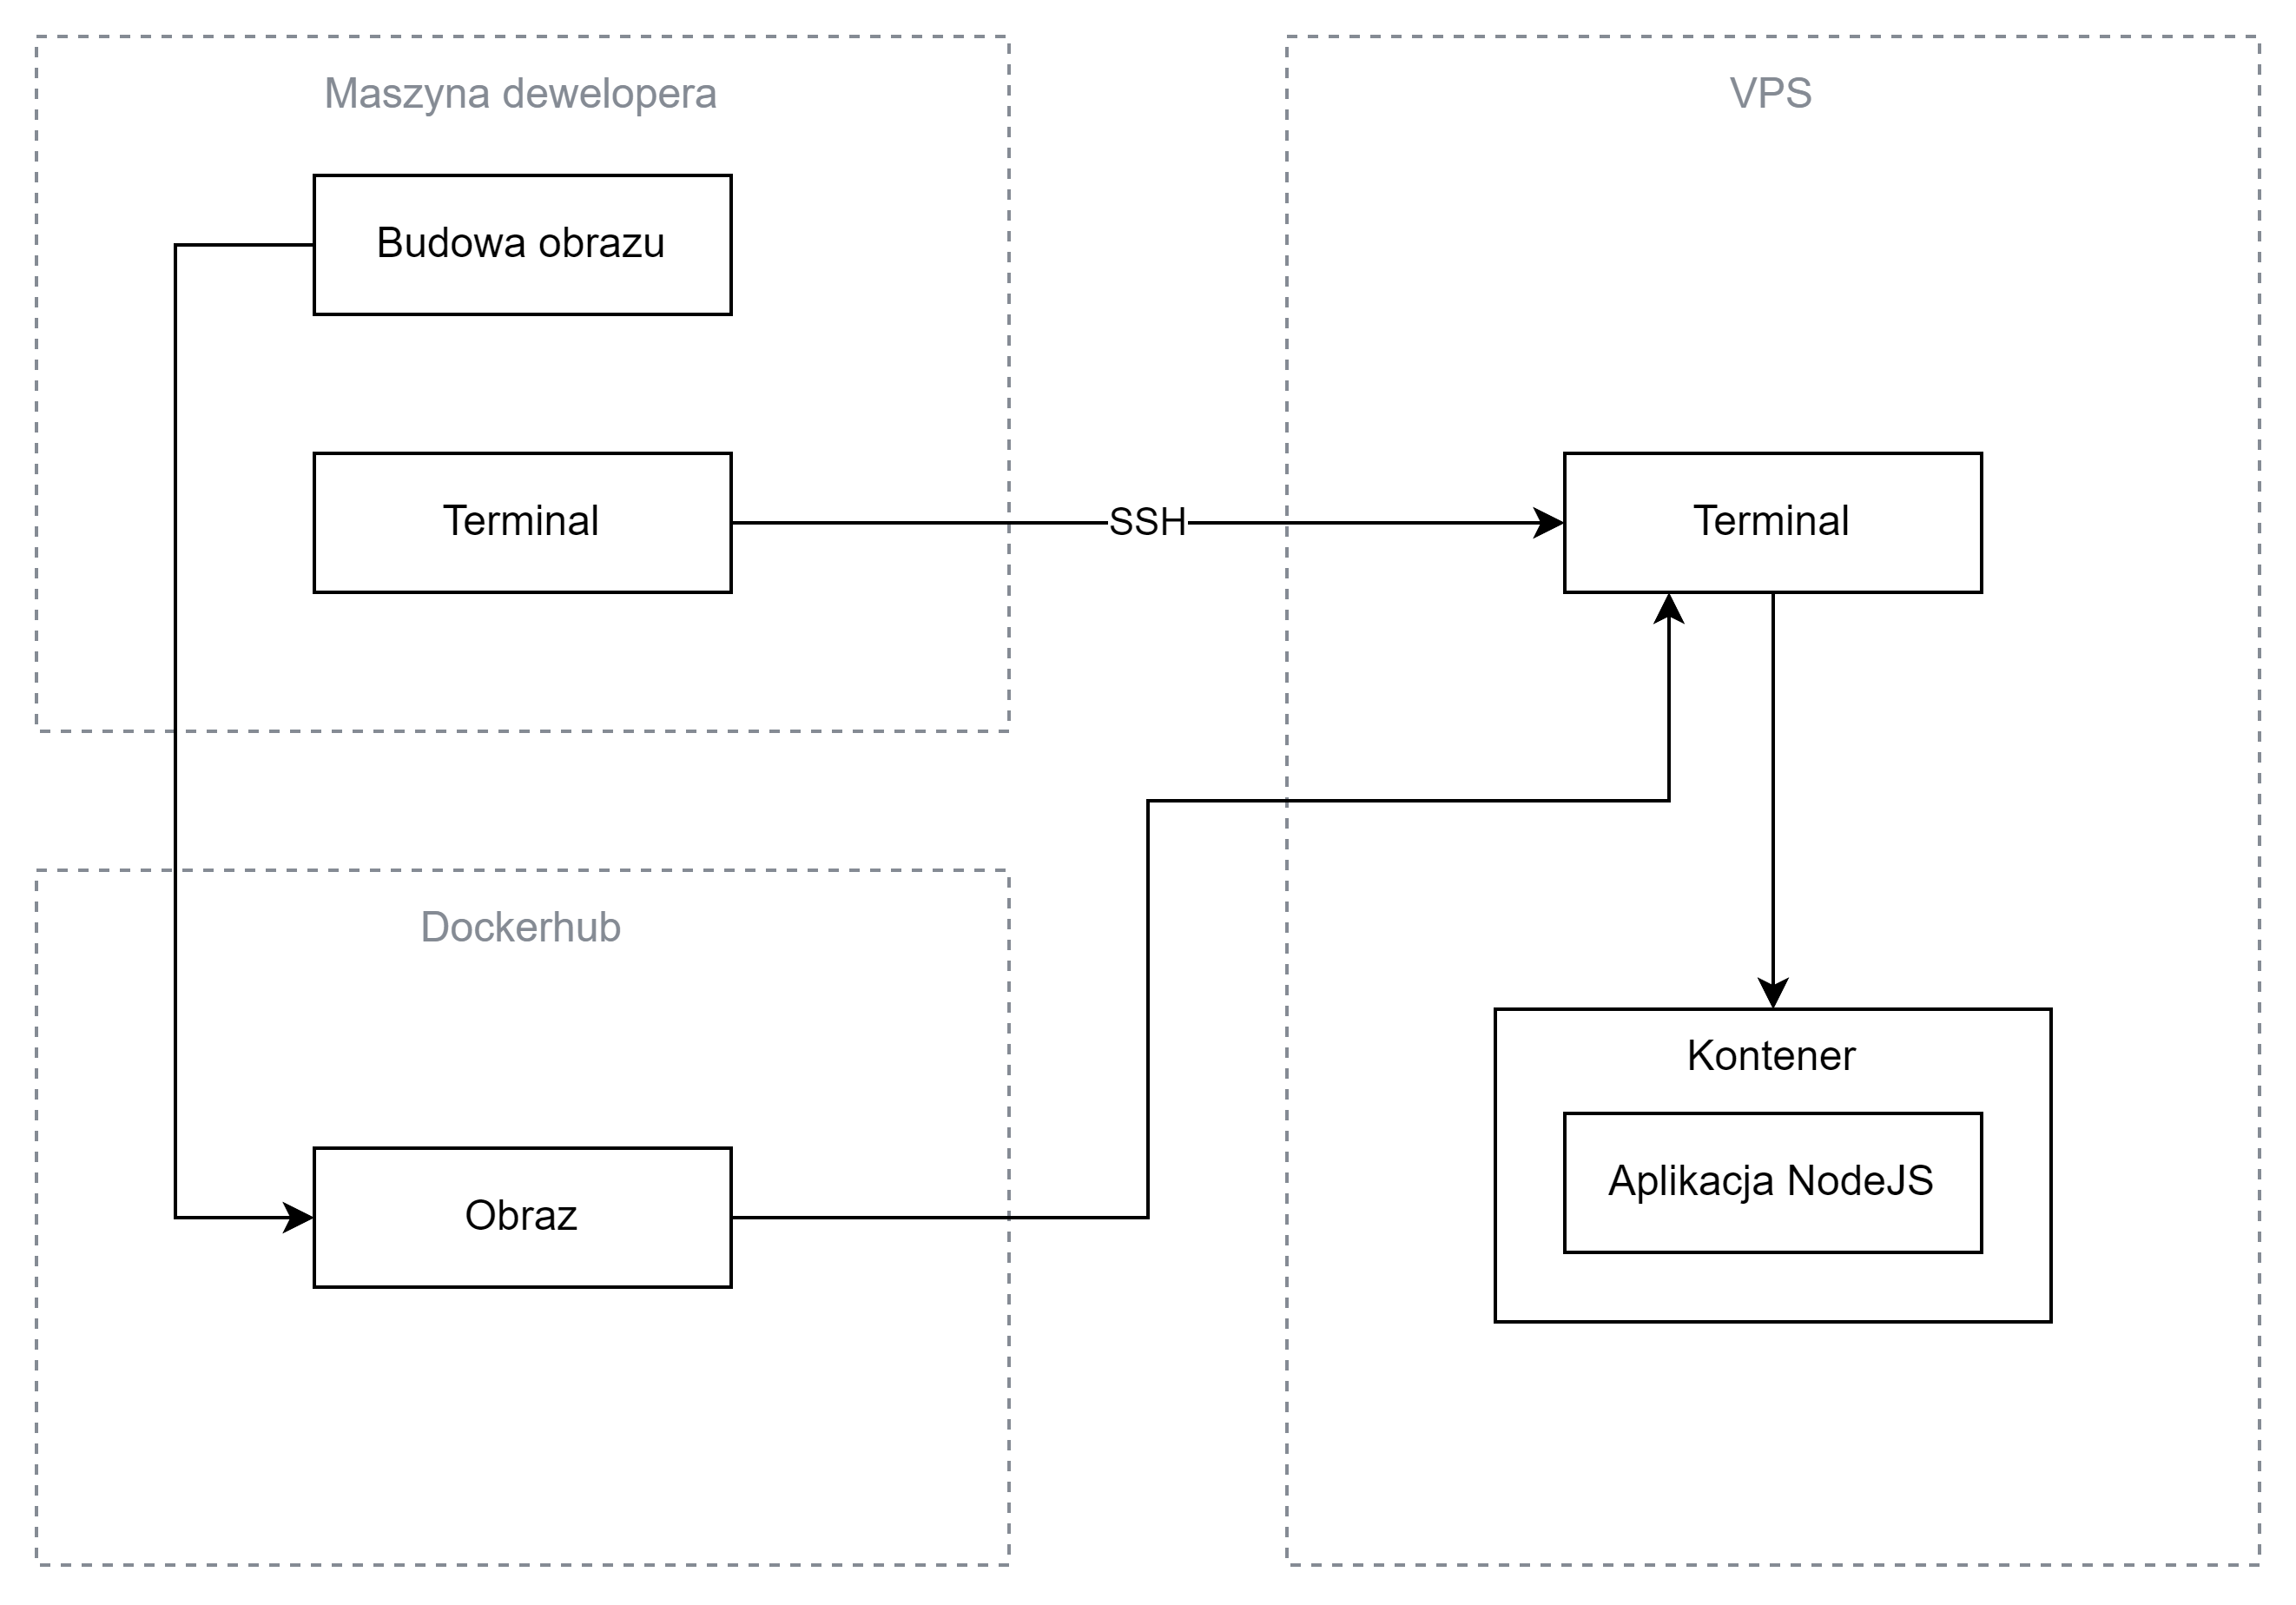
\includegraphics[width=1\linewidth]{manualnaWirtualizacja.png}
    \caption{Manualna wirtualizacja}
    \label{fig:enter-label}
\end{figure}

\subsubsection{Zalety}

\begin{itemize}
    \item o wiele szybsza konfiguracja środowiska. Na serwerze musi być tylko zainstalowany narzędzie obsługujące wirtualizację,
    \item drastycznie zredukowana szansa wystąpienia błędów w wyniku różnic w konfiguracji. Deweloper może obraz najpierw przetestować na swojej lokalnej maszynie,
    \item aplikacja nie ma dostępu do systemu operacyjnego hosta.
\end{itemize}

\subsubsection{Wady}

\begin{itemize}
    \item znaczne skomplikowanie infrastruktury projektu. Od teraz trzeba utrzymywać repozytorium obrazów,
    \item utrudnienie zmian w konfiguracji aplikacji. Możliwe, że zwykły deweloper nie będzie potrafił wprowadzić zmian obejmujących rzeczy poza samym kodem do aplikacji,
\end{itemize}

\subsection{Wirtualizacja + CI/CD}

W tym podejściu deweloper buduje infrastrukturę CI/CD umożliwiając całkowicie automatyczne wdrażanie aplikacji. Po wgraniu do repozytorium kodu zmian, agent automatycznie się uruchamia, buduje obraz, a następnie dostaje się do serwera i na nim włącza kontener

\begin{figure}[H]
    \centering
    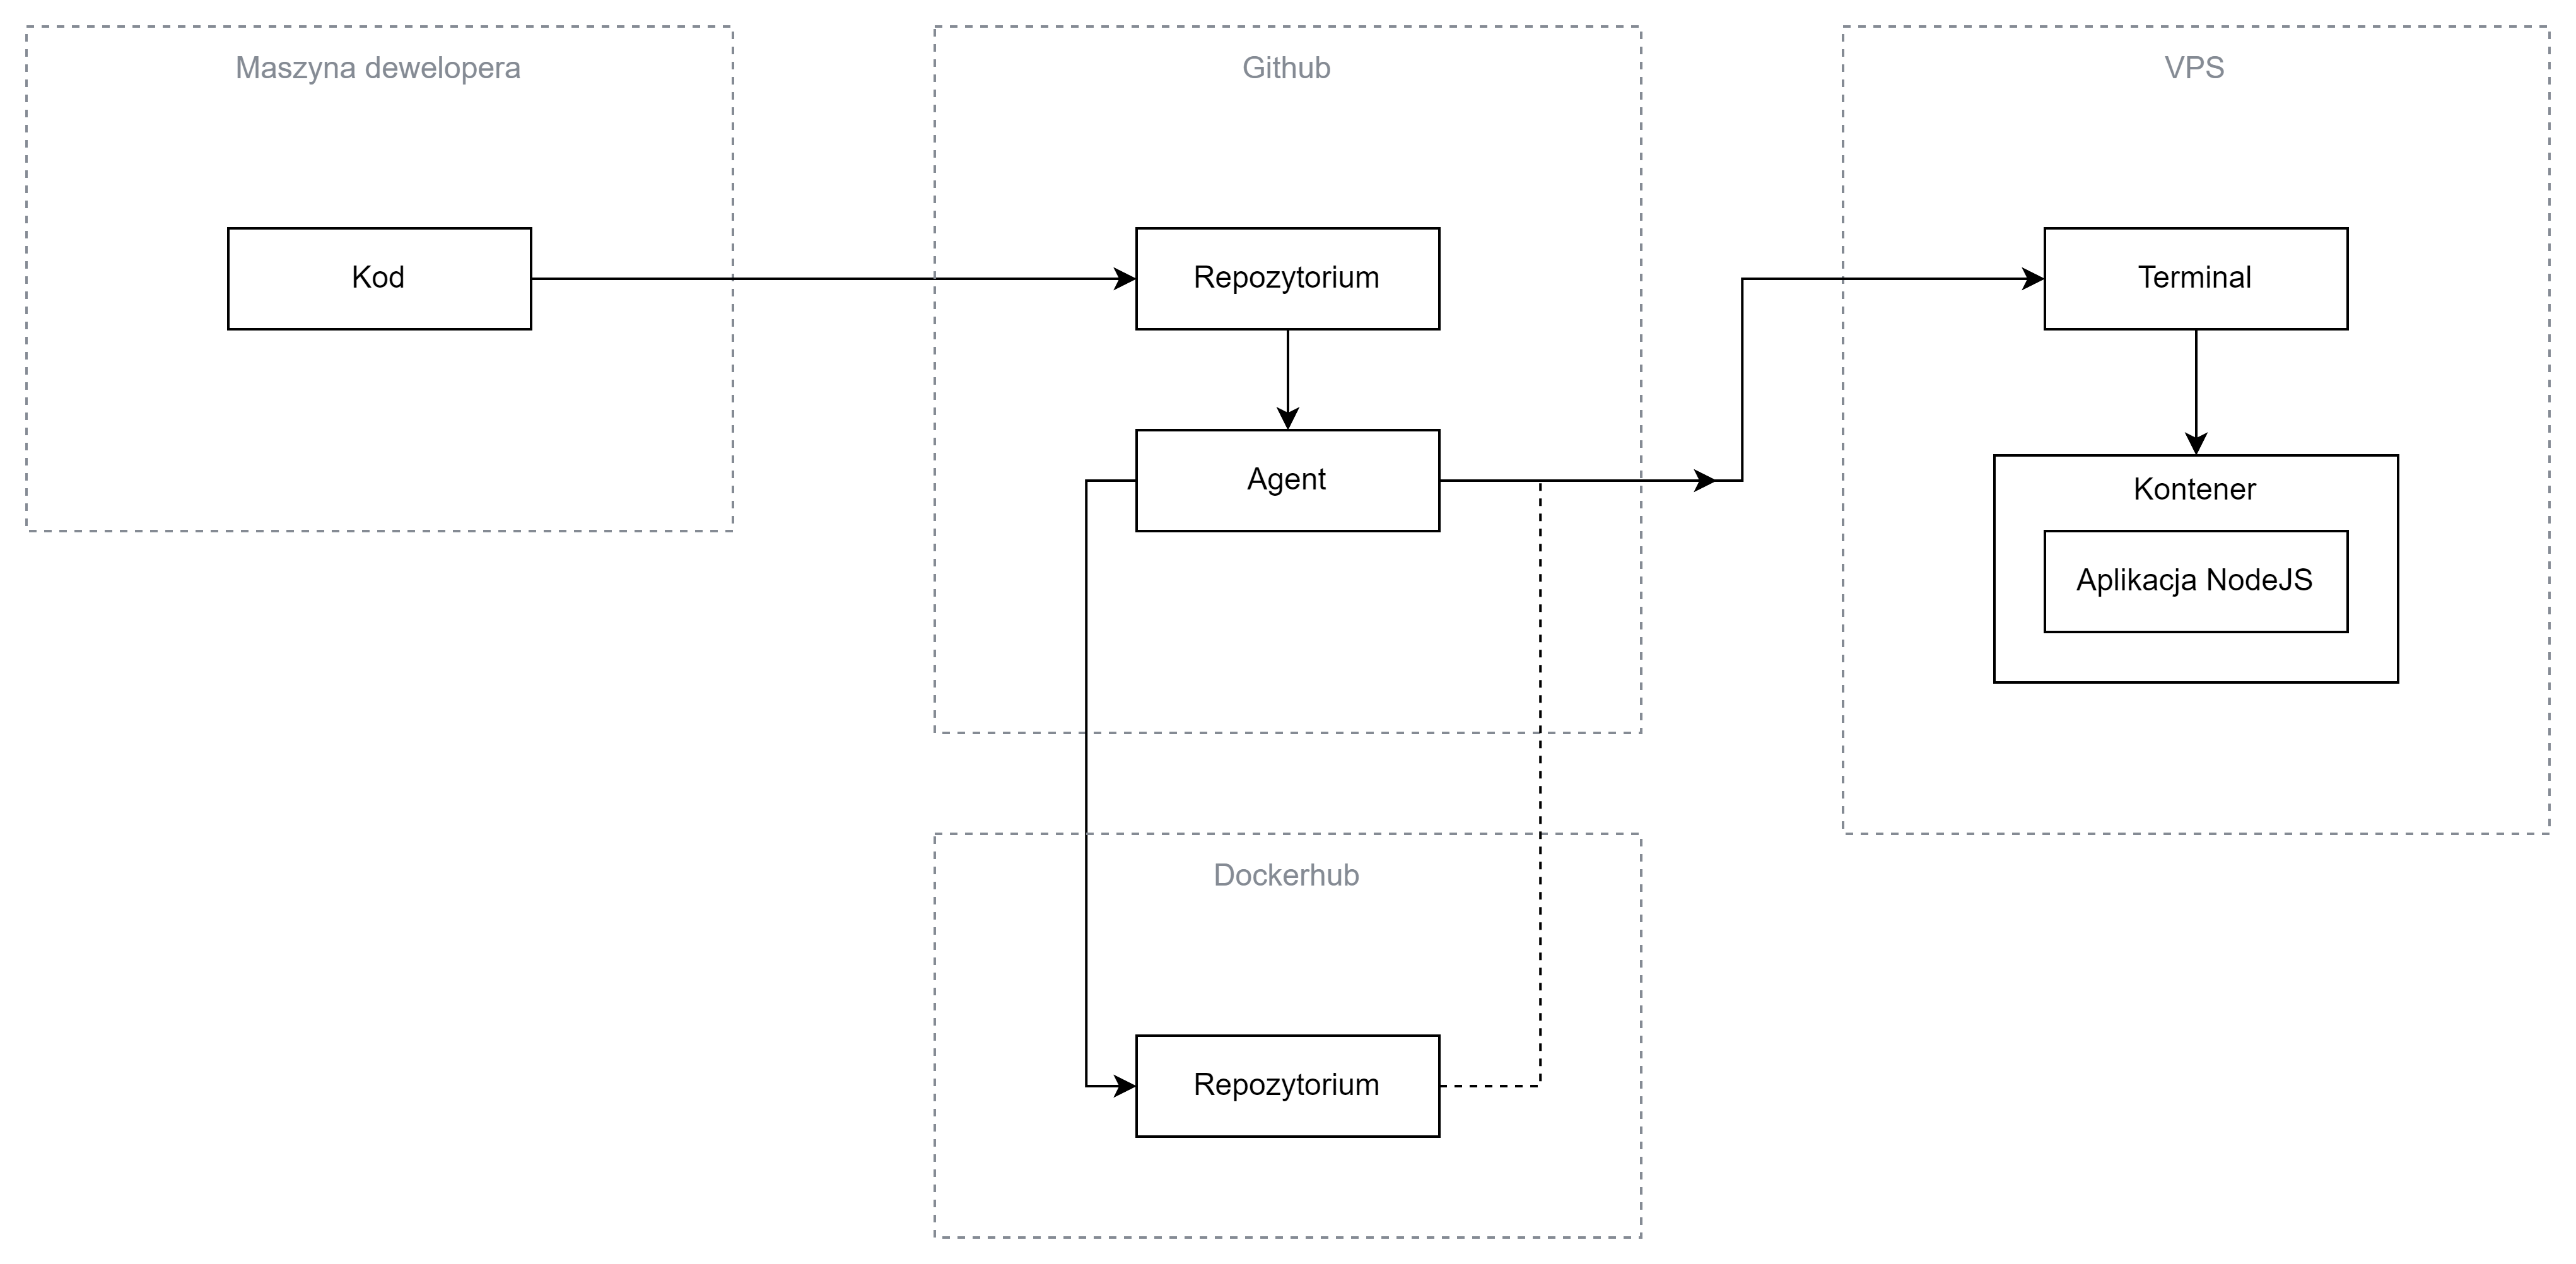
\includegraphics[width=1\linewidth]{automatycznaWirtualizacja.png}
    \caption{Wirtualizacja + CI/CD}
    \label{fig:enter-label}
\end{figure}

\subsubsection{Zalety}

\begin{itemize}
    \item znaczące usprawnienie procesu wdrażania aplikacji,
    \item minimalizacja błędów konfiguracji,
    \item bardzo łatwe rozszerzenie na kilka środowisk.
\end{itemize}

\subsubsection{Wady}

\begin{itemize}
    \item znaczne skomplikowanie infrastruktury projektu. Potrzeba wybrania narzędzia do CI/CD oraz tworzenia i utrzymywania plików konfiguracyjnych,
\end{itemize}

\subsection{Podsumowanie}

\begin{table}[H]
\centering
\begin{tabular}{|l|c|c|c|c|}
\hline
\textbf{Cecha} & \textbf{1} & \textbf{2} & \textbf{3} & \textbf{4} \\ \hline
Podatność na błędy konfiguracji         & \cellcolor{red!50}wysoka & \cellcolor{red!50}wysoka & \cellcolor{green!50}niska & \cellcolor{green!50}niska \\ \hline
Czas potrzebny na pierwszą konfigurację & \cellcolor{green!50}niski & \cellcolor{yellow!50}średni & \cellcolor{red!50}wysoki & \cellcolor{red!50}bardzo wysoki \\ \hline
Czas wdrożenia nowej wersji aplikacji   & \cellcolor{red!50}wysoki & \cellcolor{red!50}wysoki & \cellcolor{yellow!50}średni & \cellcolor{green!50}niski \\ \hline
Zarządzanie stanem aplikacji            & \cellcolor{red!50}nie & \cellcolor{green!50}tak & \cellcolor{green!50}tak & \cellcolor{green!50}tak \\ \hline
Skalowanie aplikacji                    & \cellcolor{red!50}trudne & \cellcolor{green!50}łatwe & \cellcolor{green!50}łatwe & \cellcolor{green!50}łatwe \\ \hline
Podatność na ataki                      & \cellcolor{red!50}wysoka & \cellcolor{red!50}wysoka & \cellcolor{green!50}niska & \cellcolor{green!50}niska \\ \hline
Monitorowanie aplikacji                 & \cellcolor{red!50}nie & \cellcolor{red!50}nie & \cellcolor{green!50}tak & \cellcolor{green!50}tak \\ \hline
\end{tabular}
\caption{Porównanie metod wdrażania: 1 - całkowicie ręczne, 2 - ręczne z dodatkiem, 3 - wirtualizacja, 4 - wirtualizacja + CI/CD}
\label{tab:porownanie-metod-wdrazania}
\end{table}

Zasadniczym plusem ręcznego wdrażania jest szybkość pierwszej konfiguracji. Nie trzeba konfigurować praktycznie nic, tylko włączyć aplikację na serwerze. Uważam jednak, że liczba zalet wirtualizacji z użyciem CI/CD przewyższa zysk czasowy manualnego wdrażania. Warto poświęcić na początku więcej czasu na dobrą konfigurację aby zaoszczędzić go w późniejszych fazach rozwoju aplikacji.


\section{Budowa obrazu} \label{sectionBudowaObrazu}

\subsection{Podstawowy obraz}

Zacznę od przeanalizowania najprostszego obrazu dockerowego, aby aplikacja po prostu działała. W tym celu dodałem do folderu z aplikacją plik \textbf{Dockerfile} o następującej treści

\begin{lstlisting}[caption=Podstawowy plik Dockerfile]
FROM node:18

WORKDIR /usr/src/app

COPY package*.json ./

RUN npm install

COPY . .

RUN npm run build

CMD [ "node", "dist/main.js" ]
\end{lstlisting}

Z definicji pliku wynika, że wybiera on obraz bazowy, przenosi pliki konfiguracyjne, instaluje potrzebne zależności, przenosi pliki źródłowe, buduje aplikacje i ją włącza.

Czas potrzebny na zbudowanie obrazu to \textbf{85 sekund}. Rozmiar obrazu to \textbf{1.64GB}. Warto zwrócić uwagę na to, który krok zajął najwięcej czasu. Był to krok \lstinline|[internal] load build context|.

\subsection{Dockerignore}

Warto wiedzieć, że NodeJS potrzebne zależności przechowuje w folderze, w którym znajdują się pliki projektu. Oznacza to, że instrukcja \lstinline|COPY . .| z pliku Dockerfile przeniesie je wszystkie do obrazu, co nie jest konieczne, ponieważ w obrazie i tak trzeba je pobrać.

W takim celu używa się pliku \lstinline|.dockerignore|, w którym podaje się listę rzeczy, które Docker ma ignorować podczas instrukcji kopiowania

\begin{lstlisting}[caption=Plik .dockerignore]
dist
node_modules
\end{lstlisting}

Oprocz folderu z zależnościami dobrze nie przenosić również folderu ze zbudowaną aplikacją, ponieważ ta i tak musi się zbudować ponownie w obrazie

Po wprowadzeniu pliku \lstinline|.dockerignore| proces zajmuje teraz \textbf{24 sekundy}, a rozmiar zbudowanego obrazu to \textbf{1.42GB}.

\subsection{Multi stage build}

Node dzieli swoje zależności na standardowe i deweloperskie. Standardowe to te, które są potrzebne do tego, żeby aplikacja działała. Deweloperskie natomiast to takie, które są potrzebne tylko w momencie budowania aplikacji.

Dobrym przykładem zależności deweloperskiej jest \textbf{Typescript}. Jest to paczka, która zawiera definicje potrzebne do przetłumaczenia Typescript na Javascript, ale po przetłumaczeniu nie jest już potrzebna,

\begin{lstlisting}[caption=Multistage plik Dockerfile]
FROM node:18 AS development
WORKDIR /usr/src/app
COPY package*.json ./
RUN npm ci -f
COPY . .


FROM node:18 AS build
WORKDIR /usr/src/app
COPY package*.json ./
COPY --from=development /usr/src/app/node_modules ./node_modules
COPY . .
RUN npm run build
RUN npm ci -f --only=production && npm cache clean --force


FROM node:18 AS production
ENV NODE_ENV production
COPY --from=build /usr/src/app/node_modules ./node_modules
COPY --from=build /usr/src/app/dist ./dist
CMD [ "node", "dist/main.js" ]
\end{lstlisting}

Wylistowany wyżej plik \lstinline|Dockerfile| stosuje 3 etapowy proces budowania.

\begin{enumerate}
    \item development - ta część odpowiedzialna jest za zainstalowanie zależności i skopiowanie plików źródłowych do obrazu,
    \item build - ta część kopiuje zależności, które pobrał pierwszy krok, buduje aplikacje, a następnie wywołuje komendę \lstinline|npm ci -f --only=production && npm cache clean --force|, która nadpisuje zależności w taki sposób, że zostaną tylko te wymagane do poprawnego działania aplikacji (zignoruje zależności deweloperskie,
    \item production - ostatni krok kopiuje potrzebne zależności oraz kod źródłowy i włącza aplikację
\end{enumerate}

Ta konfiguracja zajmuje \textbf{30 sekund}, a rozmiar zbudowanego obrazu to \textbf{1.09GB}

\subsection{Alpine}

Dotychczas korzystałem z obrazu bazowego \lstinline|node:18|. Jest on całkiem spory, ponieważ zawiera pełną dystrubucję linuxa. W przypadku tej (i zdecydowanej większości) aplikacji nie jest potrzebne większość narzędzi z oficjalnej dystrybucji linuxa. 

Można w tym celu użyć dystrybucji typu \textbf{alpine}. Nazwa obrazu to wtedy \lstinline|node:18-alpine|.

W tej konfiguracji obraz buduje się \textbf{33 sekundy} i zajmuje \textbf{148MB} miejsca.

\subsection{Distroless}

Działania opisane w poprzednich krokach miały na celu przyspieszenie procesu budowania lub zmniejszenie rozmiaru obrazu. Istnieje jednak pewna praktyka, którą stosuje się w celu zwiększenie bezpieczeństwa aplikacji.

Sama wirtualizacja zapewnia to, że jeżeli atakujący dostanie się na maszynę, na której włączona jest aplikacja, to nie ma dostępu do systemu operacyjnego hosta, tylko jest "zamknięty" w kontenerze. Ogranicza to znacząco liczbę niechcianych rzeczy, które może zrobić, ale jednak wciąż może coś wykraść z wewnątrz kontenera lub wysłać jakieś requesty sieciowe.

Istnieje odmiana obrazów nazywana \textbf{distroless} i charakteryzuje się ona tym, że taki obraz nie posiada warstwy \textbf{shell}. Nie da się na nic wywołać żadnych komend. Nie da się użyć tego obrazu w dwóch pierwszych krokach budowania, ponieważ tam wywoływane są jakieś komendy \lstinline|RUN|. Używa się go tylko w ostatnim kroku budowy, usuwając jednocześnie \lstinline|node| z polecenia \lstinline|CMD|. 

\begin{lstlisting}[caption=Ostatni etap distroless Dockerfile]
FROM gcr.io/distroless/nodejs18-debian12 AS production
ENV NODE_ENV production
COPY --from=build /usr/src/app/node_modules ./node_modules
COPY --from=build /usr/src/app/dist ./dist
CMD [ "dist/main.js" ]
\end{lstlisting}

Taki obraz buduje się \textbf{34 sekundy}, zajmuje \textbf{175MB} miejsca, ale jest bardzo bezpieczny.

\subsection{Cache}

Na potrzeby wyżej przeprowadzonych badań używałem komendy budującej obraz z argumentem \lstinline|--no-cache|. W rzeczywistych warunkach się tego nie robi. Docker sprytnie cachuje warstwy, przez co powtarzalne kroki nie muszą zostać ponownie wywołane. Głównie czas oszczędza się na instalowaniu zależności. Nowe zależności zostaną pobrane tylko wtedy, gdy zmieni się zawartość pliku \lstinline|package.json| lub \lstinline|package-lock.json|.

W przypadku użycia cache obraz buduje się około 5 sekund.

\newpage

\subsection{Podsumowanie}

Z początkowego 1.64GB udało się zejść do 175MB, przy tym samym przyspieszając budowę 3 krotnie. Dodatkowo użycie obrazu distroless sprawiło, że aplikacja jest o wiele bardziej bezpieczna.


\begin{figure}[H]
\centering
\begin{tikzpicture}
\begin{axis}[
    width=\textwidth/1.2,
    height=200,
    ybar,
    bar width=0.6cm,
    enlarge x limits=0.1,
    ylabel={Czas (s)}, 
    symbolic x coords={Podstawowy,Dockerignore,Multistage,Alpine,Distroless},
    xtick=data,
    nodes near coords,
    nodes near coords align={vertical},
    ]
    \addplot[blue,fill=blue] coordinates {(Podstawowy,85) (Dockerignore,24) (Multistage,30) (Alpine,33) (Distroless,34)};
\end{axis}
\end{tikzpicture}
\caption{Porównanie czasu budowania obrazu}
\label{fig:czas}
\end{figure}

\begin{figure}[H]
\centering
\begin{tikzpicture}
\begin{axis}[
    width=\textwidth/1.2,
    height=200,
    ybar,
    bar width=0.6cm,
    enlarge x limits=0.1,
    ylabel={Miejsce (GB)},
    symbolic x coords={Podstawowy,Dockerignore,Multistage,Alpine,Distroless},
    xtick=data,
    nodes near coords,
    nodes near coords align={vertical},
    ]
    \addplot[red,fill=red] coordinates {(Podstawowy,1.64) (Dockerignore,1.42) (Multistage,1.09) (Alpine,0.148) (Distroless,0.175)};
\end{axis}
\end{tikzpicture}
\caption{Porównanie zajętego miejsca przez obrazy}
\label{fig:miejsce}
\end{figure}

\section{CI/CD} \label{sectionCICD}

\subsection{Wprowadzenie}

\subsubsection{Cel}

Zadaniem CI/CD jest zautomatyzowanie czynności związanych z testowaniem, budowaniem i wdrażaniem aplikacji. Chcemy osiągnąć ciągłość integracji (Continuous Integration) oraz ciągłość dostarczania (Continuous Delivery/Deployment), co pozwoli na:

\begin{itemize}
\item Automatyczne uruchamianie testów jednostkowych i integracyjnych po każdym commitcie, co zapewnia wczesne wykrywanie błędów.
\item Automatyczne budowanie aplikacji po każdym commitcie, co umożliwia szybsze wdrażanie nowych wersji.
\item Automatyczne wdrażanie aplikacji na środowiska testowe i produkcyjne, co przyspiesza proces wydawania nowych wersji i minimalizuje ryzyko błędów wynikających z ręcznego wdrażania.
\item Zapewnienie spójności środowisk poprzez zautomatyzowane procesy budowania i wdrażania.
\item Zwiększenie produktywności zespołu poprzez automatyzację powtarzalnych zadań.
\end{itemize}

\subsubsection{Wybór platformy}

Najpopularniejszą platformą i oferującą jednocześnie najwięcej opcji jest z pewnością Gitlab, ale wymaga bardzo czasochłonnej konfiguracji jeszcze przed samym zaczęciem konfiguracji CI/CD.

Ja jako platformę CI/CD wybrałem \textbf{Github Actions}, ponieważ jest darmowa dla publicznych projektów, bardzo dobrze udokumentowana i nie wymaga żadnej początkowej konfiguracji. Językiem opisu są tutaj pliki \lstinline|.yml| mieszczone w folderze \lstinline|.github| w głównym folderze projektu.

\subsection{Pojęcia}

\subsubsection{Pipeline}

Pipeline CI/CD składa się z serii kroków, które są wykonywane automatycznie po każdym commitcie. W przypadku Github Actions, konfiguracja pipeline'u odbywa się za pomocą plików YAML, które definiują kroki, jakie mają być wykonane. Poniżej przedstawiam przykładowy pipeline

\begin{lstlisting}[caption=Przykładowa konfiguracja pipeline'u w Github Actions]
name: CI/CD Pipeline

on:
push:
  branches:
    - main

jobs:
  example:
    runs-on: ubuntu-latest

steps:
- name: Print hello world
  run: echo "Hello world"

\end{lstlisting}

Pipeline składa się z sekcji konfiguracyjnej, w której wyspecyfikowane jest, co ma go włączać. W tym przypadku jest to akcja push na branch main.

W następnej sekcji zdefiniowane jest, jakiego typu agent zostanie przydzielony. W tym wypadku jest to ubuntu.

W ostatniej sekcji zdefiniowane są kroki pipeline. Tutaj włączany jest tylko jeden krok, który wywołuje komendę bezpośrednio na agencie, która wypisze na ekran "Hello world"

\subsubsection{Agent}

W kontekście CI/CD, agent jest to bezstanowa maszyna wirtualna lub kontener, na którym wykonywane są kroki zdefiniowane w pipeline. Agent jest odpowiedzialny za wykonanie zadań takich jak budowanie, testowanie i wdrażanie aplikacji. W Github Actions, agentem jest maszyna uruchomiona przez Github, na której uruchamiane są kroki zdefiniowane w pliku YAML.

Agent jest kluczowym elementem w procesie CI/CD, ponieważ to na nim wykonywane są wszystkie operacje, które składają się na cały proces. Każdy job w pipeline jest uruchamiany na oddzielnym agencie, co pozwala na równoległe wykonywanie zadań i zwiększa efektywność procesu. Agenty są bezstanowe, co oznacza, że każde uruchomienie joba zaczyna się od nowej, czystej maszyny, co minimalizuje ryzyko wystąpienia problemów wynikających z zależności między zadaniami.


\subsubsection{Gotowe akcje GitHub Actions}

Jedną z zalet korzystania z GitHub Actions jest dostępność gotowych akcji (actions), które upraszczają i przyspieszają konfigurację pipeline'ów CI/CD. Akcje te są predefiniowanymi, wielokrotnego użytku fragmentami kodu, które można łatwo zintegrować z własnym pipeline'em. Dzięki nim, można nałożyć abstrakcję na powtarzalne i skomplikowane zadania, co znacząco upraszcza proces automatyzacji.

Gotowe akcje można znaleźć w oficjalnym GitHub Marketplace, gdzie dostępne są tysiące akcji przygotowanych przez społeczność oraz samych twórców GitHub. Akcje te mogą obejmować różnorodne zadania, takie jak:

\begin{itemize}
\item Analiza kodu: Integracja z narzędziami do analizy statycznej kodu, linterami oraz sprawdzanie jakości kodu.
\item Bezpieczeństwo: Automatyczne skanowanie kodu w poszukiwaniu podatności, zarządzanie sekretami oraz zapewnienie zgodności z politykami bezpieczeństwa.
\item Wdrażanie: Akcje do wdrażania aplikacji na różne środowiska, w tym na serwery, usługi chmurowe (np. AWS, Azure, Google Cloud) oraz platformy kontenerowe (np. Docker, Kubernetes).
\item Powiadomienia: Integracja z narzędziami do komunikacji i zarządzania projektem, takimi jak Slack, Microsoft Teams, czy e-mail, w celu wysyłania powiadomień o stanie pipeline'u.
\end{itemize}

Korzystanie z gotowych akcji pozwala na znaczące zmniejszenie ilości kodu konfiguracyjnego oraz eliminację potencjalnych błędów wynikających z ręcznego definiowania skomplikowanych kroków. Na przykład, zamiast samodzielnie pisać skrypty do instalacji zależności i uruchamiania testów, można skorzystać z gotowych akcji, takich jak \lstinline|actions/setup-node| dla Node.js czy \lstinline|actions/checkout| do pobierania kodu źródłowego.

\subsubsection{Sekrety}

Sekrety w kontekście CI/CD to poufne informacje, takie jak klucze API, dane logowania, tokeny dostępu czy hasła, które są niezbędne do działania różnych etapów pipeline'u, ale które nie powinny być ujawniane publicznie. Wiele platform CI/CD, takich jak Github Actions, Gitlab CI czy Jenkins, umożliwia przechowywanie i zarządzanie sekretami w bezpieczny sposób.

Mimo że pliki konfiguracyjne pipeline'ów mogą być publiczne, same sekrety są ukryte i niedostępne dla osób postronnych. Nawet gdy pipeline jest otwarty dla publicznego wglądu, wartości sekretów pozostają niewidoczne. Sekrety są wstrzykiwane do pipeline'u jako zmienne środowiskowe tylko w momencie wykonywania pipeline'u, co zapewnia ich bezpieczeństwo. W publicznym do wglądu logu pipeline wyświetlane są tak:

\begin{figure}[H]
    \centering
    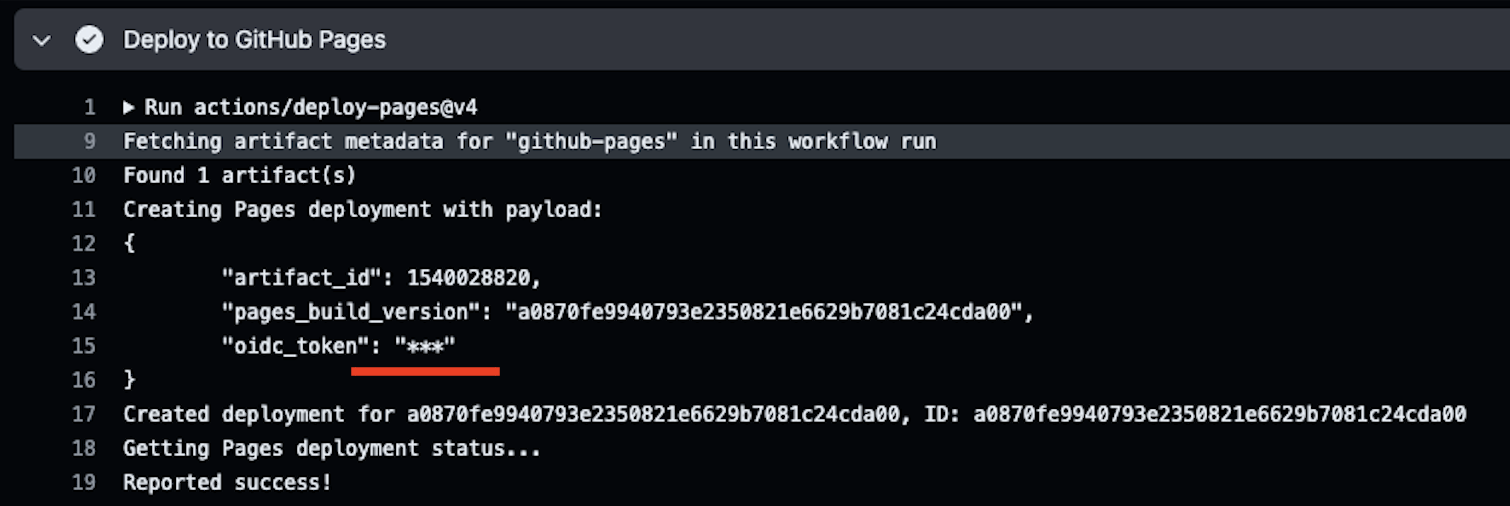
\includegraphics[width=1\linewidth]{actionsLogSecrets.png}
    \caption{Przykład wyświetlania wartości sekretu w logach pipeline}
    \label{fig:enter-label}
\end{figure}

Na przykład w Github Actions, sekrety można skonfigurować w ustawieniach repozytorium:

\begin{enumerate}
\item Przejdź do sekcji "Settings" w swoim repozytorium.
\item Wybierz "Secrets and variables" z menu po lewej stronie.
\item Kliknij "New repository secret", aby dodać nowy sekret.
\end{enumerate}

Po dodaniu sekrety można używać w plikach YAML definiujących pipeline, w ten sposób

\begin{lstlisting}[caption=Przykładowa konfiguracja pipeline'u w Github Actions]
- value: ${{ secrets.MY_SECRET }}
\end{lstlisting}

\subsection{Najlepsze praktyki}
Pisanie dobrych pipelinów ma zasady bardzo podobne do zasad pisania czystego kodu. Przytoczę kilka z nich

\subsubsection{Odpowiedzialność}

Każda akcja w pipeline CI/CD powinna spełniać zasadę pojedynczej odpowiedzialności, czyli wykonywać tylko jedno, dobrze zdefiniowane zadanie. Unikanie dużych, złożonych plików konfiguracyjnych, które realizują wszystkie kroki procesu, jest kluczowe dla utrzymania przejrzystości i łatwości zarządzania. Dzięki temu podejściu, można również uruchamiać wiele akcji równocześnie tam, gdzie to możliwe, co zwiększa efektywność i skraca czas wykonania całego pipeline'u.

Przykładowy proces budowania aplikacji może obejmować kroki takie jak:

\begin{itemize}
    \item zbudowanie,
    \item przetestowanie,
    \item analiza kodu sonarqube
\end{itemize}

Zakładając, że wszystkie te kroki opisane są w jednej akcji i że każda z czynności zajmuje 1 jednostkę czasu, to cały pipeline wykona się w 3 jednostki czasu.

\begin{figure}[H]
    \centering
    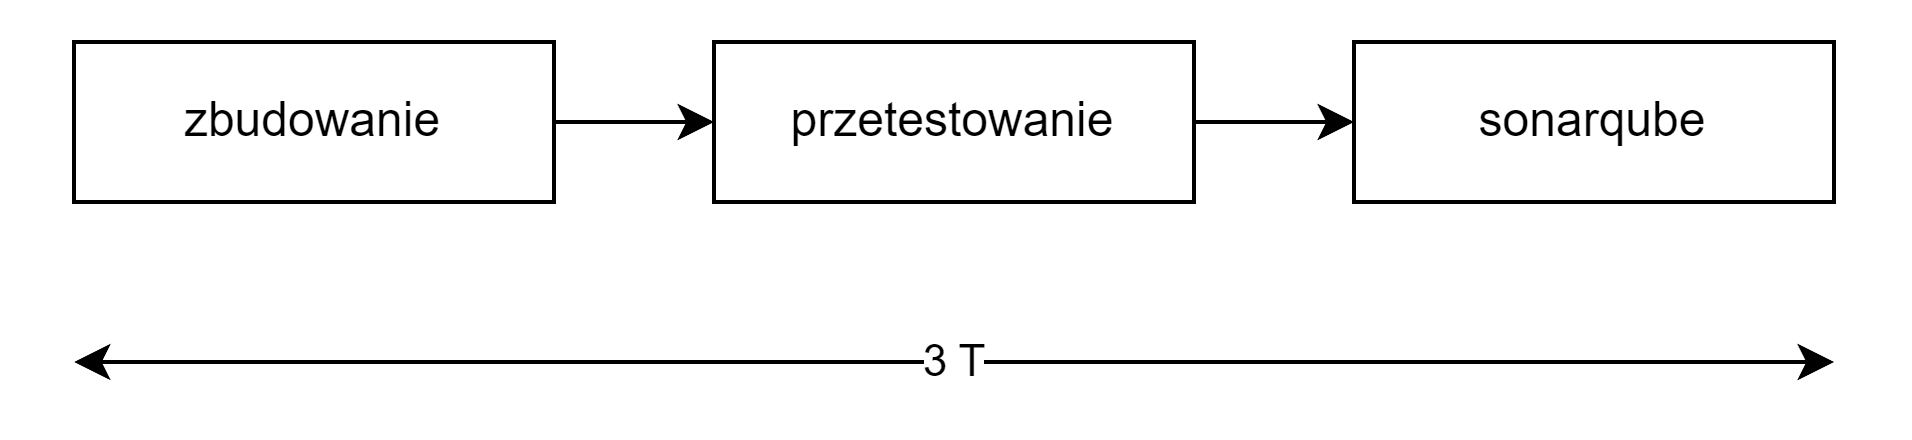
\includegraphics[width=1\linewidth]{pipelines3T.png}
    \caption{Czas trwania nieoptymalnego pipeline}
    \label{fig:enter-label}
\end{figure}

Warto jednak zauważyć, że krok \textbf{zbudowanie} musi być wykonany pierwszy, a kroki \textbf{przetestowanie} oraz \textbf{analiza kodu sonarqube} mogą być wykonane współbieżnie, ponieważ nie wpływają na siebie wzajemnie. Dobry rozdział na akcje pozwala w tym przypadku zaoszczędzić czas - cały pipeline wykona się teraz w 2 jednostki czasu.

\begin{figure}[H]
    \centering
    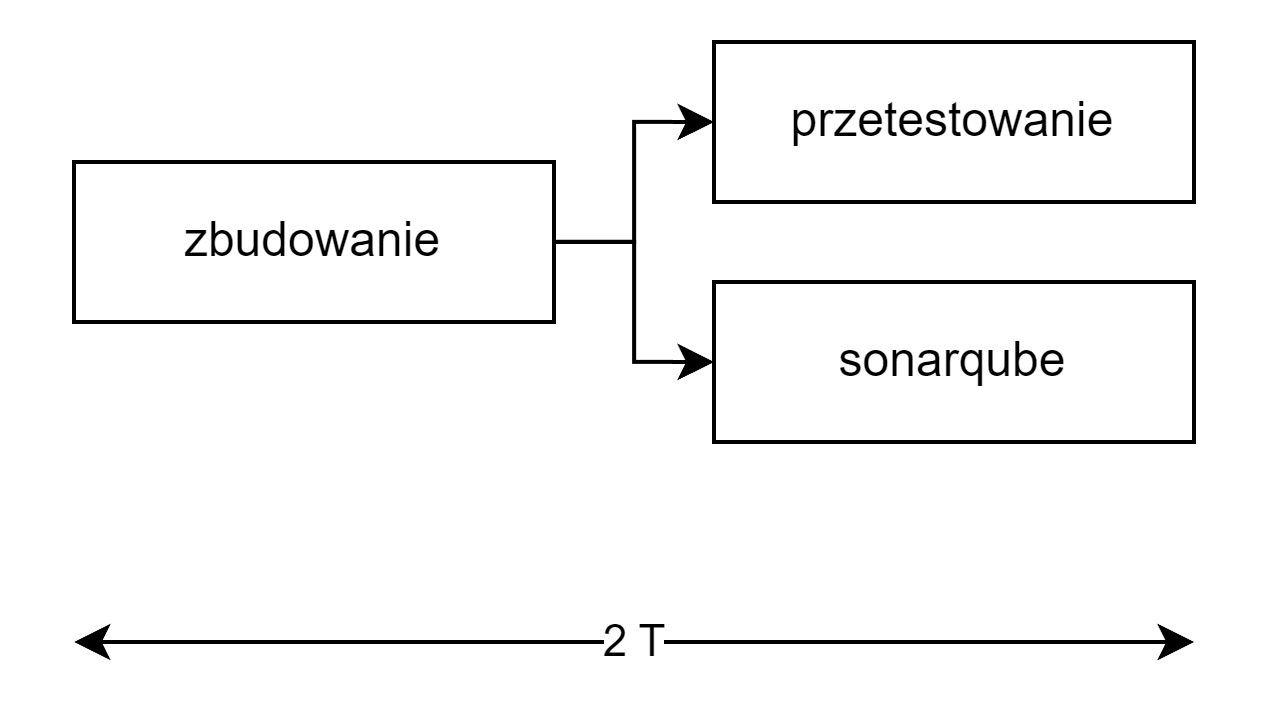
\includegraphics[width=0.5\linewidth]{pipelines2T.png}
    \caption{Czas trwania zoptymalizowanego pipeline}
    \label{fig:enter-label}
\end{figure}

\subsubsection{Abstrakcja}

Dobrze napisane akcje powinny być konfigurowalne i elastyczne, aby można było je wykorzystywać w różnych kontekstach, takich jak wdrażanie na środowiska deweloperskie i produkcyjne. Konfiguracja powinna odbywać się za pomocą parametrów, co pozwala na wielokrotne użycie tej samej akcji bez konieczności modyfikowania jej kodu.

\begin{figure}[H]
    \centering
    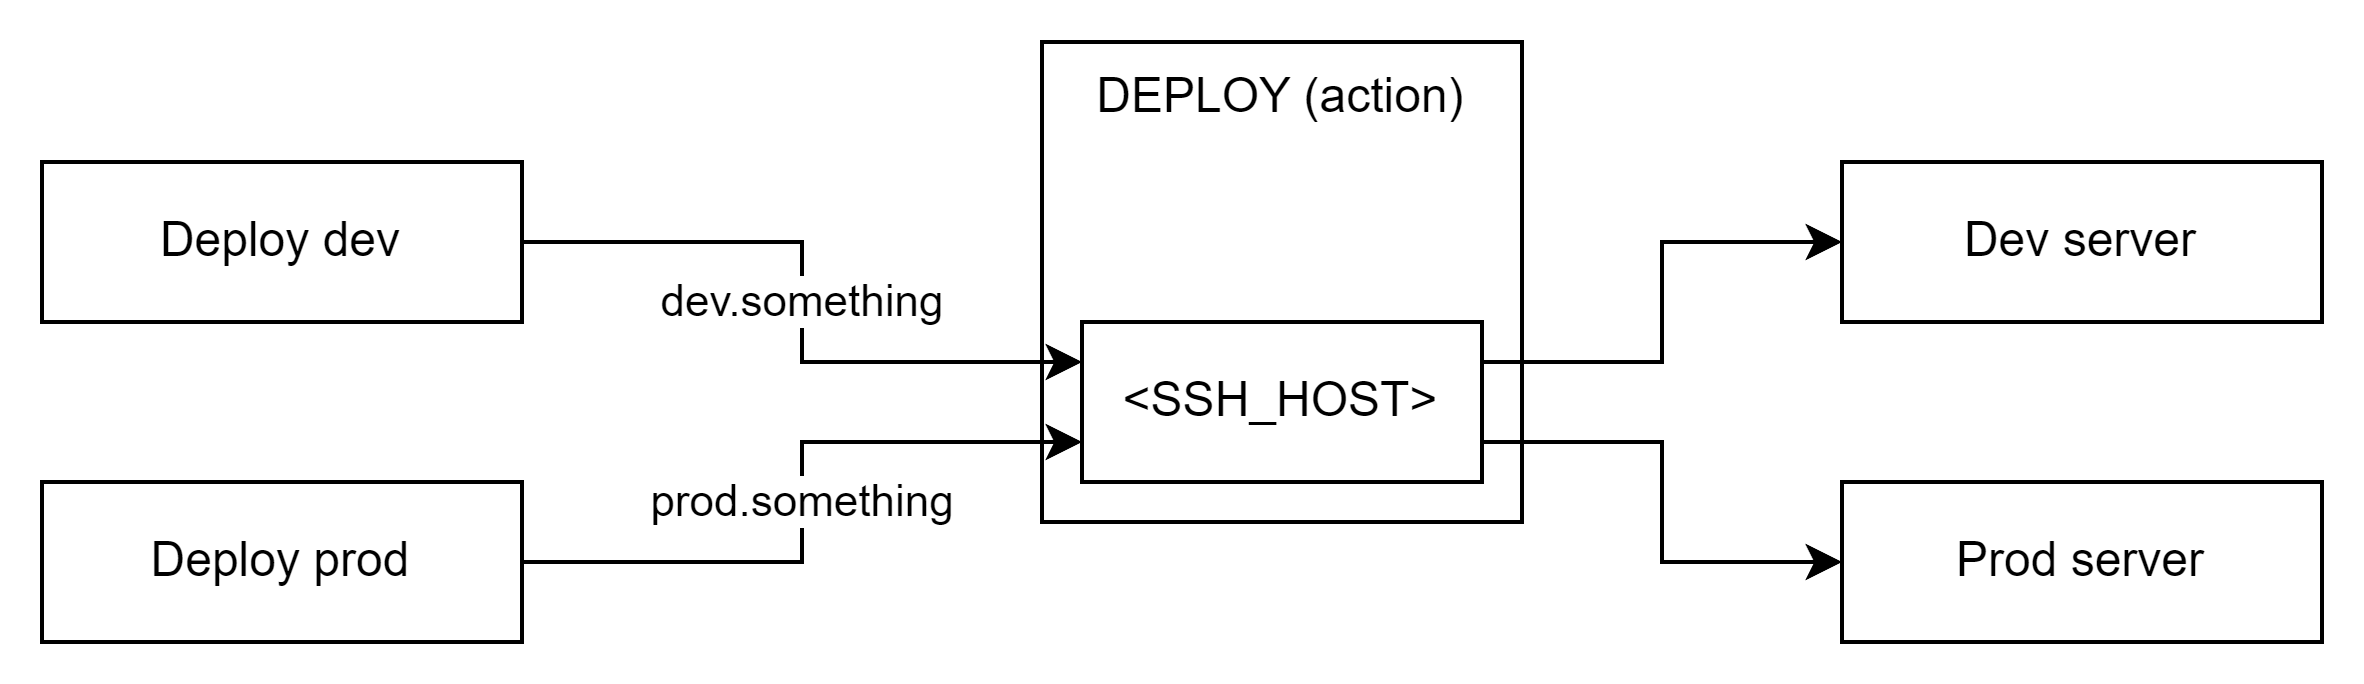
\includegraphics[width=1\linewidth]{pipelinesAbstraction.png}
    \caption{Abstrakcja w pipeline}
    \label{fig:enter-label}
\end{figure}

Możliwe jest także wyniesienie akcji na poziom wyższy niż obejmujący jedno repozytorium. Możliwe jest, że na przykład w skład projektu wchodzi kilka mikroserwisów napisanych w tej samej technologii. Wygodne jest wtedy stworzenie oddzielnego repozytorium na akcje i zdefiniowanie tam akcji powtarzalnych dla wszystkich tych mikroserwisów.

\subsubsection{Idempotencja}

Idempotencja jest kluczową zasadą w projektowaniu akcji CI/CD. Oznacza to, że wykonanie tej samej akcji wielokrotnie powinno dawać ten sam efekt, niezależnie od stanu początkowego. Idempotentne akcje minimalizują ryzyko wystąpienia błędów i nieprzewidzianych zachowań podczas wielokrotnego uruchamiania pipeline'u.

Przykładem nieidempotentnej akcji byłaby akcja budująca obraz dockerowy, która zaciąga repozytorium po prostu z brancha main. W tym wypadku o tym, co zostanie zbudowane decyduje aktualny stan brancha main. Po włączeniu pipeline, a następnie zmiany na branchu main i potem ponownym włączeniem tego samego pipeline zostanie zbudowany inny obraz.

Poprawnym rozwiązaniem tej sytuacji byłoby pobranie dokładnego commita, do którego referencji jest dostęp w samym pipeline. Ponowne włączenie tego samego pipeline zawsze będzie miało referencję do tego samego commita.

Przydatne może się to okazać w przypadku próby rollbacku do poprzedniej działającej wersji. Zakładając, że wdrożone zostały wersje:
\begin{itemize}
    \item wersja A - ta wersja zadziałała poprawnie,
    \item wersja B - ta wersja nie działa poprawnie
\end{itemize}

Można odszukać konkretny pipeline wdrażający wersję A i po prostu ponownie go włączyć. Zagwarantuje to ponowne wdrożenie działającej wersji.

\subsection{Więcej o języku opisu Github Actions}

W dalszej części pracy będę używał wiele takich samych wzorców. Wypiszę tutaj podstawowe wzorce używane w Github actions

\subsubsection{Triggery}

Zwykle chcemy, żeby pipeline włączał się po wykonaniu jakiejś akcji powiązanej z gitem. Język opisu Github actions udostępnia triggery, w środku których definiuje się, co ma spowodować rozpoczęcie danego pipeline. Najprostszym przykładem jest włączenia pipeline po zrobieniu akcji push na main.

\begin{lstlisting}[caption=Fragment kodu z triggerem ustawionym na push na main]
on:
  push:
    branches:
      - main
\end{lstlisting}


\subsubsection{Template}

Najprostszym sposobem napisania pipeline jest ten przytoczony wyżej. Stworzenie pliku \lstinline|.yml| i pisanie w nim kroków. Nie jest to jednak optymalny sposób, ponieważ uniemożliwia ponowne wykorzystanie powtarzalnych fragmentów kodu.

Powszechnie stosowaną praktyką jest podzielenie folderu z pipelinami na \lstinline|templates| oraz \lstinline|workflows|. Folder z templatami zawiera akcje konfigurowalne za pomocą parametrów. Folder z workflows natomiast po prostu je wywołuje.

\begin{figure}[H]
    \centering
    
\includegraphics[width=0.5\linewidth]{templatesAndWorkflows.png}
    \caption{Diagram przedstawiający w jaki sposób workflows korzystają z templates}
    \label{fig:enter-label}
\end{figure}

Aby przedstawić to na przykładzie, przygotowałem następujące pliki
\begin{lstlisting}[caption=Plik \lstinline|.github/templates/templateA/action.yml|]
name: Print message to the screen

inputs:
  message:
    required: true

runs:
  using: "composite"
  steps:
    - name: Print message to the screen
      shell: bash
      run: echo "${{ inputs.message }}"
\end{lstlisting}

\begin{lstlisting}[caption=Plik \lstinline|.github/workflows/workflowA.yml|]
name: Print message to the screen workflow (A)

on:
  push:
    branches:
      - main
jobs:
  main:
    runs-on: ubuntu-latest
    steps:
      - name: Checkout
        uses: actions/checkout@v3
      - name: Invoke print message to the screen
        uses: ./.github/templates/templateA
        with:
          message: "Hello world A!"
\end{lstlisting}

\begin{lstlisting}[caption=Plik \lstinline|.github/workflows/workflowB.yml|]
name: Print message to the screen workflow (B)

on:
  push:
    branches:
      - main
jobs:
  main:
    runs-on: ubuntu-latest
    steps:
      - name: Checkout
        uses: actions/checkout@v3
      - name: Invoke print message to the screen
        uses: ./.github/templates/templateA
        with:
          message: "Hello world B!"
\end{lstlisting}

Efektem wykonania akcji push na main jest włączenie dwóch pipelinów.

\begin{figure}[H]
    \centering
    
\includegraphics[width=1\linewidth]{testPipelinesInGithubActionsDashboard.png}
    \caption{Wycinek panelu Github actions}
    \label{fig:enter-label}
\end{figure}

I w każdym z nich odpowiedni tekst wypisany do konsoli 

\begin{figure}[H]
    \centering
    \begin{minipage}[b]{0.45\textwidth}
        \centering
        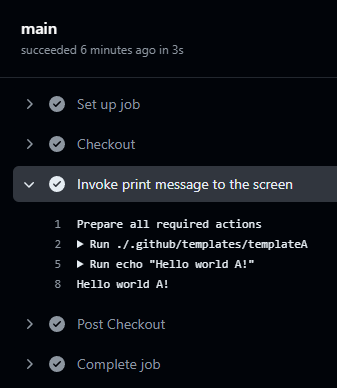
\includegraphics[width=\linewidth]{testPipelinesPipelineA.png}
        \caption{Efekt wykonania pipeline A}
        \label{fig:enter-label-a}
    \end{minipage}
    \hfill
    \begin{minipage}[b]{0.45\textwidth}
        \centering
        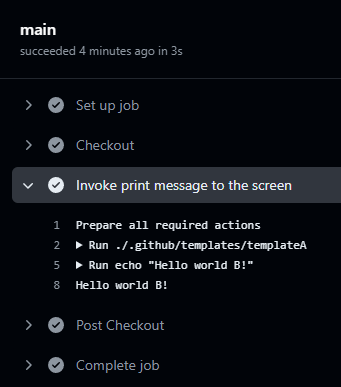
\includegraphics[width=\linewidth]{testPipelinesPipelineB.png}
        \caption{Efekt wykonania pipeline B}
        \label{fig:enter-label-b}
    \end{minipage}
\end{figure}

Przykładem stosowania templatów są multi środowiska. W dzisiejszym świecie kultura devops jest na tyle rozwinięta, że stosowanie kilku środowisk stało się standardem. Oznacza to, że oprócz produkcyjnego środowiska istnieje kopia (a czasem kilka) całkowicie wyizolowana od pozostałych środowisk. Zwykle dostępna pod adresem \lstinline|https://nazwa-środowiska.oryginalna-domena.pl|.

Rozwiązanie to jest wygodne, ponieważ pozwala przetestować zmiany w semi-realnym scenariuszu nie narażając środowiska produkcyjnego na błędy.

\section{Konfiguracja infrastruktury}

\subsection{Serwer}

Rolę mojego serwera będzie pełnić maszyna z ubuntu 22.04 posiadająca 2GB ramu, 10GB dysku oraz 1 współdzielony rdzeń procesora.

\subsection{Uwierzytelnienie do serwera}

W procesie uwierzytelniania do serwera VPS możemy wyróżnić dwa główne podejścia. Uwierzytelnienie kluczem SSH oraz uwierzytelnienie hasłem. Każde z tych rozwiązań ma swoje zalety i wady, które mogą wpływać na decyzję o wyborze jednej z metod w zależności od specyfiki użycia i wymagań bezpieczeństwa.

\subsubsection{Uwierzytelnienie hasłem}

Uwierzytelnienie hasłem jest jednym z najczęściej spotykanych i najprostszych sposobów zabezpieczania dostępu do serwera. Polega ono na wymaganiu od użytkownika podania nazwy użytkownika oraz odpowiadającego mu hasła podczas logowania.

\begin{itemize}
    \item \textbf{Zalety:}
    \begin{itemize}
        \item \textit{Łatwość użycia}: Proces logowania jest intuicyjny i nie wymaga zaawansowanej wiedzy technicznej.
        \item \textit{Powszechność}: Hasła są szeroko stosowane w różnych systemach i aplikacjach, co sprawia, że użytkownicy są zazwyczaj zaznajomieni z tą formą uwierzytelniania.
        \item \textit{Brak konieczności konfiguracji dodatkowego oprogramowania}: Nie wymaga instalacji czy konfiguracji dodatkowych narzędzi poza podstawową konfiguracją serwera.
    \end{itemize}
    \item \textbf{Wady:}
    \begin{itemize}
        \item \textit{Bezpieczeństwo}: Hasła mogą być narażone na ataki brute force, phishing, czy przechwytywanie podczas transmisji. Skuteczne hasło musi być odpowiednio długie i skomplikowane, co z kolei może być problematyczne do zapamiętania.
        \item \textit{Zarządzanie}: W przypadku wielu użytkowników lub często zmieniającego się personelu, zarządzanie hasłami może stać się trudne i czasochłonne.
        \item \textit{Skłonność do słabych haseł}: Użytkownicy często tworzą łatwe do odgadnięcia hasła, co zwiększa ryzyko nieautoryzowanego dostępu.
    \end{itemize}
\end{itemize}

\subsubsection{Uwierzytelnienie kluczem SSH}

Uwierzytelnienie kluczem SSH polega na użyciu pary kluczy kryptograficznych (klucza prywatnego i publicznego) do uwierzytelniania użytkownika. Klucz publiczny jest przechowywany na serwerze, natomiast klucz prywatny jest przechowywany przez użytkownika.

\begin{itemize}
    \item \textbf{Zalety:}
    \begin{itemize}
        \item \textit{Bezpieczeństwo}: Klucze SSH są znacznie trudniejsze do złamania w porównaniu z hasłami. Uwierzytelnianie kluczem prywatnym i publicznym zapewnia wysoki poziom bezpieczeństwa.
        \item \textit{Brak konieczności przesyłania klucza prywatnego}: Podczas procesu logowania klucz prywatny nigdy nie opuszcza maszyny użytkownika, co eliminuje ryzyko jego przechwycenia.
        \item \textit{Automatyzacja i skrypty}: Uwierzytelnienie kluczem jest wygodne do użycia w skryptach i automatycznych procesach, gdzie podanie hasła byłoby problematyczne.
    \end{itemize}
    \item \textbf{Wady:}
    \begin{itemize}
        \item \textit{Złożoność konfiguracji}: Proces generowania kluczy, ich instalacja i zarządzanie mogą być bardziej skomplikowane, zwłaszcza dla mniej doświadczonych użytkowników.
        \item \textit{Bezpieczeństwo klucza prywatnego}: Klucz prywatny musi być przechowywany w bezpiecznym miejscu. W przypadku jego utraty lub przechwycenia, dostęp do serwera może być zagrożony.
        \item \textit{Zarządzanie kluczami}: W dużych organizacjach zarządzanie kluczami może być skomplikowane, szczególnie jeśli użytkownicy często się zmieniają.
    \end{itemize}
\end{itemize}

\subsubsection{Implementacja}

Jako że uwierzytelnienie kluczem SSH jest bezpieczniejsze oraz wygodniejsze przy automatyzacji procesów, wybrałem właśnie tę opcję i opiszę proces implementacji.

Zwykle po wykupieniu serwera dostaje się dane do zalogowania. W tym hasło. Należy zalogować się do serwera tymi danymi. Następnie na swojej maszynie należy wygenerować parę kluczy ssh.

\begin{lstlisting}[caption=Wygenerowanie pary kluczy na swojej maszynie]
cd ~/.ssh
ssh-keygen -t rsa -b 4096
\end{lstlisting}

Stworzy to pliki \lstinline|id_rsa| oraz \lstinline|id_rsa.pub|. Należy skopiować zawartość \lstinline|id_rsa.pub|, a następnie wkleić ją do pliku \lstinline|~/.ssh/authorized_keys| na serwerze.

Ostatnim wygodnym krokiem jest stworzenie pliku \lstinline|~/.ssh/config| na lokalnej maszynie i dodanie tam konfiguracji serwera, gdzie \lstinline|IdentityFile| to ścieżka do prywatnego klucza SSH.

\begin{lstlisting}[caption=Przykładowa konfiguracja pliku config na lokalnej maszynie]
Host magisterka
    HostName srv15.mikr.us
    User root
    Port 10104
    IdentityFile ~/.ssh/id_rsa
    IdentitiesOnly yes
    ServerAliveInterval 60
\end{lstlisting}

Po wykonaniu powyższych kroków można przetestować połączenie z serwerem wpisując w terminal \lstinline|ssh magisterka|. Powinno to połączyć się z serwerem.

Parametr \lstinline|ServerAliveInterval| zadba o to, żeby sesja z serwerem nie zamykała się od nieaktywności. Maszyna hosta co 60 sekund będzie wysyłała do serwera ping, co spowoduje utrzymanie otwartego połączenia.


\subsection{Instalacja potrzebnych narzędzi}

Jak wspomniane wcześniej, należy zminimalizować liczbę potrzebnych zależności na serwerze. W tym wypadku potrzebny będzie jedynie Docker, którego można zainstalować wykonując:

\begin{lstlisting}[caption=Skrypt instalujący dockera na maszynie Ubuntu]
curl -fsSL https://get.docker.com -o get-docker.sh
sh get-docker.sh
\end{lstlisting}

Należy przeprowadzić weryfikację poprawnej instalacji używając \lstinline|docker ps|. Powinna pokazać się Dockerowa tabelka pokazująca, że aktualnie nie pracują żadne kontenery:

\begin{lstlisting}[caption=Wynik wykonania komendy weryfikującej instalację Dockera]
root@l104:~# docker ps
CONTAINER ID   IMAGE     COMMAND   CREATED   STATUS    PORTS     NAMES
\end{lstlisting}


\subsection{Tunelowanie IPv6}

Jako że serwer wybrany przeze mnie należy do budżetowych, nie ma on swojego adresu IPv4. Jest to popularna praktyka obniżająca koszty. Dostawca zapewnia wtedy adres IPv6, do którego jednak nie wszyscy użytkownicy mają dostęp (adres IPv6 nie jest powszechnie wspierany).

Aby to obejść, można skorzystać z darmowego narzędzia \textbf{Cloudflare}, do którego najpierw należy podpiąć swoją domenę. Cloudflare będzie pełniło rolę proxy. Użytkownik wchodząc na domenę będzie łączył się z Cloudflare po IPv4, a ten będzie tunelował ten ruch trybem IPv6 do serwera.

\begin{figure}[H]
    \centering
    
\includegraphics[width=1\linewidth]{ipv6diagram.png}
    \caption{Zasada działania tunelowania IPv6 Cloudflare}
    \label{fig:enter-label}
\end{figure}

W pierwszej kolejności należy na serwerze wykonać komendę \lstinline|ifconifg|, aby dostać się do listy interfejsów sieciowych serwera. Następnie odszukać pole \lstinline|inet6| i skopiować jego wartość.

\begin{figure}[H]
    \centering
    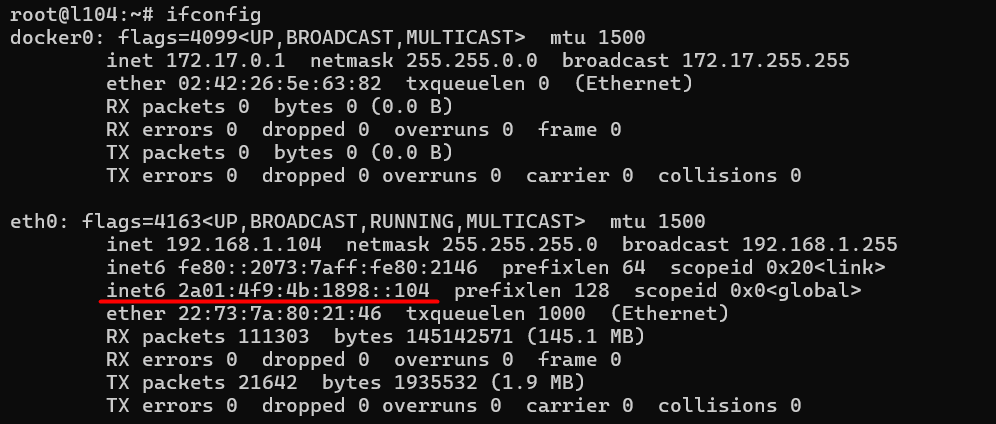
\includegraphics[width=1\linewidth]{ipv6server.png}
    \caption{Lista interfejsów sieciowych serwera z adresem IPv6 serwera zaznaczonym na czerwono}
    \label{fig:enter-label}
\end{figure}

Następnie w sekcji \textbf{DNS} panelu konfiguracyjnego domeny w Cloudflare należy dodać rekord AAAA z nazwą ustawioną na nazwę domeny, a wartością ustawioną na wcześniej skopiowany adres.

\begin{figure}[H]
    \centering
    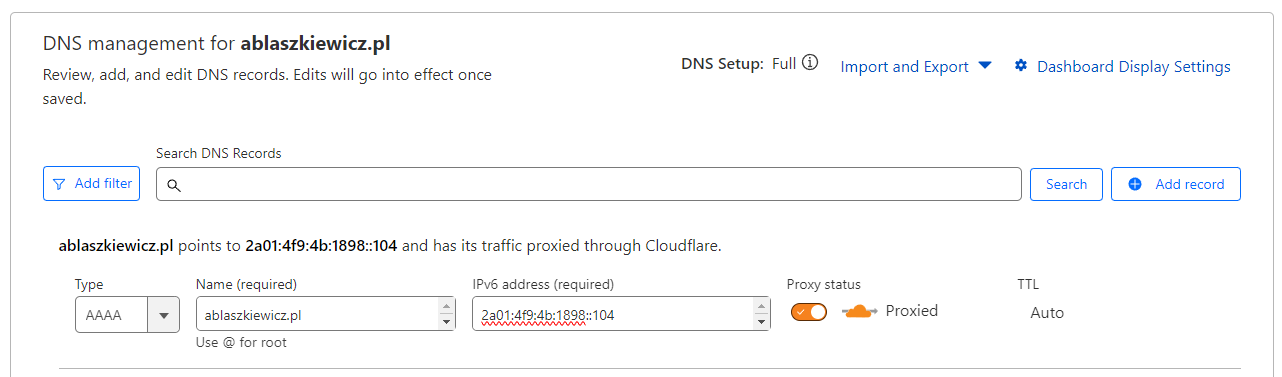
\includegraphics[width=1\linewidth]{ipv6cloudflare.png}
    \caption{Dodanie rekordu AAAA w Cloudflare}
    \label{fig:enter-label}
\end{figure}

Aby upewnić się, że konfiguracja działa, należy na serwerze postawić testowy kontener z obrazem \textbf{nginx} używając \lstinline|docker run -p 80:80 nginx|


W celu weryfikacji poprawności wszystkich kroków należy udać się na stronę domeny (w tym wypadku ablaszkiewicz.pl). Strona powinna pokazać stronę startową \textbf{nginx}.

\begin{figure}[H]
    \centering
    
\includegraphics[width=1\linewidth]{ipv6helloWorld.png}
    \caption{Strona startowa nginx}
    \label{fig:enter-label}
\end{figure}


\section{Reverse proxy}

\subsection{Idea}

W aktualnej konfiguracji z poziomu domeny można dostać się tylko do jednego serwisu działającego na serwerze - konkretnie do serwisu działającego na porcie 80. Jest to oczywiście niechciane rozwiązanie, ponieważ w aktualnej konfiguracji na serwerze włączone będą minimum 2 serwisy - frontend oraz backend.

Aby radzić sobie z takimi sytuacjami, wykorzystuje się mechanizm zwany \textbf{reverse proxy}. Zamiast uruchamiać serwis bezpośrednio na porcie 80, to na porcie 80 stawia się reverse proxy, któremu podaje się zestaw reguł, na podstawie których kieruje ono ruch na inne, wewnętrzne porty serwera.

W klasycznym podejściu do reverse proxy instaluje się narzędzie typu nginx w warstwie systemowej i to tutaj się je konfiguruje. Znacząco lepszym pomysłem i łatwiejszym pomysłem jest jednak zdockeryzowanie reverse proxy. Ingerencja w usługi systemowe zawsze wiąże się z ryzykiem - możliwe, że konfiguracja będzie błędna i bardzo dużo czasu zajmie odnalezienie błędu - zdockeryzowanie narzędzia pozwoli uodpornić się na błędy konfiguracji oraz zapewni powrót do poprzednich, działających wersji w przypadku błędów.

\subsection{Implementacja}

Narzędziem realizującym to zadanie w moim przypadku będzie nginx. Oprócz wyżej wymienionego zadania warto wiedzieć, że narzędzia tego typu zwykle zbierają logi wszystkiego, co związane z przekierowaniami. Będzie to bardzo przydatne w dalszej części pracy.

Narzędzie skonfigurowałem tak, aby domyślnie kierowało ruch na wewnętrzny port serwera 3000 (tam będzie działał frontend), a adresy zawierające \lstinline|/api/| kierowało na 3001 (tam będzie działał backend).

\begin{figure}[H]
    \centering
    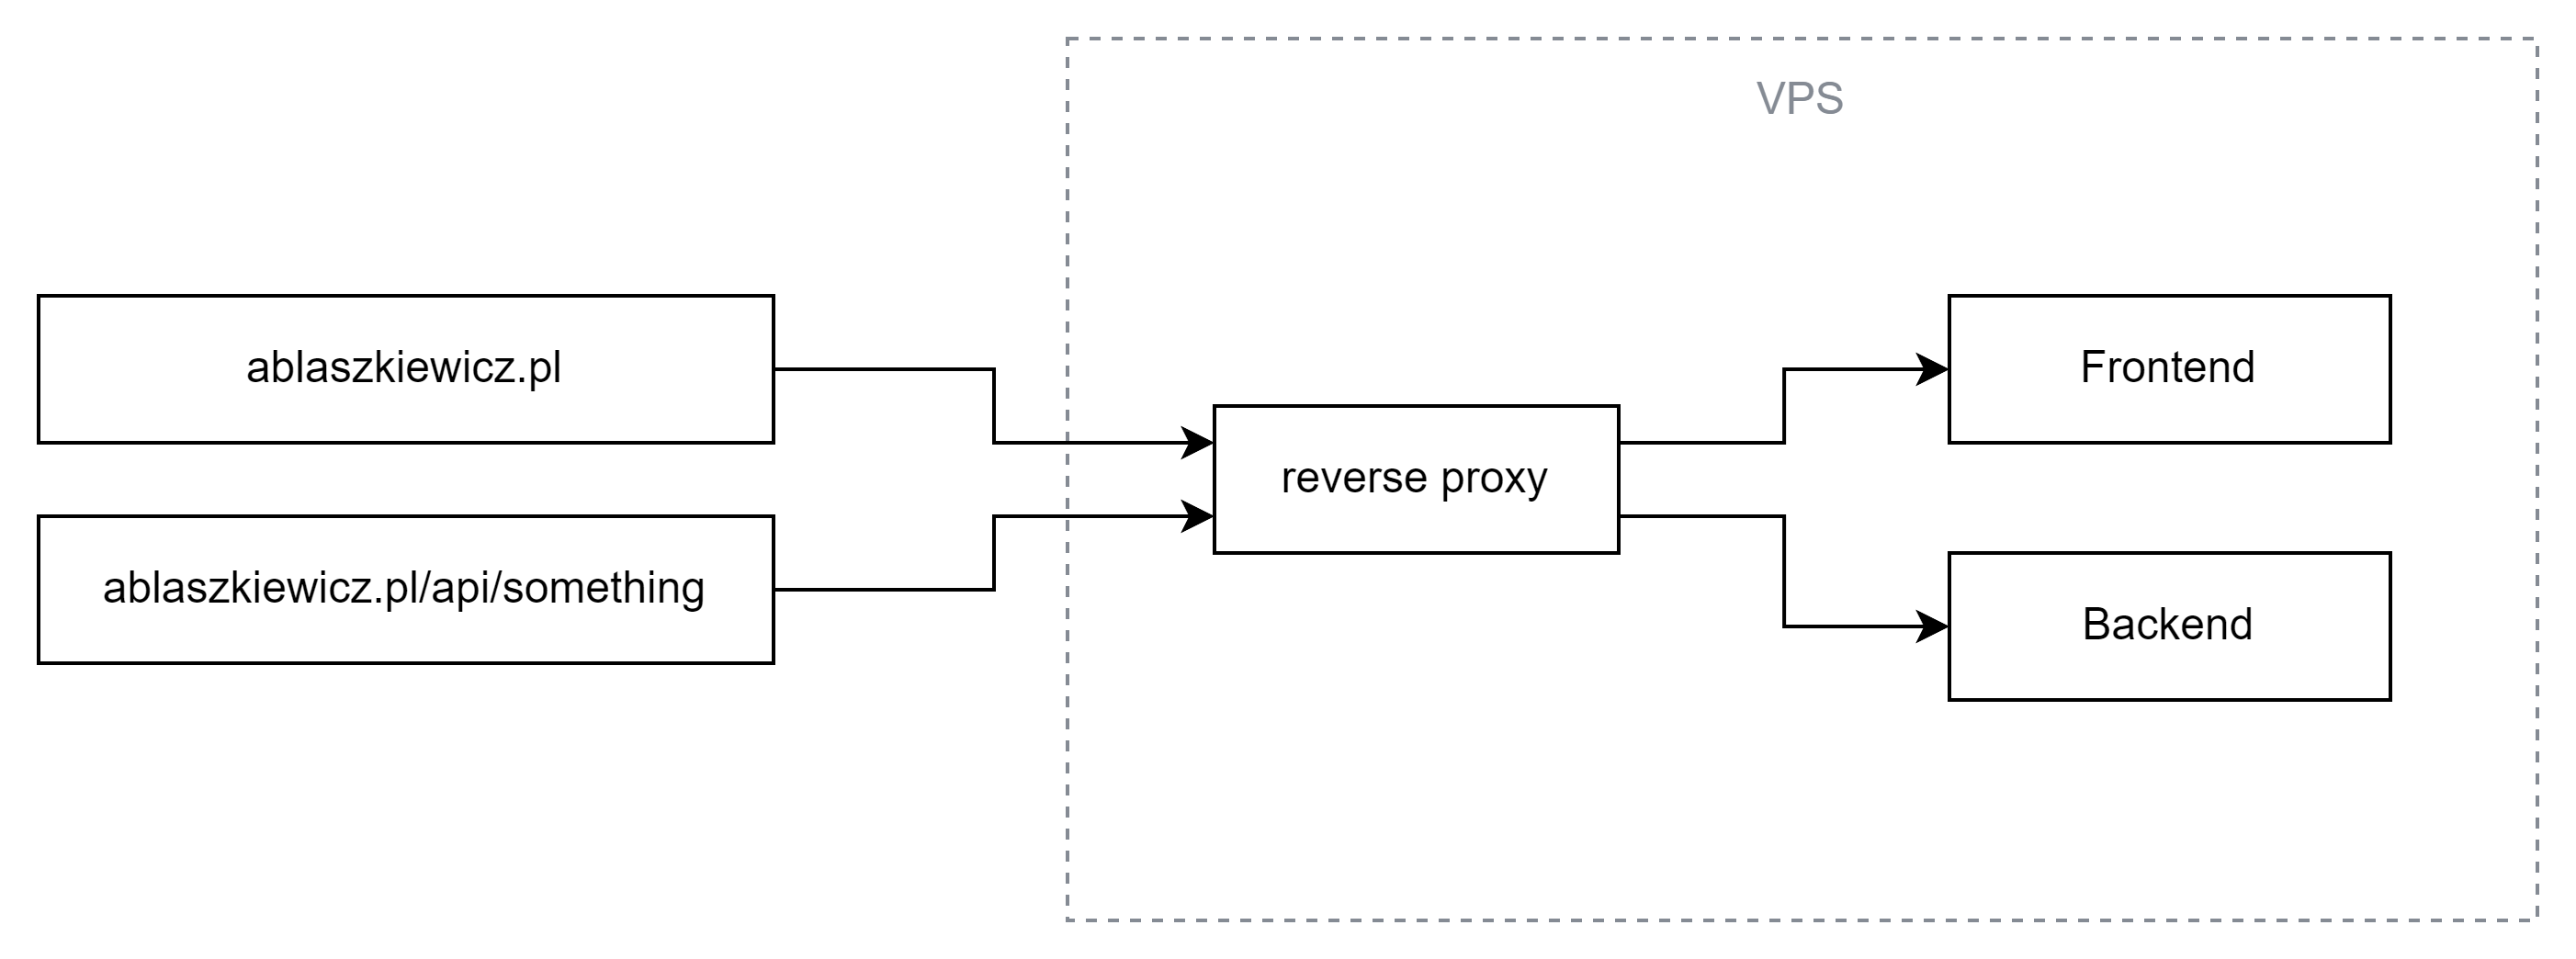
\includegraphics[width=1\linewidth]{reverseProxyDiagram.png}
    \caption{Zasada działania reverse proxy}
    \label{fig:enter-label}
\end{figure}

W tym celu przygotowałem pliki, które zbudują obraz dockerowy z reverse proxy.

\begin{lstlisting}[caption=Plik \lstinline|/infrastructure/reverse-proxy/Dockerfile|]
FROM nginx:1.22.0-alpine

WORKDIR /

COPY ./src/nxconf.sh /

RUN chmod +x /nxconf.sh && /nxconf.sh

RUN mkdir -p /var/log/nginx /var/cache/nginx /var/run/nginx && \
    chown -R nginx:nginx /var/log/nginx /var/run/nginx /var/cache/nginx /etc/nginx && \
    sed -e 's#/var/run/nginx.pid#/var/run/nginx/nginx.pid#' -e '/user  nginx;/d'  -i /etc/nginx/nginx.conf

RUN echo "server_names_hash_bucket_size 128;" >/etc/nginx/conf.d/_server_name_hash.conf

RUN echo "client_max_body_size 1g;" >/etc/nginx/conf.d/my_proxy.conf
RUN echo -e "map \$http_upgrade \$connection_upgrade {\n default upgrade;\n '' close;\n}" >/etc/nginx/conf.d/_websocks.conf

EXPOSE 3080

USER nginx

CMD ["nginx", "-g", "daemon off;"]
\end{lstlisting}

\begin{lstlisting}[caption=Plik \lstinline|/infrastructure/reverse-proxy/src/nxconf.sh|]
#!/bin/sh
out="/etc/nginx/conf.d/default.conf"
domain="ablaszkiewicz.pl"
frontend_path="http://192.168.1.104:3000"
backend_path="http://192.168.1.104:3001/"

echo -n > "$out"

config=$(cat <<EOF
server {
    listen       80;
    listen  [::]:80;
    server_name  $domain;

    location = / {
        proxy_pass $frontend_path;
        proxy_set_header Host \$host;
        proxy_http_version 1.1;
        proxy_set_header Upgrade \$http_upgrade;
        proxy_set_header Connection \$connection_upgrade;
        proxy_ssl_name \$host;
        proxy_ssl_server_name on;
        proxy_ssl_verify off;
        proxy_ssl_protocols  TLSv1 TLSv1.1 TLSv1.2;
        proxy_ssl_session_reuse off;
        proxy_set_header X-Forwarded-For \$remote_addr;
        proxy_set_header X-Forwarded-Proto \$scheme;
        proxy_read_timeout 120;
        proxy_send_timeout 120;
        proxy_connect_timeout 120;
    }

    location /api/ {
        proxy_pass $backend_path;
        proxy_set_header Host \$host;
        proxy_http_version 1.1;
        proxy_set_header Upgrade \$http_upgrade;
        proxy_set_header Connection \$connection_upgrade;
        proxy_ssl_name \$host;
        proxy_ssl_server_name on;
        proxy_ssl_verify off;
        proxy_ssl_protocols  TLSv1 TLSv1.1 TLSv1.2;
        proxy_ssl_session_reuse off;
        proxy_set_header X-Forwarded-For \$remote_addr;
        proxy_set_header X-Forwarded-Proto \$scheme;
        proxy_read_timeout 120;
        proxy_send_timeout 120;
        proxy_connect_timeout 120;
    }
}
EOF
)

echo "$config" >> "$out"
\end{lstlisting}

\subsection{Test}

W celu przetestowania podejścia wykonałem na serwerze serię komend

\begin{lstlisting}[caption=Komendy włączające reverse proxy na serwerze]
git clone https://github.com/ablaszkiewicz/devops-sandbox.git
cd devops-sandbox/infrastructure/reverse-proxy
docker build -t reverse-proxy .
docker run -p 80:80 -d reverse-proxy
docker run -p 3000:80 -d nginx
docker run -p 3001:80 -d httpd
\end{lstlisting}

Powyższe komendy uruchamiają serwisy w następującej konfiguracji:
\begin{itemize}
    \item port 80 - napisane reverse proxy,
    \item port 3000 - bazowy obraz nginx,
    \item port 3001 - bazowy obraz apache
\end{itemize}

Po włączeniu wszystkich kontenerów po wejściu na \lstinline|https://ablaszkiewicz.pl| powinna ukazać się strona startowa nginx

\begin{figure}[H]
    \centering
    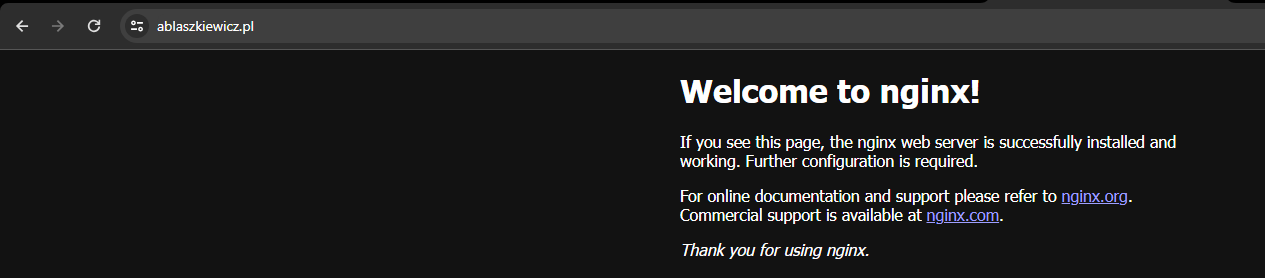
\includegraphics[width=1\linewidth]{reverseProxyNginx.png}
    \caption{Strona startowa nginx}
    \label{fig:enter-label}
\end{figure}

A po wejściu na \lstinline|https://ablaszkiewicz.pl/api| powinna ukazać się strona startowa apache

\begin{figure}[H]
    \centering
    
\includegraphics[width=1\linewidth]{reverseProxyApache.png}
    \caption{Strona startowa Apache}
    \label{fig:enter-label}
\end{figure}

\subsection{Wiele środowisk}

W idealnym świecie każde środowisko powinno być oddzielną maszynę. Z uwagi na budżet u mnie jednak obydwa środowiska będą działały na jednej maszynie i wytłumaczę podejście, które zastosowałem do osiągnięcia dobrze zarządzalnego kierowania ruchem. Poprzednio zaimplementowane reverse proxy działa na poziomie lokalizacji (dobiera to, co znajduje się już po \lstinline|.pl|), dlatego nazwę je \lstinline|location reverse proxy|. Nowe reverse proxy będzie dobierało to, co znajduje się przed nazwą domeny, dlatego nazwę je \lstinline|domain reverse proxy|.

W mojej konfiguracji będzie istniało środowisko produkcyjne dostępne pod standardową domeną oraz środowisko deweloperskie dostępne z prefixem \lstinline|dev.|.

Nowo powstałe reverse proxy zostanie wpięte przed reverse proxy odpowiedzialnymi za lokalizację, tworząc następującą strukturę

\begin{figure}[H]
    \centering
    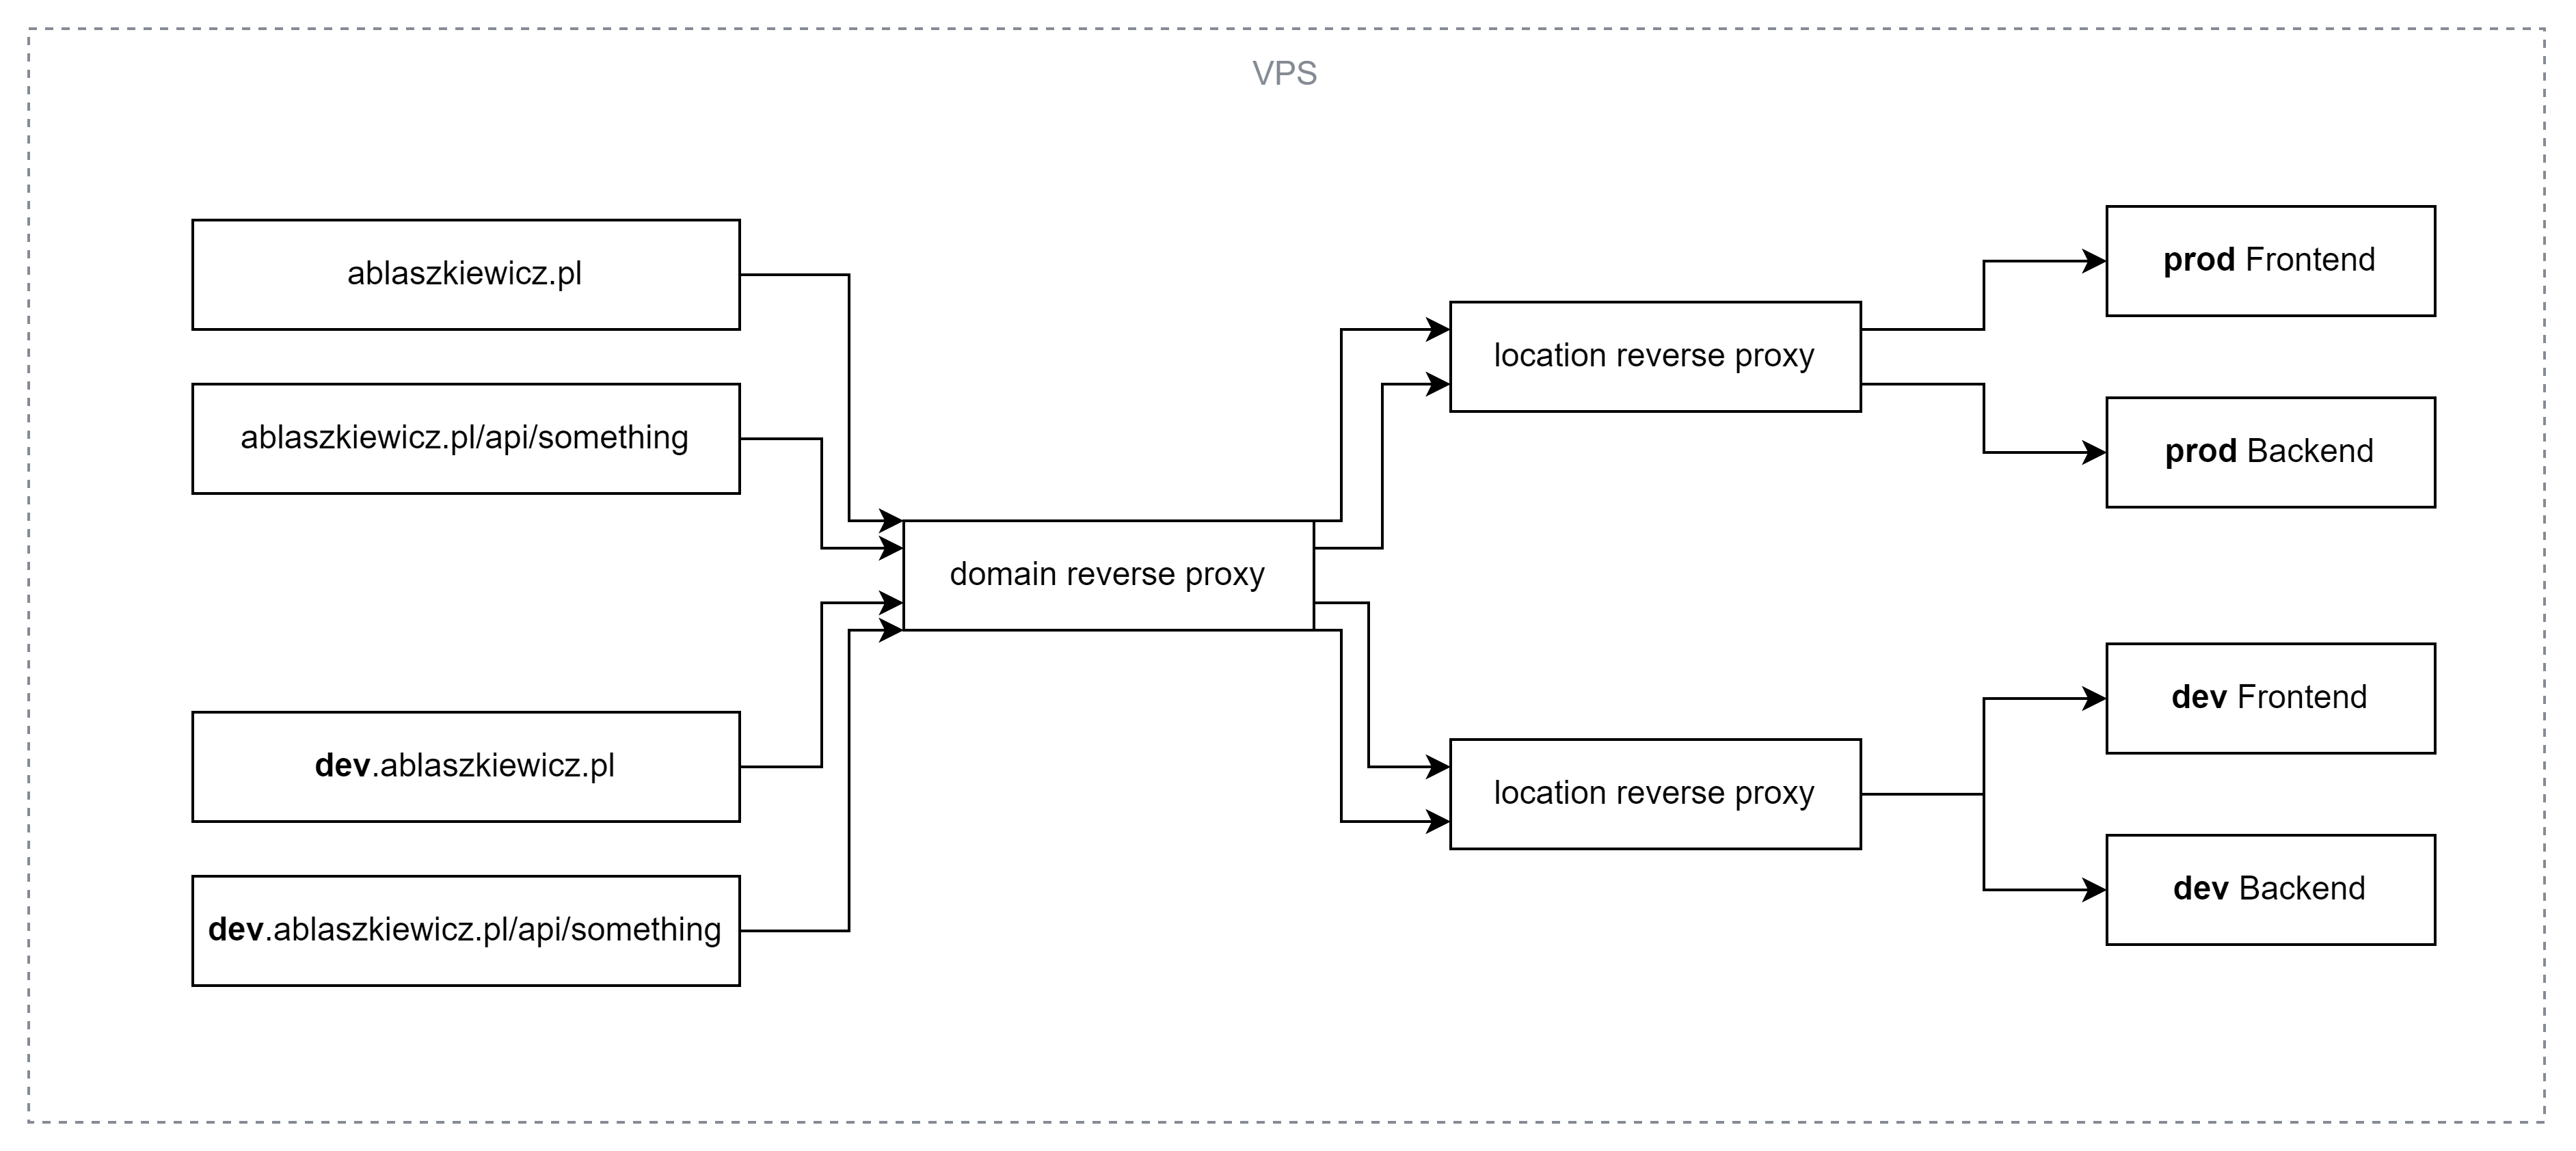
\includegraphics[width=1\linewidth]{domainReverseProxy.png}
    \caption{Diagram przedstawiający zasadę działania reverse proxy przy wielu środowiskach na jednej maszynie}
    \label{fig:enter-label}
\end{figure}


Zasada konfiguracji reverse proxy jest analogiczna do poprzednich. Jako że zasady przekierowań są tutaj bardzo proste, skorzystam z wrappera \lstinline|https://github.com/unkn0w/proxer|, który udostępnia prosty plik konfiguracyjny definiujący zasady przekierowań i też jest zdockeryzowany.

\begin{lstlisting}[caption=Plik \lstinline|/infrastructure/reverse-proxy/src/nxconf.sh|]
my.domain1.com=http://192.168.1.123:3000
my.domain2.com=http://192.168.1.222:8080
my.otherdomain.org=http://somedomain.com
\end{lstlisting}

\subsection{Pipeline}

\subsubsection{Definicja pipeline'u}

Pipeline dla backendu będzie składał się z następujących kroków:

\begin{itemize}
    \item zbudowanie obrazu Docker,
    \item wypchnięcie obrazu Docker do rejestru,
    \item wdrożenie aplikacji na serwer.
\end{itemize}

\begin{figure}[H]
    \centering
    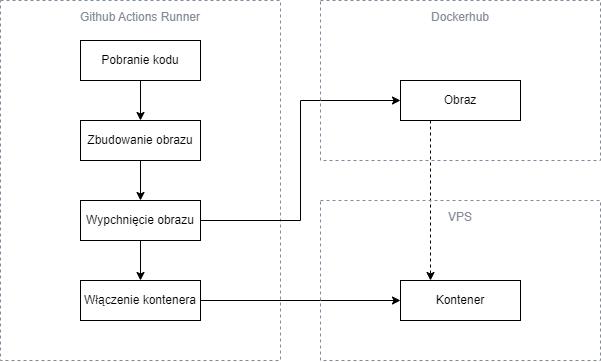
\includegraphics[width=0.75\linewidth]{githubActionsSchema.png}
    \caption{Diagram przedstawiający zasadę działania pipeline do wdrożenia}
    \label{fig:enter-label}
\end{figure}

\subsubsection{Template}

Jako że akcja zbudowania i wypchnięcia obrazu do rejestru jest wspólna nie tylko dla reverse proxy, stworzyłem dedykowany, generyczny template \lstinline|.github/templates/build-and-push/action.yml|, który jako parametry wejściowe przyjmuje dane uwierzytelniające do Dockerhub, kontekst, ścieżkę do pliku \lstinline|Dockerfile| oraz nazwę obrazku. Akcja buduje obraz, a następnie wypycha go do rejestru zgodnie z podanymi danymi.


Akcja wdrożenia reverse proxy również jest wspólna nie tylko dla reverse proxy, dlatego stworzyłem template \lstinline|.github/templates/deploy-container/action.yml|, który jako parametry wejściowe przyjmuje dane uwierzytelniające do serwera, nazwę obrazu, nazwę kontenera oraz parę portów. Akcja loguje się do serwera i włącza kontener zgodnie z podanymi danymi

\begin{figure}[H]
    \centering
    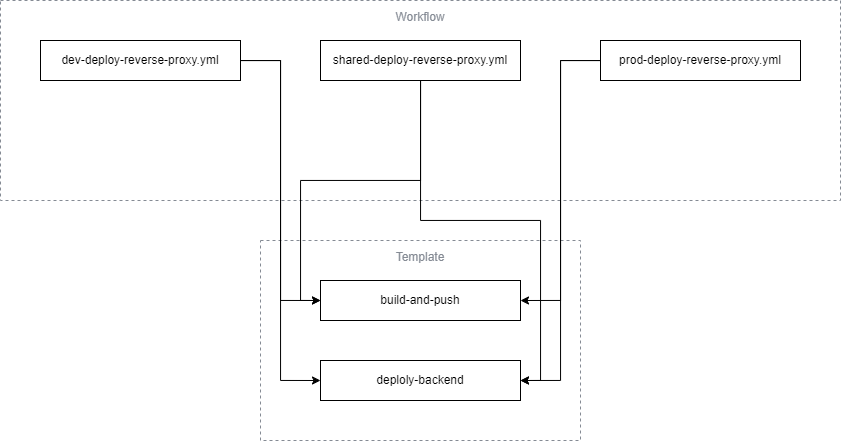
\includegraphics[width=1\linewidth]{reverseProxyTemplatesSchema.png}
    \caption{Diagram przedstawiający użycie template i workflow przy wdrażaniu reverse proxy}
    \label{fig:enter-label}
\end{figure}

\begin{lstlisting}[caption=Plik \texttt{.github/templates/build-and-push/action.yml}]
name: Build and push

inputs:
  # Context
  context:
    required: true
  file:
    required: true

  # Dockerhub
  dockerhub-username:
    required: true
  dockerhub-token:
    required: true
  image-name:
    required: true

runs:
  using: 'composite'
  steps:
    - name: Checkout
      uses: actions/checkout@v3
    - name: Set up QEMU
      uses: docker/setup-qemu-action@v1
    - name: Set up Docker Buildx
      uses: docker/setup-buildx-action@v1
    - name: Login to DockerHub
      uses: docker/login-action@v1
      with:
        username: ${{ inputs.dockerhub-username }}
        password: ${{ inputs.dockerhub-token }}
    - name: Build and push
      id: docker_build
      uses: docker/build-push-action@v2
      with:
        context: ${{ inputs.context }}
        file: ${{ inputs.file }}
        push: true
        tags: ${{ inputs.image-name }}:latest
\end{lstlisting}

\begin{lstlisting}[caption=Plik \texttt{.github/templates/deploy-container/action.yml}]
name: Deploy

inputs:
  # SSH
  host:
    required: true
  username:
    required: true
  port:
    required: true
  ssh-private-key:
    required: true

  # Docker
  image-name:
    required: true
  server-port:
    required: true
  container-name:
    required: true
  application-port:
    required: true

runs:
  using: 'composite'
  steps:
    - name: Update image inside VPS
      uses: appleboy/ssh-action@master
      with:
        host: ${{ inputs.host }}
        USERNAME: ${{ inputs.username }}
        PORT: ${{ inputs.port }}
        KEY: ${{ inputs.ssh-private-key }}
        script: |
          docker rm -f ${{ inputs.container-name }}
          docker pull ${{ inputs.image-name }}
          docker run -d \
          -p ${{ inputs.server-port }}:${{ inputs.application-port }} \
          --restart=always \
          --name ${{ inputs.container-name }} \
          ${{ inputs.image-name }}
\end{lstlisting}

\subsubsection{Workflow}

Poprzednio zdefiniowane template wystarczy teraz tylko wywołać. W sumie będą to 3 pliki workflow tworzące wcześniej wspomniane

\begin{itemize}
    \item domain reverse proxy - odpowiedzialne za dzielenie ruchu pomiędzy środowiskami,
    \item 2 location reverse proxy - odpowiedzialne za dzielenie ruchu pomiędzy frontend a backend na konkretnym środowisku.
\end{itemize}

Warto zauważyć, że pliki mają bardzo mało różnic. Głównie będzie to nazwa obrazu i port, na którym włączony zostanie kontener. Przyjmuję, że kontenery produkcyjne będą działały na portach \lstinline|30XX|, a deweloperskie na \lstinline|40XX|. 

\begin{lstlisting}[caption=Plik \texttt{.github/workflows/dev-deploy-reverse-proxy.yml}]
name: Deploy reverse proxy (dev)

on:
  workflow_dispatch:
  push:
    branches:
      - 'main'

jobs:
  deploy:
    runs-on: ubuntu-latest
    steps:
      - name: Checkout
        uses: actions/checkout@v3
      - name: Build and push
        uses: './.github/templates/build-and-push'
        with:
          context: ./infrastructure/reverse-proxy-dev
          file: ./infrastructure/reverse-proxy-dev/Dockerfile
          dockerhub-username: ${{ secrets.DOCKERHUB_USERNAME }}
          dockerhub-token: ${{ secrets.DOCKERHUB_TOKEN }}
          image-name: ablaszkiewicz/magisterka-reverse-proxy-dev
      - name: Deploy
        uses: './.github/templates/deploy-container'
        with:
          host: ${{ secrets.SSH_HOST }}
          username: ${{ secrets.SSH_USER }}
          port: ${{ secrets.SSH_PORT }}
          ssh-private-key: ${{ secrets.SSH_KEY }}
          server-port: 4080
          application-port: 80
          image-name: ablaszkiewicz/magisterka-reverse-proxy-dev
          container-name: magisterka-reverse-proxy-dev

\end{lstlisting}

\begin{lstlisting}[caption=Plik \texttt{.github/workflows/prod-deploy-reverse-proxy.yml}]
name: Deploy reverse proxy (prod)

on:
  workflow_dispatch:
  push:
    branches:
      - 'main'

jobs:
  deploy:
    runs-on: ubuntu-latest
    steps:
      - name: Checkout
        uses: actions/checkout@v3
      - name: Build and push
        uses: './.github/templates/build-and-push'
        with:
          context: ./infrastructure/reverse-proxy-prod
          file: ./infrastructure/reverse-proxy-prod/Dockerfile
          dockerhub-username: ${{ secrets.DOCKERHUB_USERNAME }}
          dockerhub-token: ${{ secrets.DOCKERHUB_TOKEN }}
          image-name: ablaszkiewicz/magisterka-reverse-proxy-prod
      - name: Deploy
        uses: './.github/templates/deploy-container'
        with:
          host: ${{ secrets.SSH_HOST }}
          username: ${{ secrets.SSH_USER }}
          port: ${{ secrets.SSH_PORT }}
          ssh-private-key: ${{ secrets.SSH_KEY }}
          server-port: 3080
          application-port: 80
          image-name: ablaszkiewicz/magisterka-reverse-proxy-prod
          container-name: magisterka-reverse-proxy-prod

\end{lstlisting}

\begin{lstlisting}[caption=Plik \texttt{.github/workflows/shared-deploy-reverse-proxy.yml}]
name: Deploy reverse proxy (shared)

on:
  workflow_dispatch:
  push:
    branches:
      - 'main'

jobs:
  deploy:
    runs-on: ubuntu-latest
    steps:
      - name: Checkout
        uses: actions/checkout@v3
      - name: Build and push
        uses: './.github/templates/build-and-push'
        with:
          context: ./infrastructure/reverse-proxy-shared
          file: ./infrastructure/reverse-proxy-shared/Dockerfile
          dockerhub-username: ${{ secrets.DOCKERHUB_USERNAME }}
          dockerhub-token: ${{ secrets.DOCKERHUB_TOKEN }}
          image-name: ablaszkiewicz/magisterka-reverse-proxy-shared
      - name: Deploy
        uses: './.github/templates/deploy-container'
        with:
          host: ${{ secrets.SSH_HOST }}
          username: ${{ secrets.SSH_USER }}
          port: ${{ secrets.SSH_PORT }}
          ssh-private-key: ${{ secrets.SSH_KEY }}
          server-port: 80
          application-port: 80
          image-name: ablaszkiewicz/magisterka-reverse-proxy-shared
          container-name: magisterka-reverse-proxy-shared

\end{lstlisting}

\subsection{Zestawienie}

Przygotowałem poniżej zestawienie, które prezentuje wyższość rozwiązania wykorzystującego zdockeryzowane reverse proxy ponad standardowym.

\begin{table}[H]
\centering
\begin{tabular}{|l|c|c|c|}
\hline
\textbf{Cecha} & \textbf{Brak reverse proxy} & \textbf{Reverse proxy} & \textbf{+docker} \\ \hline
Kilka serwisów na tym samym porcie & \cellcolor{red!50}nie & \cellcolor{green!50}tak & \cellcolor{green!50}tak \\ \hline
Bogate logi  & \cellcolor{yellow!50}po stronie aplikacji & \cellcolor{green!50}tak & \cellcolor{green!50}tak \\ \hline
Ukrycie wewnętrznych zasad routingu & \cellcolor{red!50}nie & \cellcolor{green!50}tak & \cellcolor{green!50}tak \\ \hline
Banowanie lokalizacji & \cellcolor{yellow!50}po stronie aplikacji & \cellcolor{green!50}tak & \cellcolor{green!50}tak \\ \hline
Centralne zarządzanie ruchem & \cellcolor{red!50}nie & \cellcolor{green!50}tak & \cellcolor{green!50}tak \\ \hline
Odporność na błędy konfiguracji & \cellcolor{yellow!50}nie dotyczy & \cellcolor{red!50}nie & \cellcolor{green!50}tak \\ \hline
Wersjonowanie konfiguracji & \cellcolor{yellow!50}nie dotyczy & \cellcolor{red!50}nie & \cellcolor{green!50}tak \\ \hline
Poziom skomplikowanie & \cellcolor{green!50}niski & \cellcolor{yellow!50}średni & \cellcolor{red!50}wysoki \\ \hline
\end{tabular}
\caption{Porównanie podejść z reverse proxy}
\label{tab:porownanie-metod-wdrazania}
\end{table}

\section{Backend}

W tej sekcji skupię się na konfiguracji pipeline'u dla aplikacji backendowej, wykorzystując narzędzia stworzone wcześniej. Jako że użyję tych samych template, to konieczne jest tylko zdefiniowanie workflow.


\subsection{Workflow}

Poprzednio zdefiniowane template wystarczy teraz tylko wywołać. 

\begin{lstlisting}[caption=Plik \texttt{.github/workflows/prod-deploy-backend.yml}]
name: Deploy backend (prod)

on:
  workflow_dispatch:
  push:
    branches:
      - main

jobs:
  deploy:
    runs-on: ubuntu-latest
    steps:
      - name: Checkout
        uses: actions/checkout@v3
      - name: Build and push
        uses: './.github/templates/build-and-push'
        with:
          context: ./backend
          file: ./backend/Dockerfile
          dockerhub-username: ${{ secrets.DOCKERHUB_USERNAME }}
          dockerhub-token: ${{ secrets.DOCKERHUB_TOKEN }}
          image-name: ablaszkiewicz/magisterka-backend-prod
      - name: Deploy
        uses: './.github/templates/deploy-container'
        with:
          host: ${{ secrets.SSH_HOST }}
          username: ${{ secrets.SSH_USER }}
          port: ${{ secrets.SSH_PORT }}
          ssh-private-key: ${{ secrets.SSH_KEY }}
          server-port: 3001
          application-port: 3000
          image-name: ablaszkiewicz/magisterka-backend-prod
          container-name: magisterka-backend-prod

\end{lstlisting}

\begin{lstlisting}[caption=Plik \texttt{.github/workflows/dev-deploy-backend.yml}]
name: Deploy backend (dev)

on:
  workflow_dispatch:
  push:
    branches:
      - main

jobs:
  deploy:
    runs-on: ubuntu-latest
    steps:
      - name: Checkout
        uses: actions/checkout@v3
      - name: Build and push
        uses: './.github/templates/build-and-push'
        with:
          context: ./backend
          file: ./backend/Dockerfile
          dockerhub-username: ${{ secrets.DOCKERHUB_USERNAME }}
          dockerhub-token: ${{ secrets.DOCKERHUB_TOKEN }}
          image-name: ablaszkiewicz/magisterka-backend-dev
      - name: Deploy
        uses: './.github/templates/deploy-container'
        with:
          host: ${{ secrets.SSH_HOST }}
          username: ${{ secrets.SSH_USER }}
          port: ${{ secrets.SSH_PORT }}
          ssh-private-key: ${{ secrets.SSH_KEY }}
          server-port: 4001
          application-port: 3000
          image-name: ablaszkiewicz/magisterka-backend-dev
          container-name: magisterka-backend-dev

\end{lstlisting}

Po wypchnięciu kodu do githuba, akcja włącza się automatycznie.

\begin{figure}[H]
    \centering
    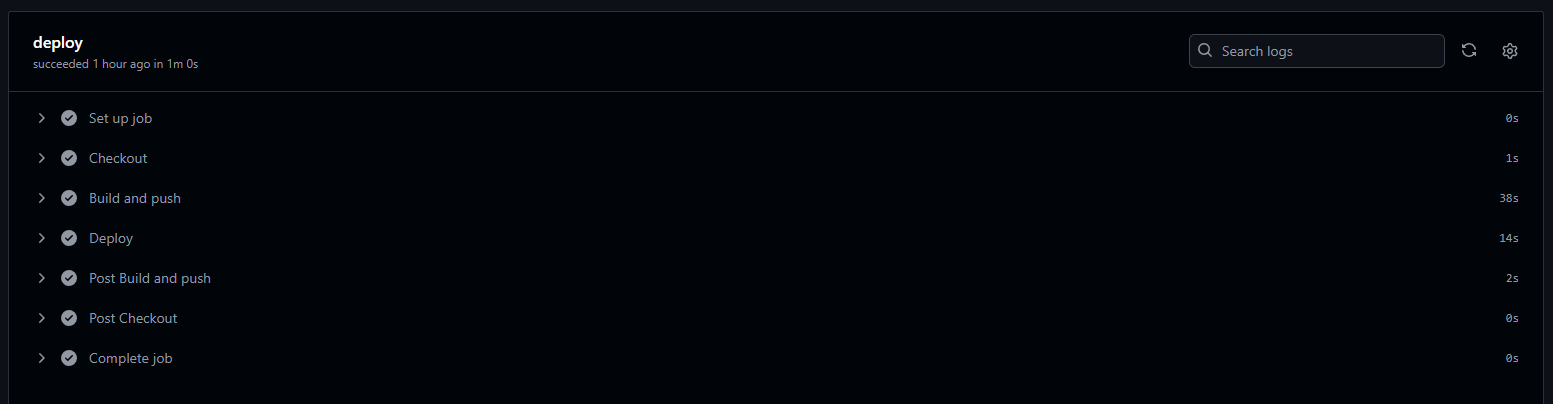
\includegraphics[width=1\linewidth]{pierwszaAkcjaBackendu.png}
    \caption{Rezultat wykonania akcji wdrożenia backendu}
    \label{fig:enter-label}
\end{figure}

W celu przetestowania, czy wszystko działa poprawnie, udałem się pod adres\lstinline|https://ablaszkiewicz.pl/api/counter|. Jak widać na zdjęciu poniżej, wszystko działa poprawnie.

\begin{figure}[H]
    \centering
    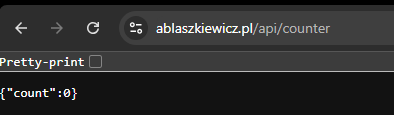
\includegraphics[width=1\linewidth]{rezultatPierwszejWizytyPodBackend.png}
    \caption{Rezultat wejścia na stronę backendu}
    \label{fig:enter-label}
\end{figure}

\subsection{Podsumowanie}

Przeprowadziłem eksperyment i poprosiłem osobę, która nie miała wcześniej styczności z serwerem ani aplikacją, aby wdrożyła ręcznie aplikację na serwer. Zajęło to 7 minut. Dla porównania - automatyczne wdrożenie zajmuje 1 minutę.

\begin{figure}[H]
\centering
\begin{tikzpicture}
\begin{axis}[
    ybar,
    bar width=30pt,
    width=0.6\textwidth, % Zmniejszenie szerokości wykresu
    height=8cm,
    symbolic x coords={Ręczne, Automatyczne},
    xtick=data,
    xlabel={Metoda wdrożenia}, % Dodanie opisu osi X
    ylabel={Czas (minuty)},
    ymin=0,
    ymax=8,
    nodes near coords,
    nodes near coords align={vertical},
    title={Porównanie czasu wdrożenia aplikacji},
    enlarge x limits=0.5, % Wyśrodkowanie słupków
]
\addplot coordinates {(Ręczne,7) (Automatyczne,1)};
\end{axis}
\end{tikzpicture}
\caption{Porównanie czasu potrzebnego do ręcznego i automatycznego wdrożenia aplikacji}
\label{fig:czas_wdrozenia}
\end{figure}

Oprócz tego należy pamiętać, że wspomniana minuta, to nie jest czas dewelopera, w którym podejmuje jakiejś interakcje z infrastrukturą. W czasie wdrażania może robić inne rzeczy. 7 minut w metodzie ręcznej to natomiast czysty czas dewelopera, który musi poświecić na wdrażanie.

\begin{table}[H]
\centering
\begin{tabular}{|l|c|c|}
\hline
\textbf{Cecha} & \textbf{Ręczne wdrożenie} & \textbf{Automatyczne wdrożenie} \\ \hline
Konieczność dzielenia sekretów & \cellcolor{red!50}tak & \cellcolor{green!50}nie \\ \hline
Zajmowanie czasu dewelopera & \cellcolor{red!50}tak & \cellcolor{green!50}nie \\ \hline
Odporność na błędy konfiguracji & \cellcolor{red!50}nie & \cellcolor{green!50}tak \\ \hline
Zduplikowanie podejścia dla innych aplikacji & \cellcolor{red!50}nie & \cellcolor{green!50}tak \\ \hline
\end{tabular}
\caption{Porównanie metod wdrożenia}
\label{tab:porownanie-metod-wdrazania}
\end{table}



\section{Frontend}

W tej sekcji skupię się na konfiguracji pipeline’u dla aplikacji frontendowej, wykorzystując narzędzia
stworzone wcześniej. Jako że użyję tych samych template, to konieczne jest tylko zdefiniowanie
workflow.

\subsection{Workflow}

Znów - poprzednio zdefiniowane template wystarczy teraz tylko wywołać. 

\begin{lstlisting}[caption=Plik \texttt{.github/workflows/prod-deploy-frontend.yml}]
name: Deploy frontend (prod)

on:
  workflow_dispatch:
  push:
    branches:
      - main

jobs:
  deploy:
    runs-on: ubuntu-latest
    steps:
      - name: Checkout
        uses: actions/checkout@v3
      - name: Build and push
        uses: './.github/templates/build-and-push'
        with:
          context: ./frontend
          file: ./frontend/Dockerfile
          dockerhub-username: ${{ secrets.DOCKERHUB_USERNAME }}
          dockerhub-token: ${{ secrets.DOCKERHUB_TOKEN }}
          image-name: ablaszkiewicz/magisterka-frontend-prod
      - name: Deploy
        uses: './.github/templates/deploy-container'
        with:
          host: ${{ secrets.SSH_HOST }}
          username: ${{ secrets.SSH_USER }}
          port: ${{ secrets.SSH_PORT }}
          ssh-private-key: ${{ secrets.SSH_KEY }}
          server-port: 3000
          application-port: 3000
          image-name: ablaszkiewicz/magisterka-frontend-prod
          container-name: magisterka-frontend-prod

\end{lstlisting}

\begin{lstlisting}[caption=Plik \texttt{.github/workflows/dev-deploy-frontend.yml}]
name: Deploy frontend (dev)

on:
  workflow_dispatch:
  push:
    branches:
      - main

jobs:
  deploy:
    runs-on: ubuntu-latest
    steps:
      - name: Checkout
        uses: actions/checkout@v3
      - name: Build and push
        uses: './.github/templates/build-and-push'
        with:
          context: ./frontend
          file: ./frontend/Dockerfile
          dockerhub-username: ${{ secrets.DOCKERHUB_USERNAME }}
          dockerhub-token: ${{ secrets.DOCKERHUB_TOKEN }}
          image-name: ablaszkiewicz/magisterka-frontend-dev
      - name: Deploy
        uses: './.github/templates/deploy-container'
        with:
          host: ${{ secrets.SSH_HOST }}
          username: ${{ secrets.SSH_USER }}
          port: ${{ secrets.SSH_PORT }}
          ssh-private-key: ${{ secrets.SSH_KEY }}
          server-port: 4000
          application-port: 3000
          image-name: ablaszkiewicz/magisterka-frontend-dev
          container-name: magisterka-frontend-dev

\end{lstlisting}

Po wypchnięciu kodu do githuba, akcja włącza się automatycznie.

\begin{figure}[H]
    \centering
    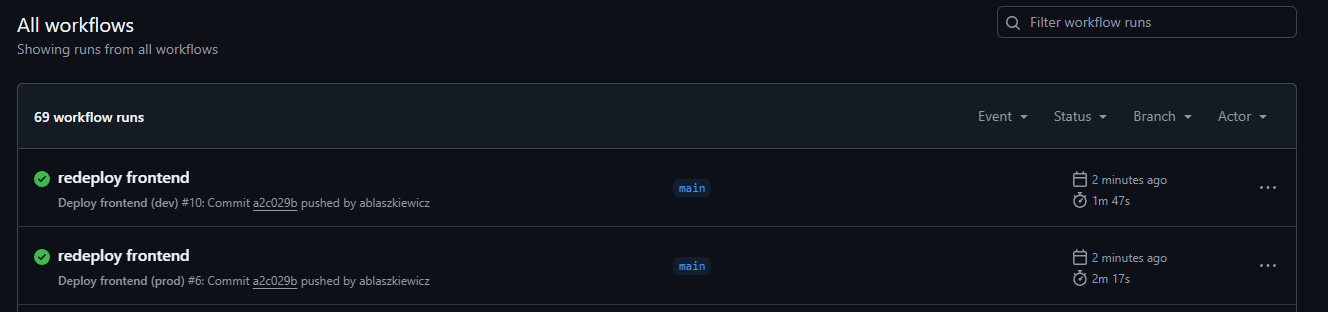
\includegraphics[width=1\linewidth]{rezultatPierwszejAkcjiFrontend.png}
    \caption{Rezultat wdrożenia akcji backendu}
    \label{fig:enter-label}
\end{figure}

W celu przetestowania, czy wszystko działa poprawnie, udałem się pod adres \lstinline|https://ablaszkiewicz.pl|. Jak widać na zdjęciu poniżej, wszystko działa poprawnie. Licznik się aktualizuje.

\begin{figure}[H]
    \centering
    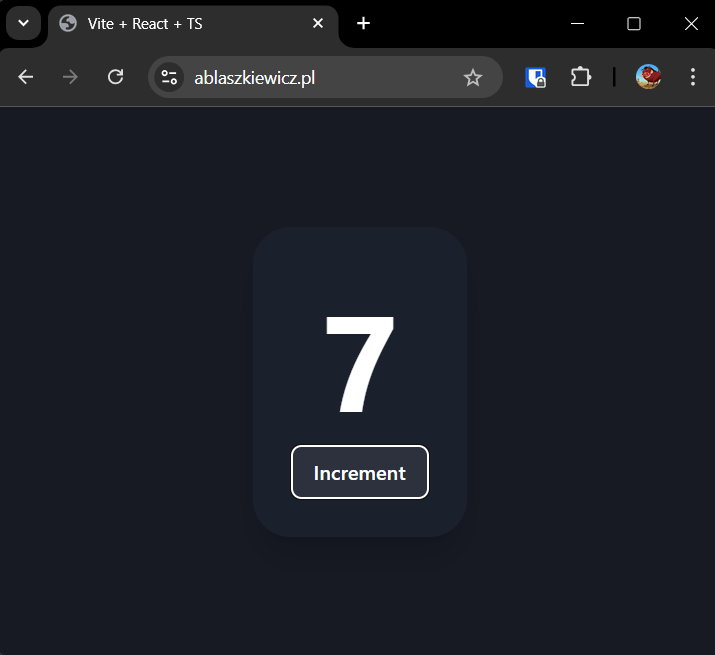
\includegraphics[width=0.5\linewidth]{rezultatWejsciaNaFrontend.png}
    \caption{Rezultat wejścia na stronę frontendu}
    \label{fig:enter-label}
\end{figure}

\section{Podsumowanie dotychczasowej pracy}

Podsumowując, co zrobiłem w poprzednich działach:
\begin{itemize}
    \item zbadanie podejść budowy aplikacji,
    \item zbadanie podejść budowy obrazów,
    \item zbadanie podejść kierowania ruchem,
    \item konfiguracja infrastruktury,
    \item przygotowanie infrastruktury pod wiele środowisk,
    \item dockeryzacja wszystkich aplikacji oraz elementów infrastruktury,
    \item stworzenie reużywalnych templatów,
    \item stworzenie workflow do wszystkich aplikacji oraz elementów infrastruktury.
\end{itemize}

Co w rezultacie daje aplikację, która sama się wdraża na środowisku produkcyjnym przy każdym wypchnięciu kodu na \lstinline|main| oraz na środowisku deweloperskim przy wypchnięciu na \lstinline|dev|.

\begin{figure}[H]
    \centering
    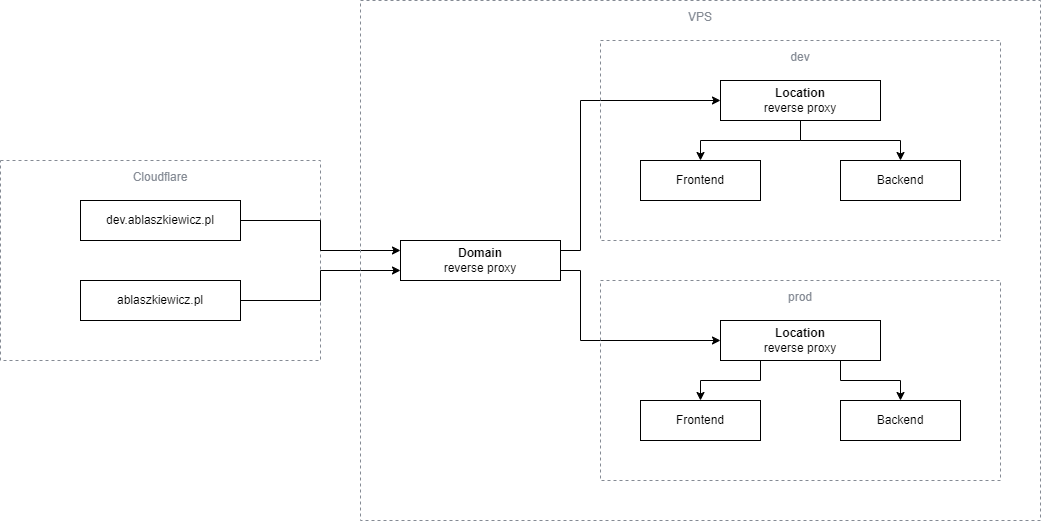
\includegraphics[width=1\linewidth]{diagramInfrasturkturaPolowaPracy.png}
    \caption{Diagram przedstawiający aktualny stan infrastruktury}
    \label{fig:enter-label}
\end{figure}


\section{Observability i monitoring}
\subsection{Co chcę osiągnąć}

W poprzednich rozdziałach skoncentrowałem się na automatyzacji procesów budowania i wdrażania aplikacji, co pozwoliło na efektywne wprowadzenie kultury DevOps do mojego projektu. Jednak jednym z kluczowych elementów tej kultury jest również zapewnienie wysokiego poziomu obserwowalności i monitoringu systemów. Bez odpowiednich narzędzi i mechanizmów monitorujących trudno jest utrzymać stabilność aplikacji oraz szybko reagować na potencjalne problemy.

Celem tego rozdziału jest wprowadzenie rozwiązań, które umożliwią:

\begin{itemize}
    \item \textbf{Monitorowanie stanu serwera} — chcę na bieżąco śledzić takie parametry jak zajętość miejsca na dysku, zużycie pamięci RAM oraz obciążenie procesora CPU. Pozwoli to na szybkie wykrywanie anomalii i zapobieganie awariom wynikającym z braku zasobów,
    \item \textbf{Zbieranie metryk frontendowych} — zależy mi na zrozumieniu interakcji użytkowników z naszą aplikacją. Chcę wiedzieć, ile unikalnych osób odwiedza stronę, z jakich krajów pochodzą oraz jak długo trwa ładowanie poszczególnych komponentów interfejsu,
    \item \textbf{Implementację niestandardowych metryk backendowych} — planuję stworzyć własne metryki, które będą monitorować kluczowe aspekty działania serwera aplikacji, takie jak liczba obsłużonych żądań,
    \item \textbf{Konfigurację systemu alertów} — zależy mi na tym, aby w przypadku wystąpienia krytycznych błędów lub przekroczenia ustalonych progów zużycia zasobów, system automatycznie powiadamiał odpowiednie osoby. Pozwoli to na szybką reakcję i minimalizację potencjalnych strat.
\end{itemize}

Dążę do stworzenia kompleksowego systemu monitoringu, który nie tylko zbierze kluczowe dane, ale również przedstawi je w czytelny i zrozumiały sposób. W ten sposób zwiększymy niezawodność i wydajność naszej aplikacji, a także zapewni lepsze doświadczenia użytkownikom końcowym.

W kolejnych sekcjach dokonam przeglądu dostępnych narzędzi do realizacji tych celów, takich jak Prometheus, Grafana czy Uptime Kuma. Porównam ich możliwości, zalety i wady, a następnie opiszę proces implementacji wybranych rozwiązań w kontekście naszego projektu.

\subsection{Przegląd narzędzi}

\subsubsection{Małe narzędzia}

Małe narzędzia do monitorowania i \textit{observability} są często wybierane w małych projektach ze względu na swoją prostotę, łatwość wdrożenia oraz niskie koszty. Do najpopularniejszych z nich należą:

\begin{itemize}
    \item \textbf{Gatus} – lekki serwer monitorujący, który umożliwia monitorowanie usług poprzez proste konfiguracje w formacie YAML. Oferuje podstawowe powiadomienia i łatwą integrację z istniejącą infrastrukturą. Jest idealny dla prostych zastosowań, gdzie wymagana jest szybka konfiguracja,

\begin{figure}[H]
    \centering
    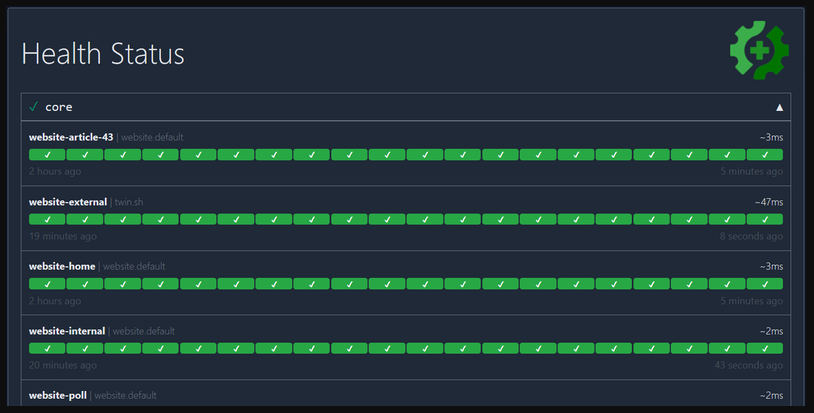
\includegraphics[width=0.5\linewidth]{przykladGatus.png}
    \caption{Przykładowy panel Gatus}
    \label{fig:enter-label}
\end{figure}

    \item \textbf{Uptime Kuma} – przyjazny dla użytkownika monitor serwisów z interfejsem podobnym do Uptime Robot. Pozwala na monitorowanie HTTP(s), TCP, Ping oraz oferuje powiadomienia przez różne kanały, takie jak Telegram czy Slack. Jest łatwy w instalacji i oferuje atrakcyjny interfejs użytkownika,

\begin{figure}[H]
    \centering
    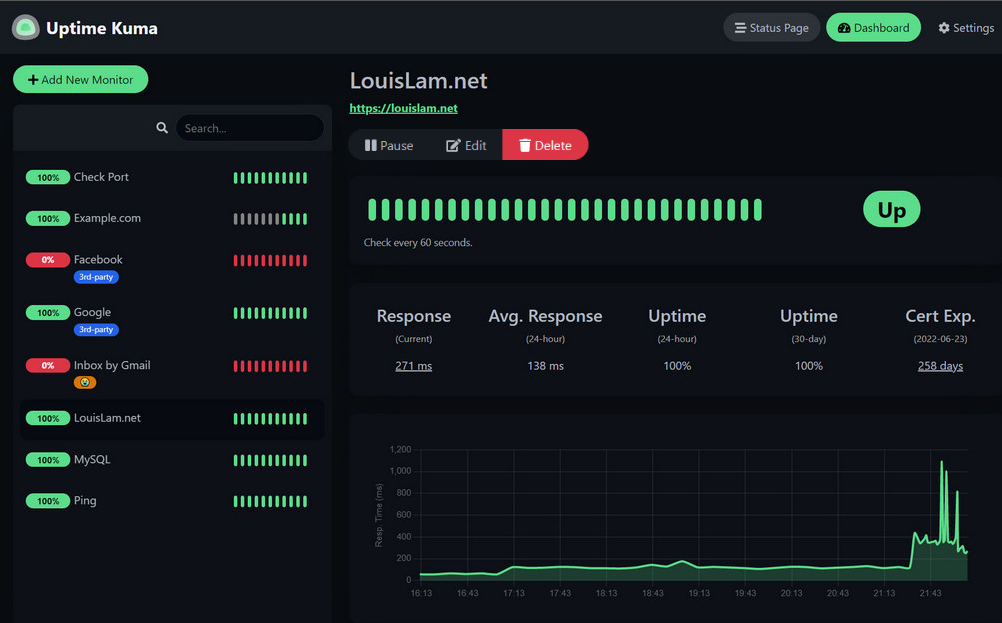
\includegraphics[width=0.5\linewidth]{przykladKuma.png}
    \caption{Przykładowy panel Uptime Kuma}
    \label{fig:enter-label}
\end{figure}

    \item \textbf{Statping} - narzędzie open source do monitorowania statusu usług, które oferuje prosty interfejs i możliwość hostowania własnej strony statusu. Umożliwia monitorowanie usług HTTP(s) i TCP oraz wysyłanie powiadomień. Jest odpowiedni dla małych projektów wymagających podstawowego monitoringu,

\begin{figure}[H]
    \centering
    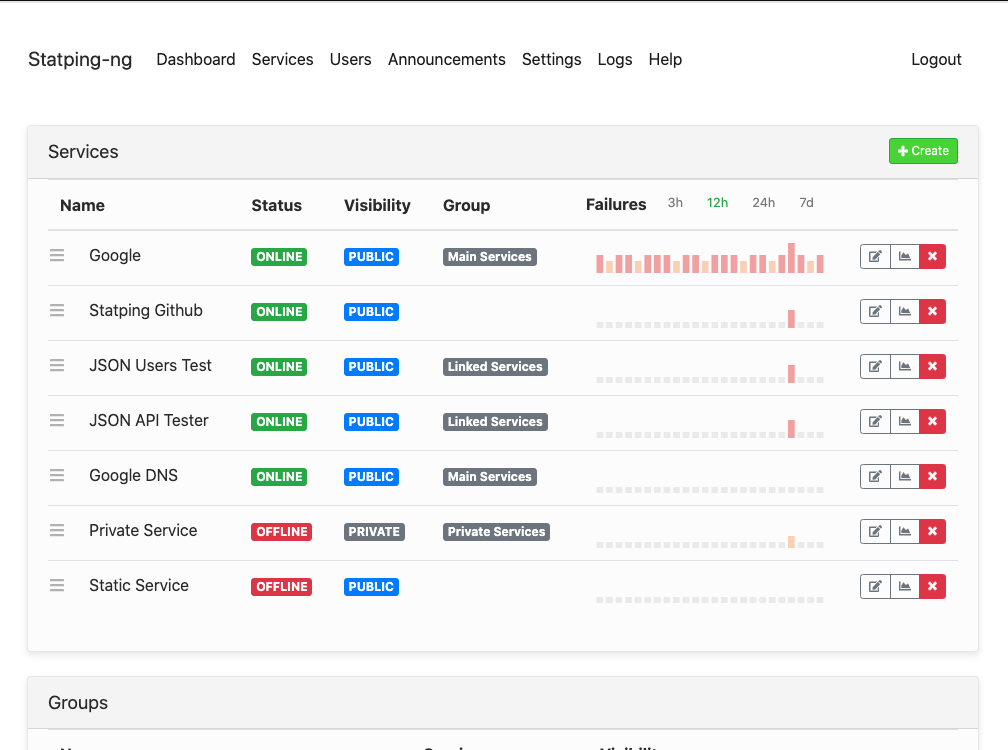
\includegraphics[width=0.5\linewidth]{przykladStatping.png}
    \caption{Przykładowy panel Statping}
    \label{fig:enter-label}
\end{figure}
    
    \item \textbf{Uptime Robot} – popularna usługa SaaS do monitorowania dostępności stron i serwisów. Oferuje darmowy plan z podstawowymi funkcjami oraz płatne plany z dodatkowymi możliwościami i profesjonalnym wsparciem. Dzięki temu jest łatwo dostępny bez konieczności instalacji własnej infrastruktury.

\begin{figure}[H]
    \centering
    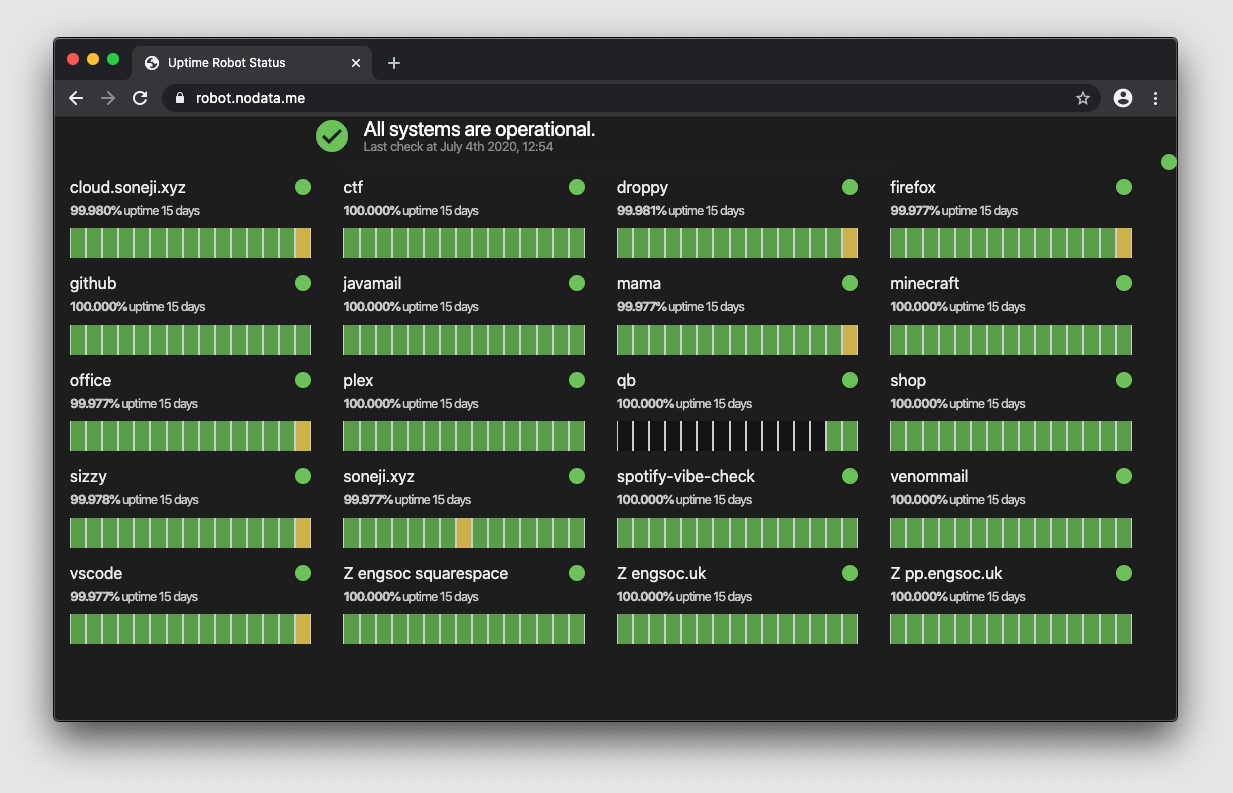
\includegraphics[width=0.5\linewidth]{przykladUptimeRobot.png}
    \caption{Przykładowy panel Uptime Robot}
    \label{fig:enter-label}
\end{figure}
\end{itemize}

\begin{table}[H]
    \centering
    \begin{tabular}{|l|c|c|c|c|}
        \hline
        \textbf{Cecha} & \textbf{Gatus} & \textbf{Uptime Kuma} & \textbf{Statping} & \textbf{Uptime Robot} \\ \hline
        Typ & Open Source & Open Source & Open Source & Usługa SaaS \\ \hline
        Sposób instalacji & Samodzielna & Samodzielna & Samodzielna & Brak instalacji \\ \hline
        Powiadomienia & Tak & Tak & Tak & Tak \\ \hline
        Wspierane protokoły & HTTP, TCP & HTTP(s), TCP, Ping & HTTP(s), TCP & HTTP(s), Ping \\ \hline
        Interfejs użytkownika & Podstawowy & Przyjazny & Podstawowy & Przyjazny \\ \hline
        Skalowalność & Niska & Niska & Niska & Wysoka \\ \hline
        Bezpieczeństwo & Podstawowe & Podstawowe & Podstawowe & Wysokie \\ \hline
        Wsparcie & Społeczność & Społeczność & Społeczność & Profesjonalne \\ \hline
    \end{tabular}
    \caption{Porównanie małych narzędzi monitorujących}
    \label{tab:porownanie-malych-narzedzi}
\end{table}

Małe narzędzia, takie jak wymienione powyżej, są doskonałe dla małych projektów lub indywidualnych potrzeb. Ich zaletą jest prostota oraz możliwość szybkiego wdrożenia bez konieczności angażowania dużych zasobów. Jednak w przypadku projektów o charakterze \textit{enterprise-grade} mogą okazać się niewystarczające.

Często narzędzia te powstawały jako projekty hobbystyczne tworzone przez jedną osobę lub mały zespół. Z tego powodu mogą nie być optymalnie wydajne ani super bezpieczne. Brak regularnych aktualizacji oraz ograniczonego wsparcia mogą 


\subsubsection{Prometheus}

Prometheus jest otwartoźródłowym narzędziem do monitorowania i alertowania, pierwotnie stworzonym w firmie SoundCloud. Obecnie jest rozwijany jako niezależny projekt open source i jest częścią Fundacji Cloud Native Computing Foundation (CNCF). Prometheus został zaprojektowany z myślą o monitorowaniu wysoko dynamicznych środowisk chmurowych.

\begin{figure}[H]
    \centering
    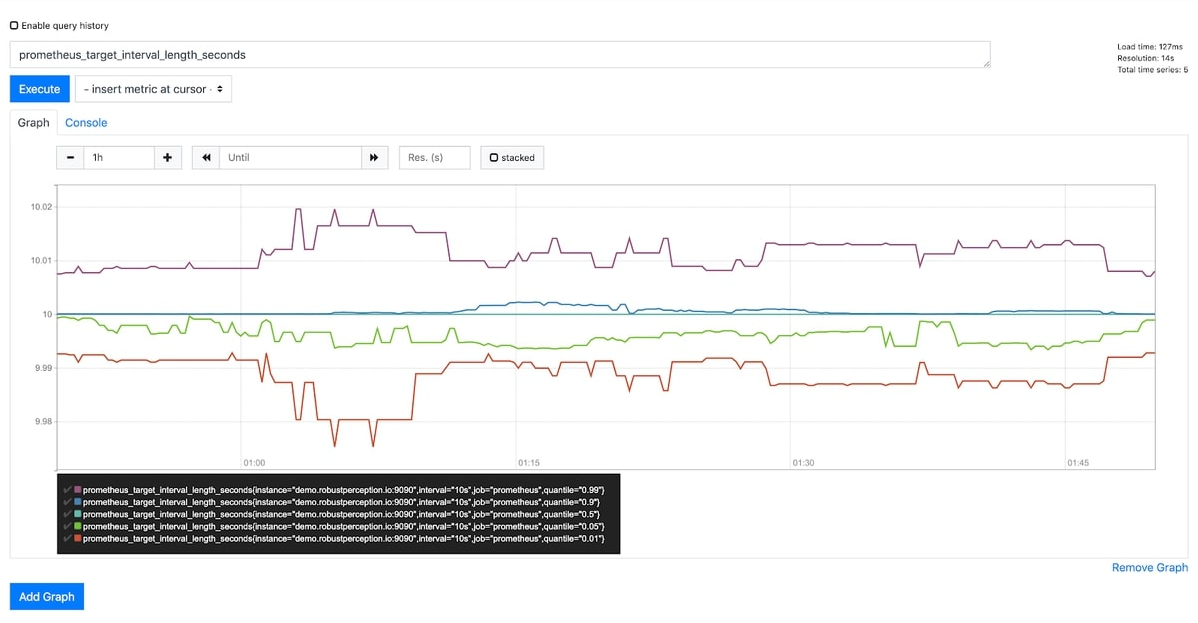
\includegraphics[width=1\linewidth]{prometheusPrzyklad.png}
    \caption{Wynik zapytania o metrykę w panelu Prometheusa}
    \label{fig:enter-label}
\end{figure}

Główne cechy Prometheusa:

\begin{itemize}
    \item \textbf{Model danych oparty na szeregach czasowych} — dane są przechowywane jako szeregi czasowe identyfikowane przez nazwę metryki oraz pary klucz-wartość (tzw. \textit{label}),
    \item \textbf{Język zapytań PromQL} — elastyczny język zapytań umożliwiający agregację i analizę danych,
    \item \textbf{Autonomiczny serwer} — Prometheus nie polega na zewnętrznych systemach przechowywania danych, co zwiększa jego niezawodność,
    \item \textbf{Model pull} — dane są pobierane z monitorowanych usług poprzez HTTP, co ułatwia integrację,
    \item \textbf{Odkrywanie usług} — wsparcie dla dynamicznego odkrywania usług poprzez integracje z systemami takimi jak Kubernetes czy Consul,
    \item \textbf{Alerting} — wbudowany mechanizm alertowania z możliwością integracji z różnymi systemami powiadomień.
\end{itemize}

Prometheus jest idealnym narzędziem dla środowisk \textit{enterprise-grade} ze względu na swoją skalowalność, niezawodność oraz bogaty ekosystem. Pozwala na monitorowanie tysięcy metryk w czasie rzeczywistym, co jest kluczowe w dużych organizacjach. Ponadto, dzięki wsparciu społeczności oraz ciągłemu rozwojowi, Prometheus oferuje aktualne i bezpieczne rozwiązania.

Warto jednak zauważyć, że wdrożenie Prometheusa wymaga pewnej wiedzy i doświadczenia. Konfiguracja może być skomplikowana, a niewłaściwe ustawienia mogą prowadzić do problemów z wydajnością. Dlatego też Prometheus jest często wybierany przez zespoły z odpowiednimi zasobami i kompetencjami technicznymi.

\subsubsection{Grafana}

Grafana to otwartoźródłowa platforma do wizualizacji danych i analizy metryk. Umożliwia tworzenie interaktywnych i dynamicznych dashboardów, które pomagają w monitorowaniu systemów, aplikacji oraz infrastruktury. Grafana integruje się z wieloma źródłami danych, w tym z Prometheusem, Elasticsearch, InfluxDB czy Graphite.

\begin{figure}[H]
    \centering
    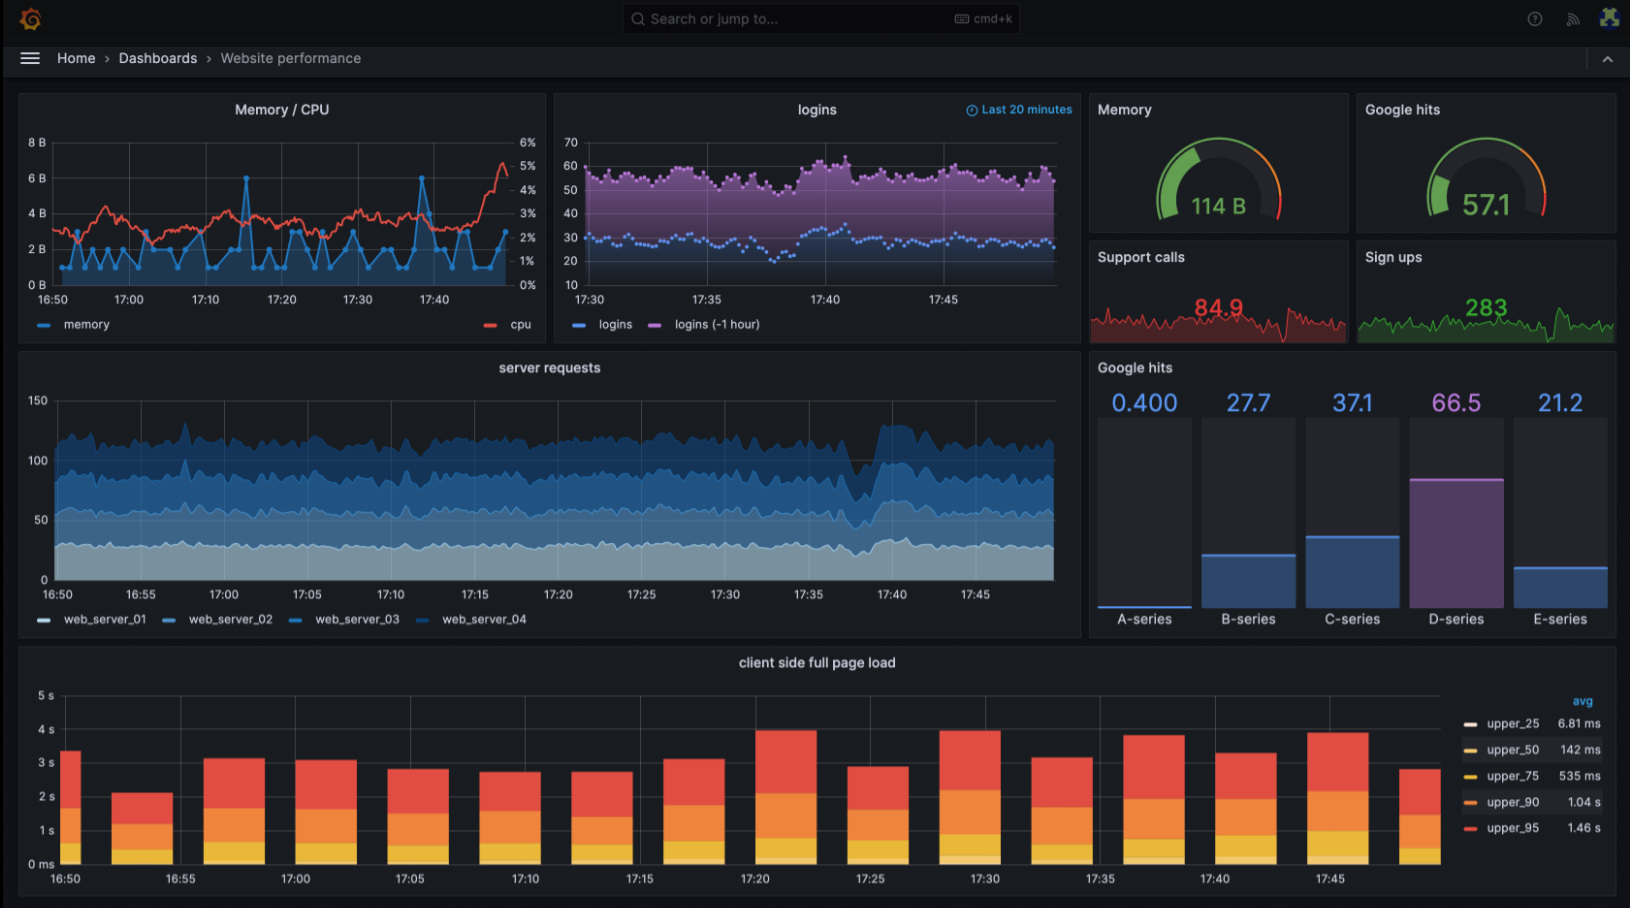
\includegraphics[width=1\linewidth]{grafanaPrzyklad.png}
    \caption{Przykładowy panel w Grafanie}
    \label{fig:enter-label}
\end{figure}

Główne cechy Grafany:

\begin{itemize}
    \item \textbf{Bogate możliwości wizualizacji} — szeroki wybór wykresów, paneli i formatów prezentacji danych,
    \item \textbf{Elastyczność} — możliwość dostosowania dashboardów do indywidualnych potrzeb poprzez edycję paneli i tworzenie własnych wtyczek,
    \item \textbf{Alerting} — wbudowany system alertowania z integracją z różnymi kanałami powiadomień, takimi jak e-mail, Slack czy PagerDuty,
    \item \textbf{Autentykacja i autoryzacja} — wsparcie dla różnych metod uwierzytelniania, w tym LDAP, OAuth czy Grafana Auth,
    \item \textbf{Społeczność i wsparcie} — aktywna społeczność użytkowników oraz regularne aktualizacje i ulepszenia.
\end{itemize}

Grafana jest często wykorzystywana w środowiskach \textit{enterprise-grade} ze względu na swoją skalowalność i możliwości dostosowania. Umożliwia monitorowanie w czasie rzeczywistym oraz analizę historycznych danych, co jest kluczowe dla dużych organizacji. Ponadto, interaktywne dashboardy ułatwiają zrozumienie złożonych zależności i szybkie reagowanie na problemy.

Podobnie jak w przypadku Prometheusa, wdrożenie Grafany może wymagać zaawansowanej wiedzy technicznej. Konfiguracja źródeł danych, tworzenie zaawansowanych dashboardów czy integracja z systemami alertowania może być skomplikowana dla mniej doświadczonych zespołów.

\subsubsection{VictoriaMetrics}

VictoriaMetrics to wysoko wydajny i skalowalny system przechowywania szeregów czasowych oraz narzędzie monitorujące, które jest kompatybilne z ekosystemem Prometheusa. Został stworzony jako odpowiedź na niektóre ograniczenia Prometheusa, szczególnie w kontekście przechowywania długoterminowych danych oraz skalowalności w dużych środowiskach.

\begin{figure}[H]
    \centering
    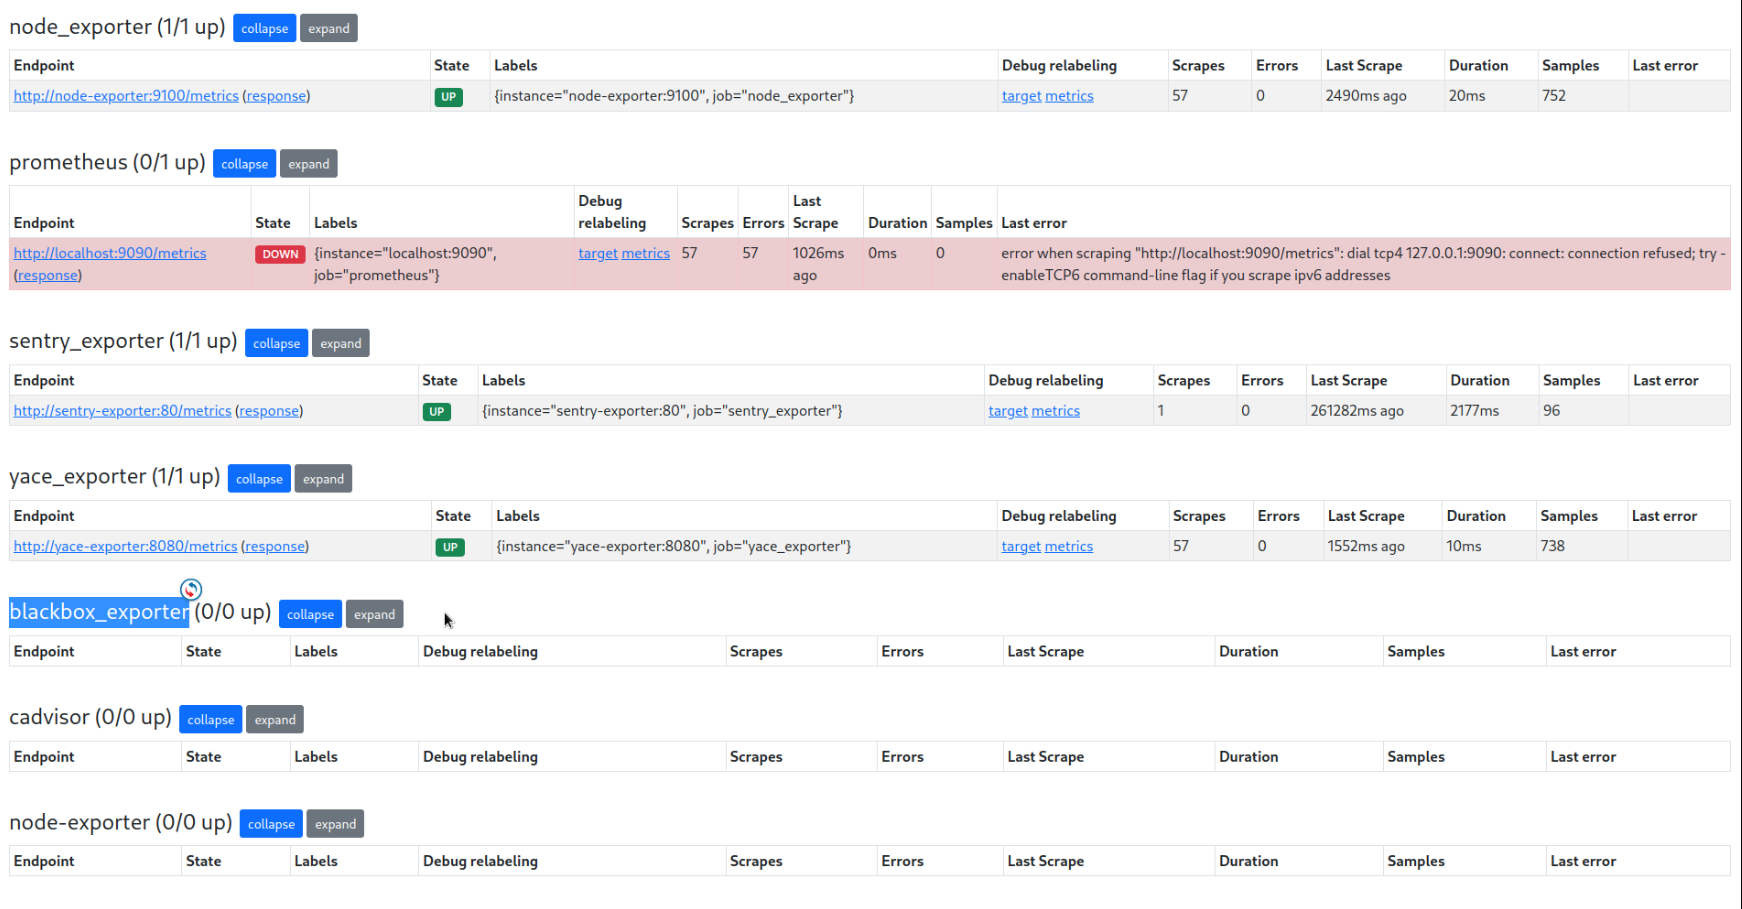
\includegraphics[width=1\linewidth]{victoriaMetricsPrzyklad.png}
    \caption{Przykładowy panel VictoriaMetrics}
    \label{fig:enter-label}
\end{figure}

Główne cechy VictoriaMetrics:

\begin{itemize}
    \item \textbf{Wysoka wydajność i skalowalność} — zaprojektowana do obsługi dużych ilości danych z minimalnym zużyciem zasobów,
    \item \textbf{Kompresja danych} — efektywne algorytmy kompresji, które redukują zużycie przestrzeni dyskowej,
    \item \textbf{Kompatybilność z Prometheusem} — obsługuje protokół zdalnego przechowywania (\textit{Remote Write/Read}), co umożliwia łatwą integrację,
    \item \textbf{Łatwość wdrożenia} — prosty w instalacji i konfiguracji, dostępny jako pojedynczy plik binarny,
    \item \textbf{Wsparcie dla klastrów} — możliwość uruchomienia w trybie klastrowym dla wysokiej dostępności i równoważenia obciążenia.
\end{itemize}

\paragraph{Historia powstania}\mbox{} \\


VictoriaMetrics została stworzona przez zespół inżynierów, którzy zauważyli ograniczenia w istniejących rozwiązaniach do monitorowania i przechowywania danych szeregów czasowych, takich jak Prometheus i InfluxDB. Ich celem było stworzenie narzędzia, które będzie bardziej wydajne pod względem zużycia zasobów oraz lepiej skalowalne w dużych środowiskach.

Pierwsza publiczna wersja VictoriaMetrics została wydana w 2018 roku. Od tego czasu projekt zyskał na popularności wśród firm i organizacji, które potrzebują skalowalnego i wydajnego systemu do monitorowania dużych ilości danych.

\paragraph{Porównanie z Prometheusem}\mbox{} \\


Choć VictoriaMetrics i Prometheus mają wiele wspólnego, istnieją między nimi istotne różnice:

\begin{table}[H]
    \centering
    \begin{tabular}{|l|c|c|}
        \hline
        \textbf{Cecha} & \textbf{Prometheus} & \textbf{VictoriaMetrics} \\ \hline
        Model danych & Szeregi czasowe & Szeregi czasowe \\ \hline
        Skalowalność & Ograniczona & Wysoka \\ \hline
        Długoterminowe przechowywanie & Ograniczone & Efektywne \\ \hline
        Kompresja danych & Podstawowa & Zaawansowana \\ \hline
        Obsługa klastrów & Eksperymentalna & Pełne wsparcie \\ \hline
        Instalacja & Wymaga konfiguracji & Pojedynczy plik binarny \\ \hline
        Ekosystem & Szeroki, duża społeczność & Kompatybilny z Prometheusem \\ \hline
    \end{tabular}
    \caption{Porównanie Prometheusa i VictoriaMetrics}
    \label{tab:porownanie-prometheus-victoriametrics}
\end{table}

\paragraph{Zalety VictoriaMetrics nad Prometheusem:}

\begin{itemize}
    \item \textbf{Lepsza skalowalność} — VictoriaMetrics jest w stanie obsłużyć większe obciążenia przy mniejszym zużyciu zasobów,
    \item \textbf{Efektywne przechowywanie długoterminowe} — dzięki zaawansowanym algorytmom kompresji, VictoriaMetrics jest bardziej efektywna w przechowywaniu danych historycznych,
    \item \textbf{Prostsza instalacja i utrzymanie} — pojedynczy plik binarny ułatwia wdrożenie i zarządzanie,
    \item \textbf{Wsparcie dla klastrów} — wbudowane wsparcie dla uruchamiania w trybie klastrowym.
\end{itemize}

\paragraph{Wady w porównaniu z Prometheusem:}

\begin{itemize}
    \item \textbf{Mniejsza społeczność} — Prometheus ma większą bazę użytkowników i bardziej rozbudowany ekosystem,
    \item \textbf{Mniej wtyczek i integracji} — niektóre narzędzia i wtyczki mogą nie być kompatybilne lub wymagać dodatkowej konfiguracji,
    \item \textbf{Mniejsza elastyczność w niektórych obszarach} — niektóre zaawansowane funkcje Prometheusa mogą być trudniejsze do zaimplementowania w VictoriaMetrics.
\end{itemize}


VictoriaMetrics jest potężnym narzędziem dla organizacji, które potrzebują skalowalnego i wydajnego systemu monitorowania z możliwością długoterminowego przechowywania danych. Dzięki kompatybilności z ekosystemem Prometheusa, migracja lub integracja jest stosunkowo prosta. Jednak wybór pomiędzy Prometheusem a VictoriaMetrics zależy od konkretnych potrzeb i zasobów organizacji. Prometheus może być lepszym wyborem dla środowisk z mniejszymi wymaganiami skalowalności i potrzebą korzystania z szerokiego ekosystemu narzędzi i wtyczek.

\subsubsection{Podsumowanie}

Prometheus i Grafana to potężne narzędzia, które w połączeniu oferują kompleksowe rozwiązanie do monitorowania i wizualizacji danych w środowiskach o wysokich wymaganiach. Są one znacznie bardziej zaawansowane niż małe narzędzia omówione wcześniej i są odpowiednie dla projektów \textit{enterprise-grade}.

Ich wdrożenie i utrzymanie wymaga jednak większych zasobów oraz wiedzy technicznej. W zamian oferują skalowalność, wydajność oraz szerokie możliwości dostosowania, co sprawia, że są preferowanym wyborem w dużych organizacjach, gdzie niezawodność i bezpieczeństwo są priorytetem.

\subsection{Provisioning}

Tak, jak dotychczas w tej pracy opisywałem proces automatyzacji wdrażania i konfiguracji poszczególnych narzędzi, tak też będę robił w przypadku infrastruktury. W tym przypadku monitoringu to podejście nie jest oczywiste i w przypadku każdego narzędzia będą występowały różnice, jednak twórcy takich rozwiązań są świadomi potrzeb i większość narzędzi jest do tego przystosowana.

Ominę kroki ręcznego wdrażania i przejdę po prostu do wdrażania za pomocą zautomatyzowanych akcji.

\subsection{Implementacja}

\subsubsection{Node Exporter}

Node Exporter to narzędzie stworzone specjalnie do monitorowania serwera. Zbierane metryki obejmują zasoby sprzętowe, takie jak procesor, pamięć RAM, przestrzeń dyskową, oraz inne parametry systemowe. W celu integracji Node Exportera z Prometheusem i wdrożenia go na serwerze, wystarczy uruchomić go w kontenerze.

Stworzyłem pomocniczy template, który stopuje stare kontenery na podstawie listy nazw oddzielonych przecinkiem dostarczonych jako parametr.

\begin{lstlisting}[caption=Plik \texttt{.github/templates/stop-old-containers/action.yml}]
name: Stop old containers

inputs:
  # ssh
  ssh-host:
    required: true
  ssh-username:
    required: true
  ssh-port:
    required: true
  ssh-key:
    required: true

  names:
    required: true

runs:
  using: 'composite'
  steps:
    - name: Stop old containers
      uses: appleboy/ssh-action@master
      with:
        host: ${{ inputs.ssh-host }}
        USERNAME: ${{ inputs.ssh-username }}
        PORT: ${{ inputs.ssh-port }}
        KEY: ${{ inputs.ssh-key }}
        script: |
          IFS=',' read -r -a container_names <<< "${{ inputs.names }}"

          # Loop through each container name in the array
          for container in "${container_names[@]}"
          do
              echo "Stopping and removing containers with exact name: $container"

              # Find container IDs with exact name match
              container_ids=$(docker ps -aq --filter "name=^${container}$")

              if [ ! -z "$container_ids" ]; then
                  echo "Containers found for ${container}, stopping and removing..."
                  docker stop $container_ids
                  docker rm $container_ids
              else
                  echo "No containers found with the exact name: $container"
              fi
          done
\end{lstlisting}

Następnie stworzyłem template, który włączy Node Exportera z potrzebnymi flagami. Nadają one Node Exporterowi szerokie uprawnienia, a to dlatego, że działa on w warstwie hosta.

\begin{lstlisting}[caption=Plik \texttt{.github/templates/deploy-node-exporter/action.yml}]
name: Deploy node exporter

inputs:
  # ssh
  ssh-host:
    required: true
  ssh-username:
    required: true
  ssh-port:
    required: true
  ssh-key:
    required: true

runs:
  using: 'composite'
  steps:
    - name: Deploy node exporter
      uses: appleboy/ssh-action@master
      with:
        host: ${{ inputs.ssh-host }}
        USERNAME: ${{ inputs.ssh-username }}
        PORT: ${{ inputs.ssh-port }}
        KEY: ${{ inputs.ssh-key }}
        script: |
          docker run -d \
          --name="monitoring-node-exporter" \
          --net="host" \
          --pid="host" \
          -v "/:/host:ro,rslave" \
          --restart=always \
          quay.io/prometheus/node-exporter:v1.7.0 \
          --path.rootfs=/host
\end{lstlisting}

Na koniec stworzyłem workflow, który skorzysta z wcześniej stworzonych templatów.

\begin{lstlisting}[caption=Plik \texttt{.github/workflows/prod-deploy-node-exporter.yml}]
name: Deploy node exporter (prod)
on:
  workflow_dispatch: null
  push:
    branches:
      - main
jobs:
  deploy:
    runs-on: ubuntu-latest
    steps:
      - name: Checkout
        uses: actions/checkout@v3
      - name: Stop old containers
        uses: ./.github/templates/stop-old-containers
        with:
          ssh-host: ${{ secrets.SSH_HOST }}
          ssh-username: ${{ secrets.SSH_USER }}
          ssh-port: ${{ secrets.SSH_PORT }}
          ssh-key: ${{ secrets.SSH_KEY }}
          names: 'monitoring-node-exporter'
      - name: Deploy node exporter
        uses: ./.github/templates/deploy-node-exporter
        with:
          ssh-host: ${{ secrets.SSH_HOST }}
          ssh-username: ${{ secrets.SSH_USER }}
          ssh-port: ${{ secrets.SSH_PORT }}
          ssh-key: ${{ secrets.SSH_KEY }}

\end{lstlisting}

Weryfikację poprawności wdrożenia dokonałem poprzez wykonanie \lstinline|curl localhost:9100/metrics|.

\begin{figure}[H]
    \centering
    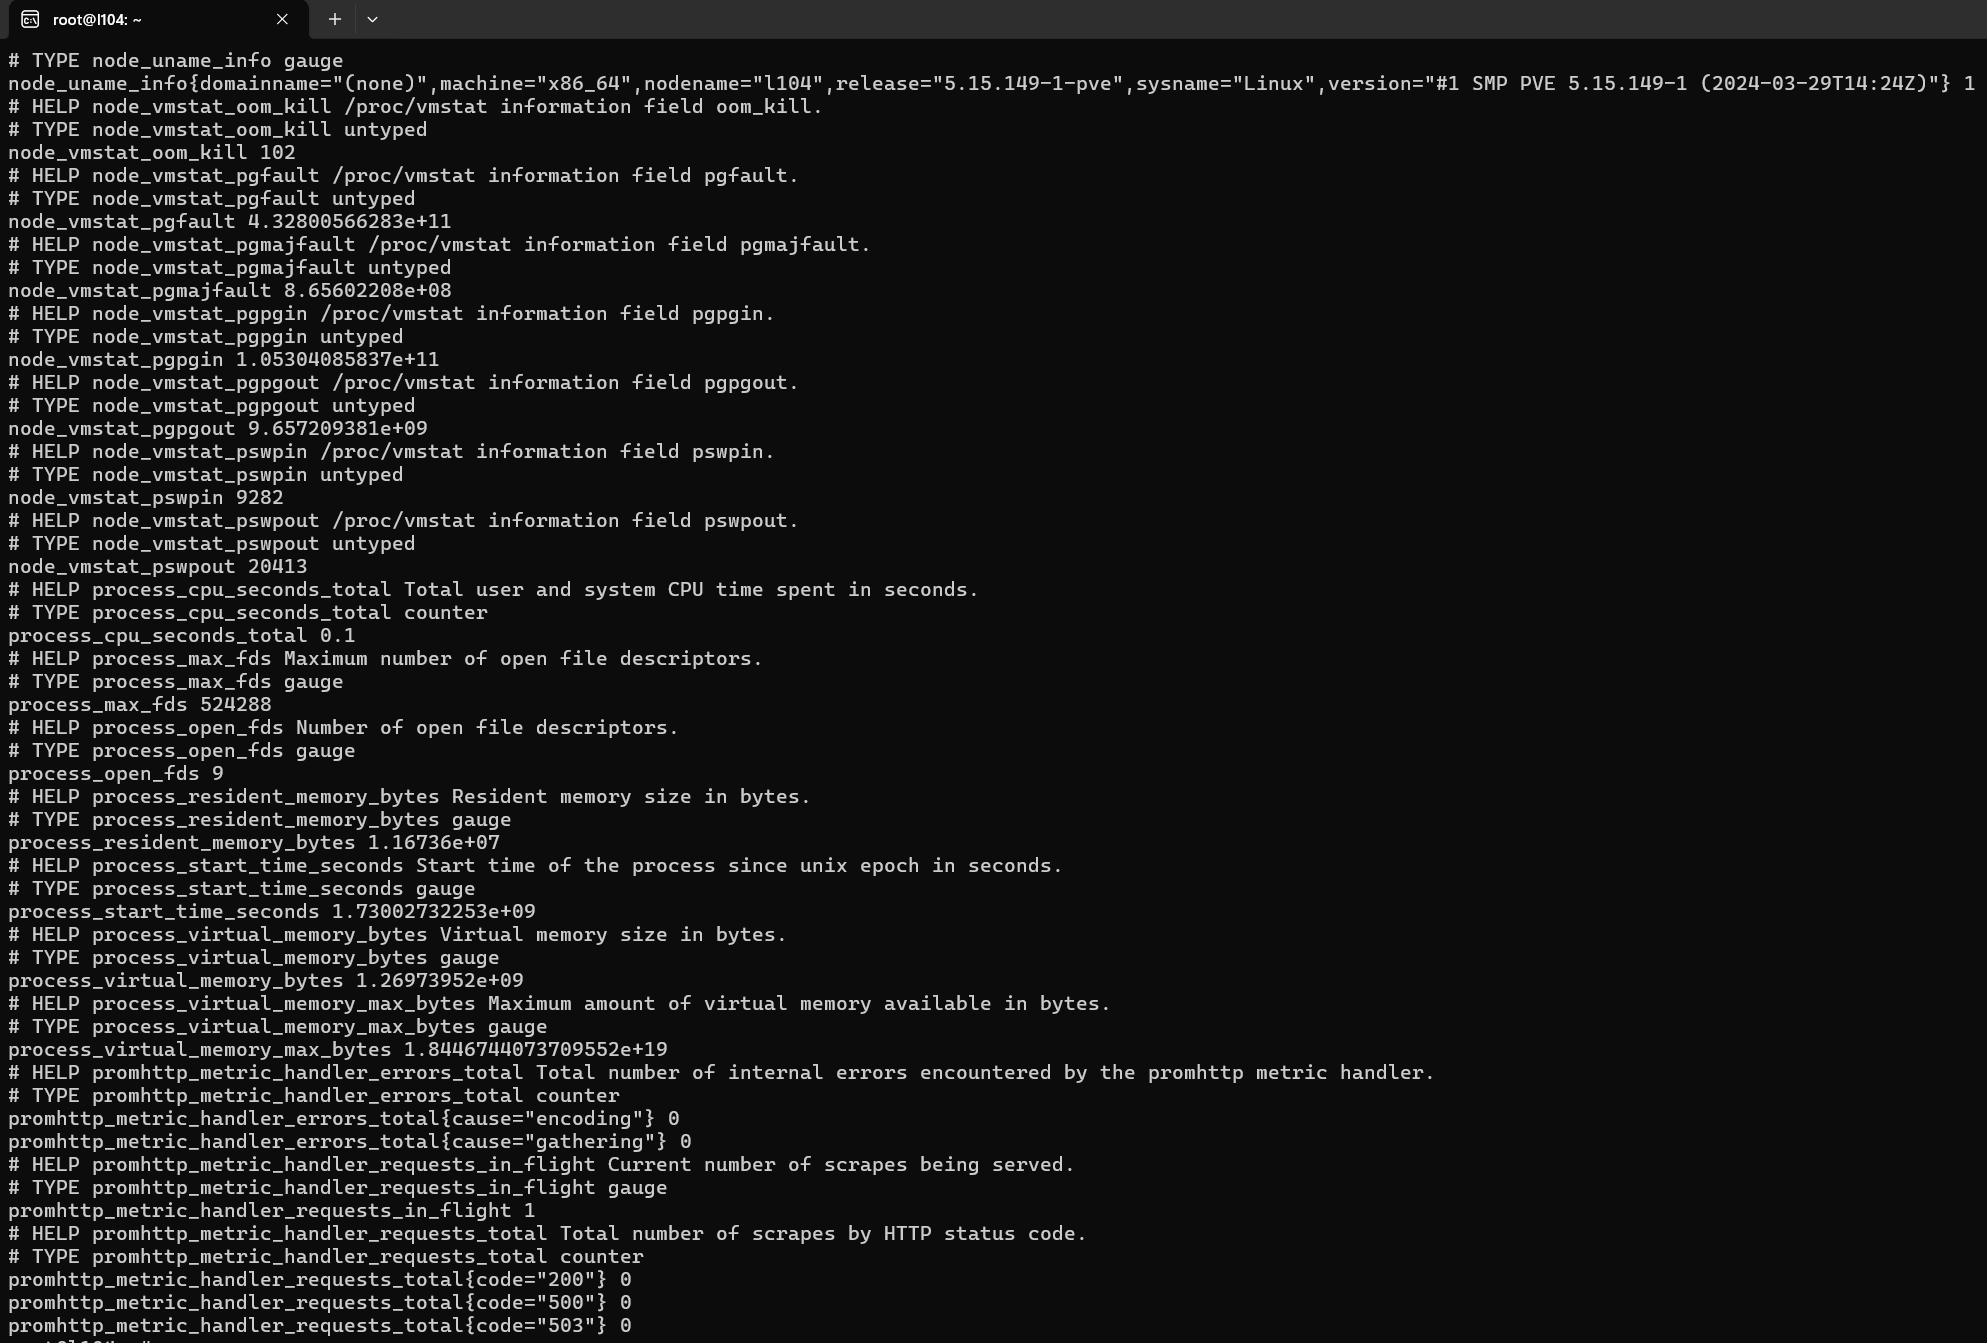
\includegraphics[width=0.75\linewidth]{metrykiNodeExporterRaw.png}
    \caption{Weryfikacja poprawności działania Node Exportera}
    \label{fig:enter-label}
\end{figure}

\subsubsection{Prometheus}

Narzędziem, które będzie zbierało metryki produkowane przez Node Exportera jest Prometheus. Konfiguracja narzędzia odbywa się poprzez plik \lstinline|.yaml|.

Pomysł na automatyczną konfigurację tego narzędzia jest taki, że plik konfiguracyjny będzie znajdował się w repozytorium z infrastrukturą. Całe repozytorium zostanie pobrane do specjalnie utworzonego katalogu na serwerze i w momencie włączania Prometheusa zamontuję ten plik jako \textbf{volume} i podam odpowiedni argument.

\begin{figure}[H]
    \centering
    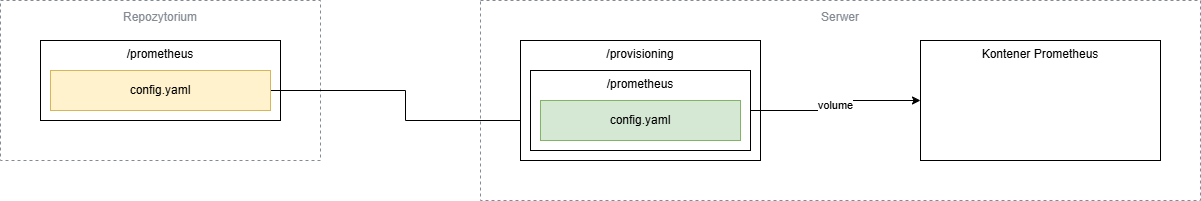
\includegraphics[width=1\linewidth]{diagramProvisionPrometheus.png}
    \caption{Diagram przedstawiający strategię provisioningu Prometheusa}
    \label{fig:enter-label}
\end{figure}

Zacząłem od stworzenia wspomnianego pliku konfiguracyjnego. Określa się w nim, pod jakimi adresami dostępne są metryki. Dodatkowo możliwe jest ustawienie częstotliwości zbierania metryk oraz nadanie im nazw.

W tym przypadku Prometheus będzie posiadał tylko jeden job i będzie nim zbieranie metryk Node Exportera.

\begin{lstlisting}[caption=Plik \texttt{infrastructure/prometheus/prometheus.yml}]
global:
  scrape_interval: 5s
  external_labels:
    monitor: 'node'
scrape_configs:
  - job_name: 'node-exporter'
    static_configs:
      - targets: ['host.docker.internal:9100']

\end{lstlisting}

Następnie stworzyłem template, który kolejno:
\begin{itemize}
    \item stworzy specjalny katalog na rzeczy związane z Prometheusem,
    \item wejdzie do niego,
    \item pobierze repozytorium git,
    \item włączy kontener montując plik konfiguracyjny prometheusa jako volume.
\end{itemize}

\begin{lstlisting}[caption=Plik \texttt{.github/templates/deploy-prometheus/action.yml}]
name: Deploy prometheus

inputs:
  # ssh
  ssh-host:
    required: true
  ssh-username:
    required: true
  ssh-port:
    required: true
  ssh-key:
    required: true

runs:
  using: 'composite'
  steps:
    - name: Deploy prometheus
      uses: appleboy/ssh-action@master
      with:
        host: ${{ inputs.ssh-host }}
        USERNAME: ${{ inputs.ssh-username }}
        PORT: ${{ inputs.ssh-port }}
        KEY: ${{ inputs.ssh-key }}
        script: |
          rm -rf ~/provisioning/prometheus
          mkdir -p ~/provisioning/prometheus
          cd ~/provisioning/prometheus
          git clone https://github.com/ablaszkiewicz/devops-sandbox.git
          cd devops-sandbox/infrastructure/prometheus

          docker run -d \
          --name="monitoring-prometheus" \
          --add-host=host.docker.internal:host-gateway \
          -p 9090:9090 \
          -v $PWD/prometheus.yml:/etc/prometheus/prometheus.yml \
          --restart=always \
          prom/prometheus:v2.49.1
\end{lstlisting}

Na końcu stworzyłem workflow, który skorzysta z wcześniej stworzonego template.

\begin{lstlisting}[caption=Plik \texttt{.github/workflows/prod-deploy-prometheus.yml}]
name: Deploy prometheus (prod)
on:
  workflow_dispatch: null
  push:
    branches:
      - never
jobs:
  deploy:
    runs-on: ubuntu-latest
    steps:
      - name: Checkout
        uses: actions/checkout@v3
      - name: Stop old containers
        uses: ./.github/templates/stop-old-containers
        with:
          ssh-host: ${{ secrets.SSH_HOST }}
          ssh-username: ${{ secrets.SSH_USER }}
          ssh-port: ${{ secrets.SSH_PORT }}
          ssh-key: ${{ secrets.SSH_KEY }}
          names: 'monitoring-prometheus'
      - name: Deploy prometheus
        uses: ./.github/templates/deploy-prometheus
        with:
          ssh-host: ${{ secrets.SSH_HOST }}
          ssh-username: ${{ secrets.SSH_USER }}
          ssh-port: ${{ secrets.SSH_PORT }}
          ssh-key: ${{ secrets.SSH_KEY }}

\end{lstlisting}

Aby przetestować poprawność konfiguracji mogę użyć komendy \lstinline|ssh -L 9090:localhost:9090 magisterka|, aby przekierować ruch portu \textbf{Prometheusa} na moją lokalną maszynę, po czym mogę odwiedzić \lstinline|http://localhost:9090/targets|, aby zobaczyć skonfigurowane cele.

\begin{figure}[H]
    \centering
    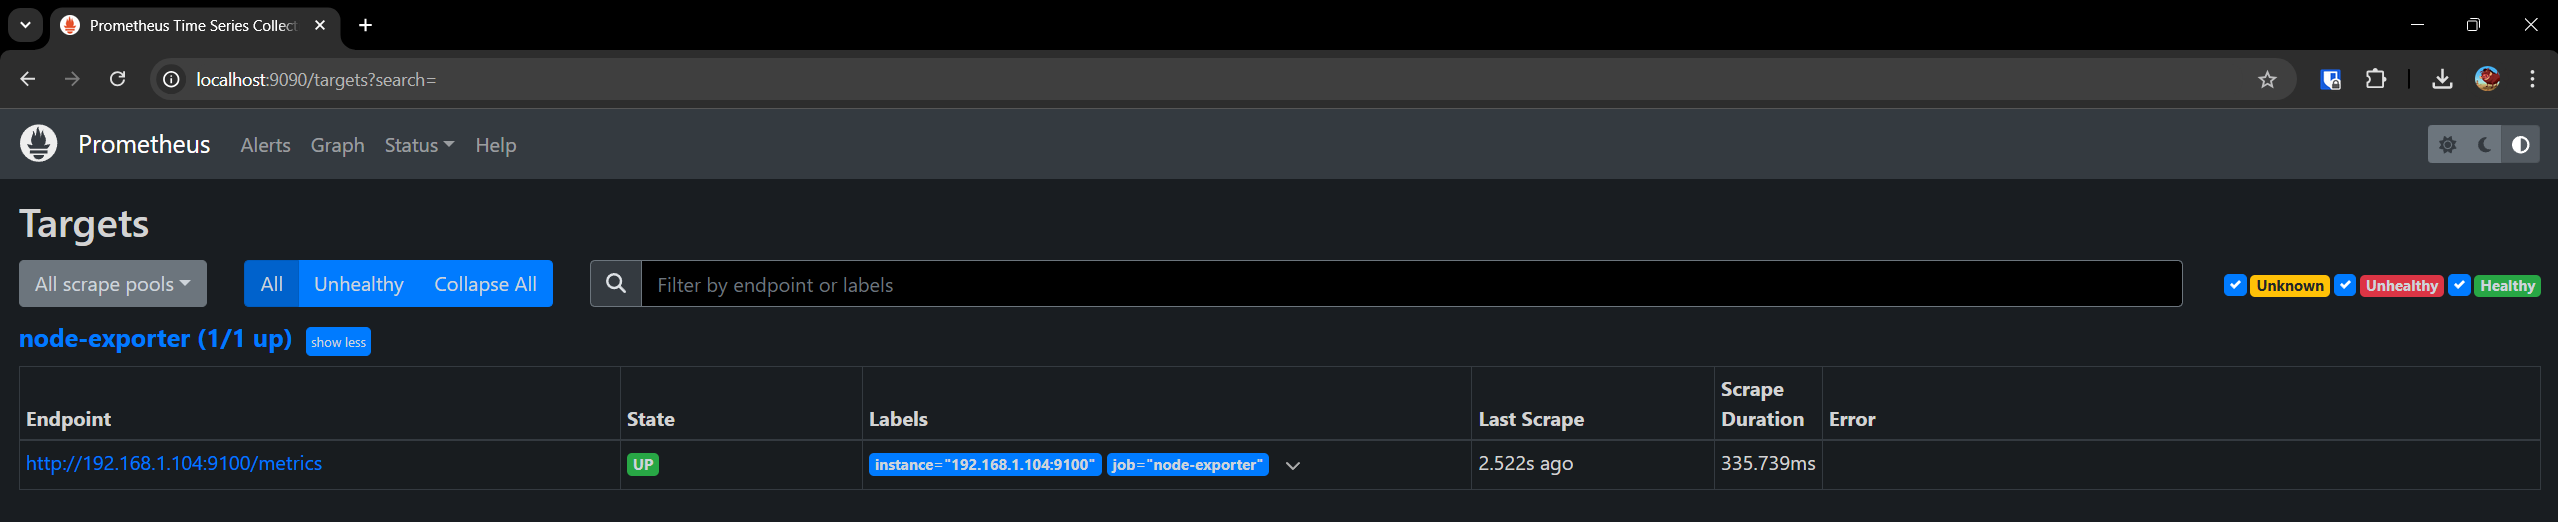
\includegraphics[width=1\linewidth]{prometheusSprawdzenieKonfiguracji.png}
    \caption{Skonfigurowane cele scrapowania w panelu Prometheus}
    \label{fig:enter-label}
\end{figure}

Na rysunku widać, że \textbf{Prometheus} poprawnie scrapuje dane z \textbf{Node Exportera}

\subsubsection{Grafana}

Grafana jest narzędziem wizualizacyjnym, które umożliwia przeglądanie i analizowanie danych zbieranych przez Prometheusa. Dzięki integracji z Prometheusem użytkownik może z łatwością tworzyć zaawansowane panele do wizualizacji danych.

Stworzyłem template, który włącza kontener z Grafaną.

\begin{lstlisting}[caption=Plik \texttt{.github/templates/deploy-grafana/action.yml}]
name: Deploy grafana

inputs:
  ssh-host:
    required: true
  ssh-username:
    required: true
  ssh-port:
    required: true
  ssh-key:
    required: true

  grafana-username:
    required: true
  grafana-password:
    required: true

runs:
  using: 'composite'
  steps:
    - name: Deploy grafana
      uses: appleboy/ssh-action@master
      with:
        host: ${{ inputs.ssh-host }}
        USERNAME: ${{ inputs.ssh-username }}
        PORT: ${{ inputs.ssh-port }}
        KEY: ${{ inputs.ssh-key }}
        script: |
          docker run \
            -d \
            -p 2000:3000 \
            --add-host=host.docker.internal:host-gateway \
            --name=monitoring-grafana \
            -e "GF_SECURITY_ADMIN_USER=${{ inputs.grafana-username }}" \
            -e "GF_SECURITY_ADMIN_PASSWORD=${{ inputs.grafana-password }}" \
            --restart=always \
            grafana/grafana:10.3.3
\end{lstlisting}

Dodatkowo stworzyłem workflow, który korzysta z dwóch poprzednich plików.

\begin{lstlisting}[caption=Plik \texttt{.github/workflows/prod-deploy-grafana.yml}]
name: Deploy grafana (prod)
on:
  workflow_dispatch: null
  push:
    branches:
      - main
jobs:
  deploy:
    runs-on: ubuntu-latest
    steps:
      - name: Checkout
        uses: actions/checkout@v3
      - name: Stop old containers
        uses: ./.github/templates/stop-old-containers
        with:
          ssh-host: ${{ secrets.SSH_HOST }}
          ssh-username: ${{ secrets.SSH_USER }}
          ssh-port: ${{ secrets.SSH_PORT }}
          ssh-key: ${{ secrets.SSH_KEY }}
          names: 'monitoring-grafana'
      - name: Deploy grafana
        uses: ./.github/templates/deploy-grafana
        with:
          ssh-host: ${{ secrets.SSH_HOST }}
          ssh-username: ${{ secrets.SSH_USER }}
          ssh-port: ${{ secrets.SSH_PORT }}
          ssh-key: ${{ secrets.SSH_KEY }}
          grafana-username: ${{ secrets.MONITORING_USERNAME }}
          grafana-password: ${{ secrets.MONITORING_PASSWORD }}
\end{lstlisting}

Pozostało stworzyć sekrety w repozytorium.

\begin{figure}[H]
    \centering
    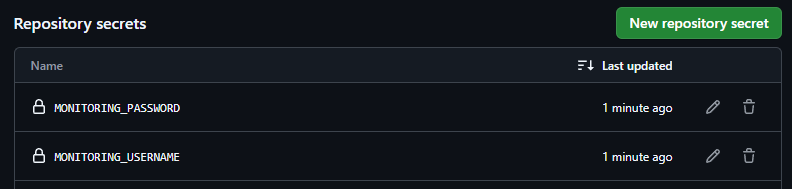
\includegraphics[width=1\linewidth]{sekretyGrafana.png}
    \caption{Sekrety uwierzytelniania do grafany dodane do repozytorium}
    \label{fig:enter-label}
\end{figure}

Oraz podłączyć domenę w cloudflare.

\begin{figure}[H]
    \centering
    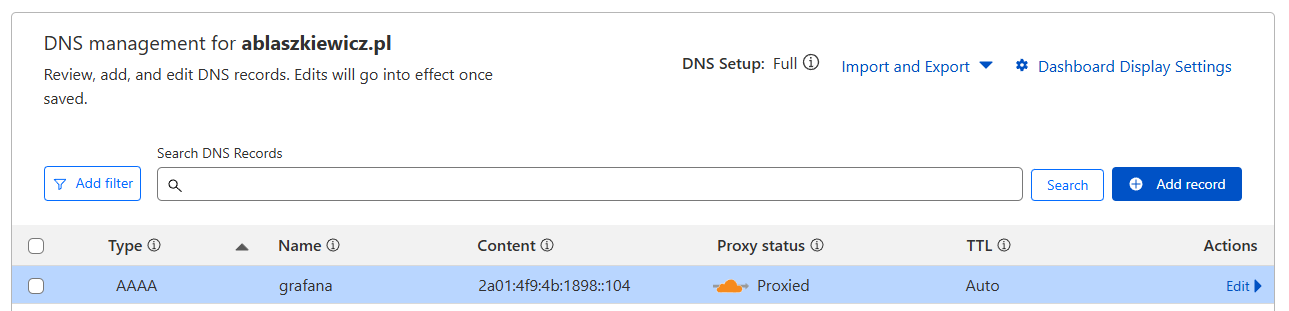
\includegraphics[width=1\linewidth]{grafanaDNS.png}
    \caption{Ustawienia DNS Grafana}
    \label{fig:enter-label}
\end{figure}

I na koniec zmienić konfigurację wcześniej stworzonego współdzielonego reverse proxy tak, aby ruch z \lstinline|grafana.ablaszkiewicz.pl| kierował na \lstinline|localhost:2000|, na którym zostanie wdrożona Grafana.

\begin{lstlisting}[caption=Zaktualizowany plik \texttt{infrastructure/reverse-proxy-shared/config}]
grafana.ablaszkiewicz.pl=http://192.168.1.104:2000
dev.ablaszkiewicz.pl=http://192.168.1.104:4080
ablaszkiewicz.pl=http://192.168.1.104:3080
\end{lstlisting}

Po konfiguracji jestem w stanie wejść na stronę swojej grafany.

\begin{figure}[H]
    \centering
    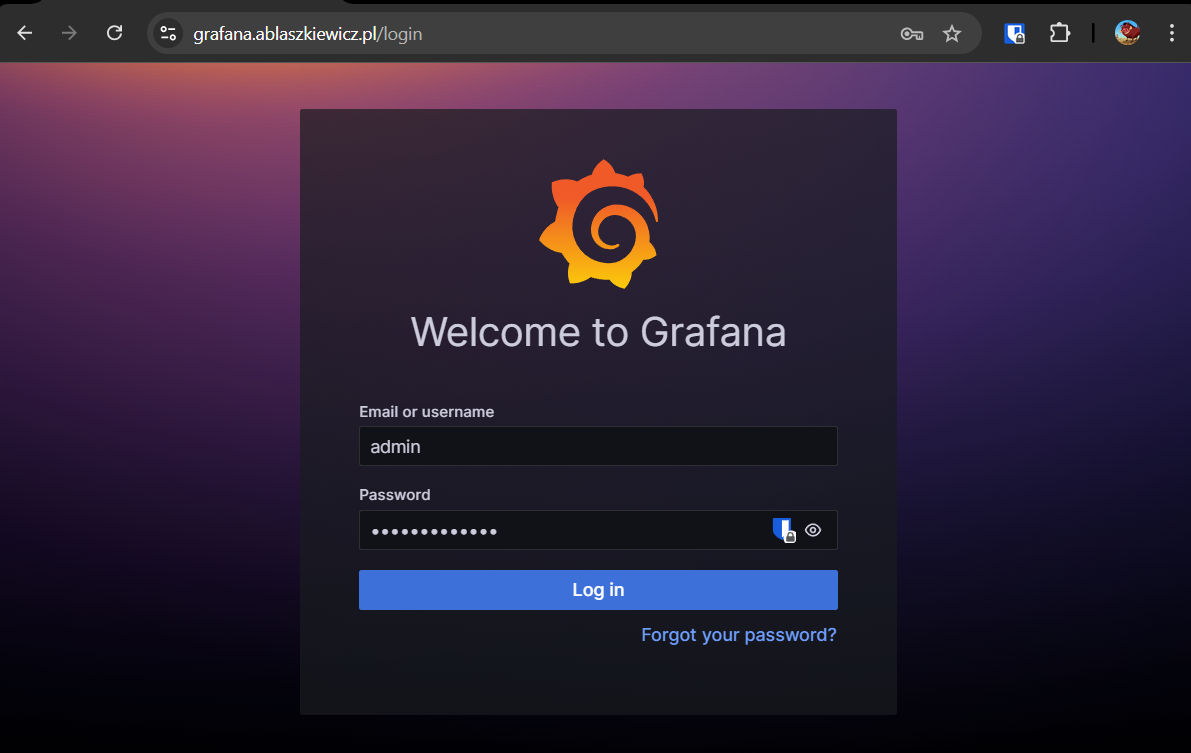
\includegraphics[width=0.75\linewidth]{grafanaLogowanie.png}
    \caption{Odwiedzenie adresu Grafany}
    \label{fig:enter-label}
\end{figure}

Pomyślnie loguje się zapisanymi w sekretach danymi.

\begin{figure}[H]
    \centering
    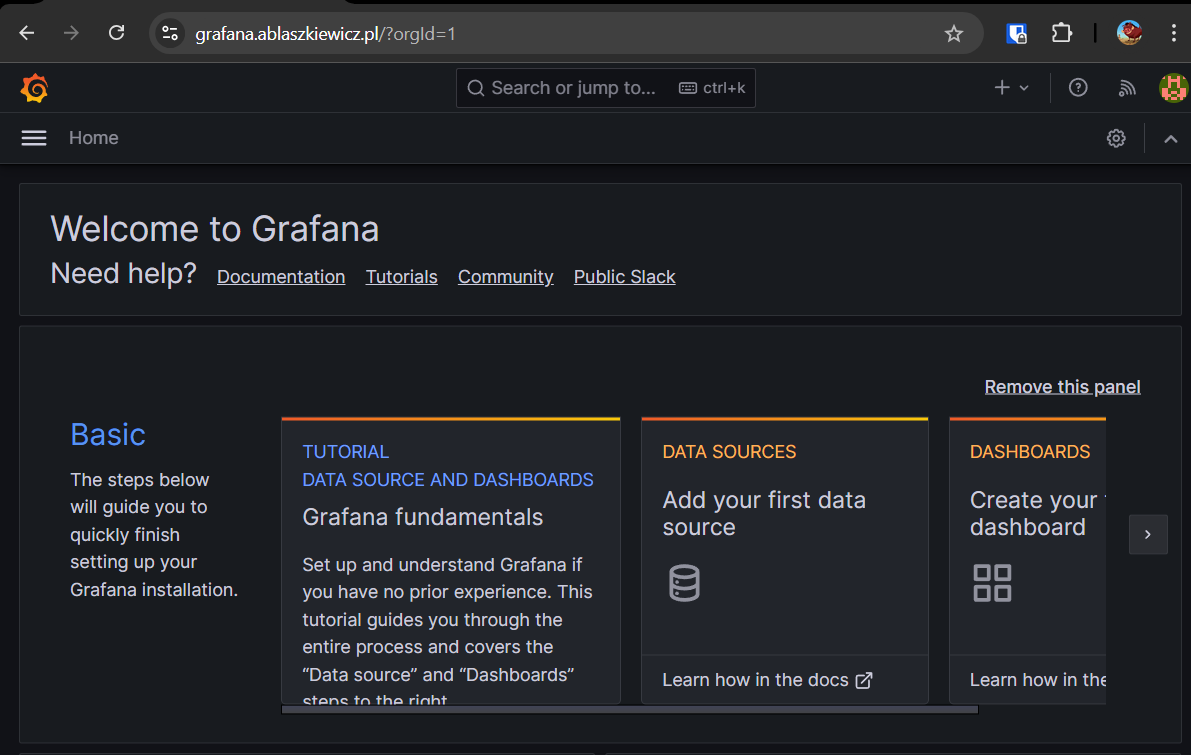
\includegraphics[width=0.75\linewidth]{grafanaPomyslneZalogowanie.png}
    \caption{Pomyślne zalogowanie do Grafany}
    \label{fig:enter-label}
\end{figure}

Aby zweryfikować poprawność działania poprzednich kroków, spróbuję dodać \textbf{Prometheusa} jako \textbf{Data Srouce}. W tym celu udałem się do zakładki Data Sources i po kliknięciu Add data source wpisałem adres prometheusa

\begin{figure}[H]
    \centering
    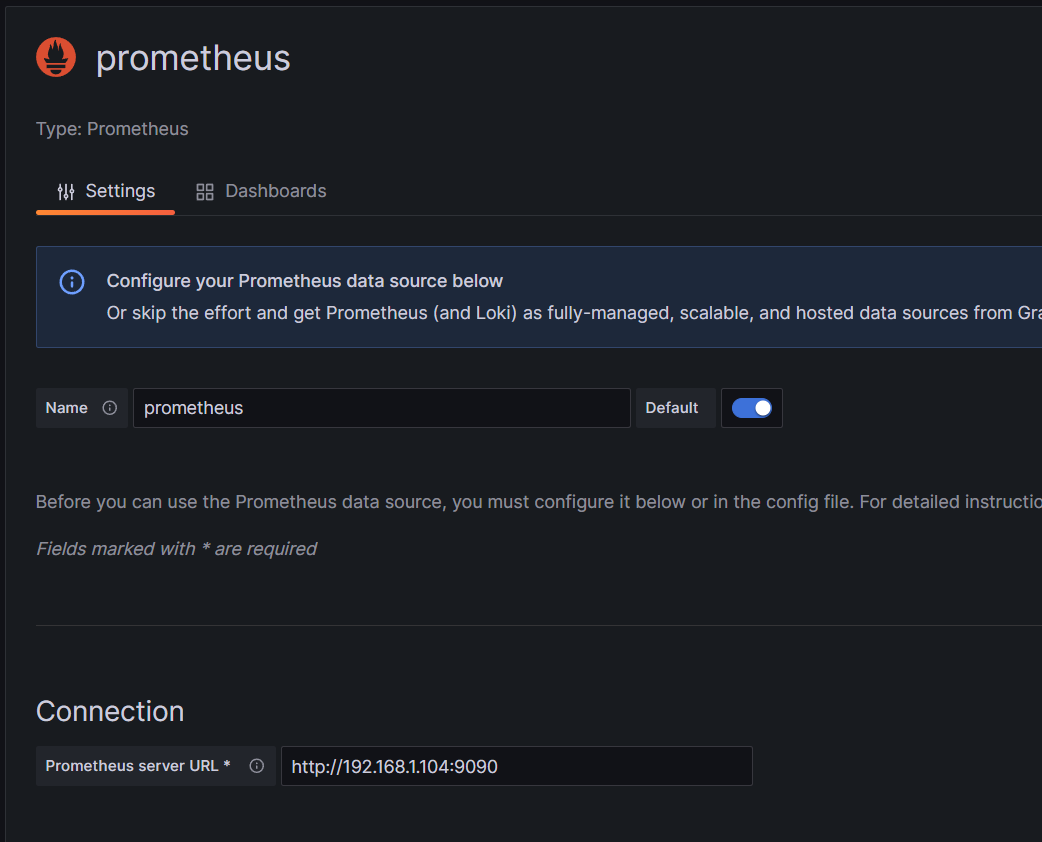
\includegraphics[width=1\linewidth]{prometheusDodanieGrafana.png}
    \caption{Dodanie Prometheusa w Grafanie}
    \label{fig:enter-label}
\end{figure}

Po zapisaniu nowego źródła widać wiadomość sygnalizującą, że połączenie jest skonfigurowane poprawnie.

\begin{figure}[H]
    \centering
    
\includegraphics[width=1\linewidth]{grafanaPoprawnyPrometheus.png}
    \caption{Wiadomość sygnalizująca poprawne skonfigurowanie Prometheusa}
    \label{fig:enter-label}
\end{figure}

Aby zobaczyć zwizualizowane statystyki serwera, mogę stworzyć w Grafanie nowy dashboard i jako źródło podać ID dashboardu stworzonego przez społeczność \lstinline|https://grafana.com/grafana/dashboards/1860-node-exporter-full/|.

Po zapisaniu zmian widzę już zwizualizowane statystyki serwera.

Należy jednak pamiętać, że zrestartowanie kontenera z \textbf{Grafaną} spowoduje utratę zmian. W tym celu użyję takiego samego podejścia, jak w przypadku \textbf{Prometheusa}. Konfigurację \textbf{Grafany} przeniosę do pliku i zamontuję go jako plik konfiguracyjny przy starcie kontenera.

\begin{figure}[H]
    \centering
    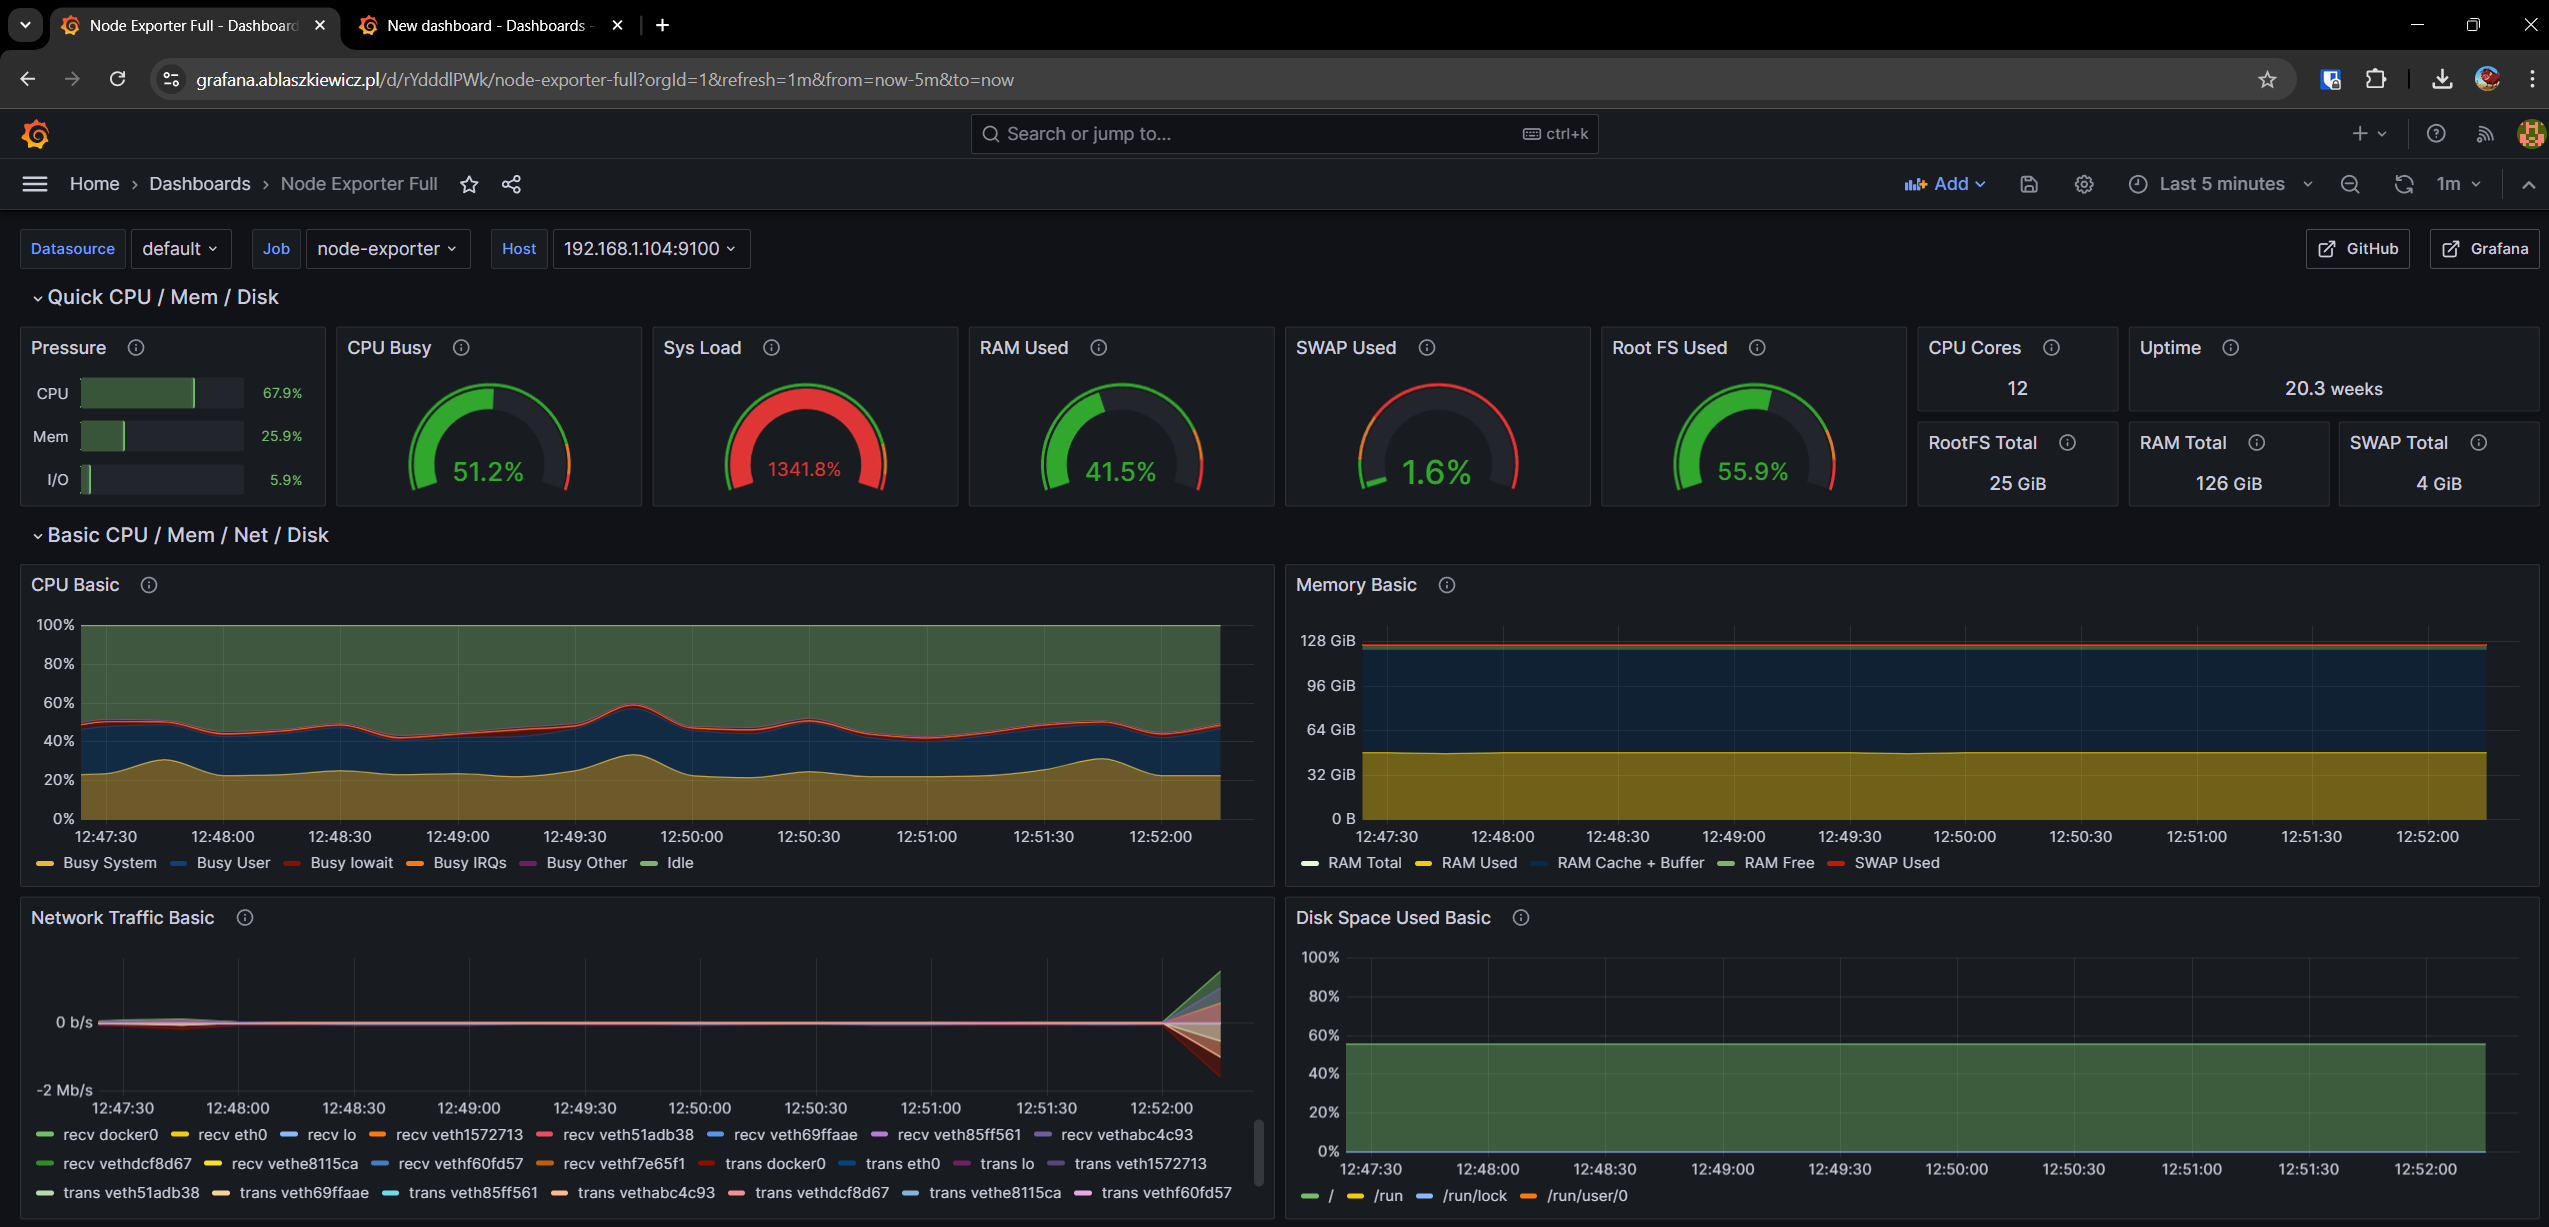
\includegraphics[width=1\linewidth]{grafanaNodeExporterDashboard.png}
    \caption{Dashboard Node Exportera w Grafanie}
    \label{fig:enter-label}
\end{figure}

\begin{lstlisting}[caption=Plik \texttt{infrastructure/grafana/datasources/datasources.yml}]
apiVersion: 1

datasources:
  - name: Prometheus
    type: prometheus
    access: proxy
    uid: prometheus_datasource_uid
    url: http://192.168.1.104:9090
\end{lstlisting}

\begin{lstlisting}[caption=Plik \texttt{infrastructure/grafana/dashboards/dashboards.yml}]
apiVersion: 1

providers:
  - name: dashboards
    type: file
    updateIntervalSeconds: 30
    options:
      path: /etc/grafana/provisioning/dashboards
      foldersFromFilesStructure: true
\end{lstlisting}

Dodatkowo używając UI Grafany wyeksportowałem aktualny dashboard jako JSON i wkleiłem go do \lstinline|infrastructure/grafana/dashboards/node-exporter.json|.

Na koniec zostało zmodyfikować template wdrażający Grafanę tak, aby montował wcześniej stworzone pliki jako volume.

\begin{lstlisting}[caption=Zmodyfikowany plik \texttt{.github/templates/deploy-grafana/action.yml}]
name: Deploy grafana

inputs:
  ssh-host:
    required: true
  ssh-username:
    required: true
  ssh-port:
    required: true
  ssh-key:
    required: true

  grafana-username:
    required: true
  grafana-password:
    required: true

runs:
  using: 'composite'
  steps:
    - name: Deploy grafana
      uses: appleboy/ssh-action@master
      with:
        host: ${{ inputs.ssh-host }}
        USERNAME: ${{ inputs.ssh-username }}
        PORT: ${{ inputs.ssh-port }}
        KEY: ${{ inputs.ssh-key }}
        script: |
          rm -rf ~/provisioning/grafana
          mkdir -p ~/provisioning/grafana
          cd ~/provisioning/grafana
          git clone https://github.com/ablaszkiewicz/devops-sandbox.git
          cd devops-sandbox/infrastructure/grafana


          docker run \
            -d \
            -p 2000:3000 \
            --add-host=host.docker.internal:host-gateway \
            --name=monitoring-grafana \
            -e "GF_INSTALL_PLUGINS=grafana-worldmap-panel" \
            -e "GF_PATHS_PROVISIONING=/etc/grafana/provisioning" \
            -e "GF_SECURITY_ADMIN_USER=${{ inputs.grafana-username }}" \
            -e "GF_SECURITY_ADMIN_PASSWORD=${{ inputs.grafana-password }}" \
            -v $PWD/dashboards:/etc/grafana/provisioning/dashboards \
            -v $PWD/datasources:/etc/grafana/provisioning/datasources \
            --restart=always \
            grafana/grafana:10.3.3
\end{lstlisting}

Dokonałem teraz ponownego wdrożenia kontenera z Grafaną. Po restarcie widzę skonfigurowane źródło danych oraz dashboard.

\subsubsection{Logi nginx}

\subsubsection{Promtail}

\subsubsection{Loki}

\section{Optymalizacje}
\subsection{Cachowanie buildów}
\subsection{Odporność na restarty}



\begin{thebibliography}{9}

\bibitem{flickr}
John Allspaw, Paul Hammond (2009) 10+ Deploys per Day: Dev and Ops Cooperation at Flickr \url{https://www.slideshare.net/jallspaw/10-deploys-per-day-dev-and-ops-cooperation-at-flickr}

\bibitem{devOpsDays}
Strona internetowa DevOpsDays \url{https://devopsdays.org/}

\bibitem{devOpsHandbook}
Gene Kim, Patrick Debois, Professor John Willis, Jez Humble (2016) The DevOPS Handbook: How to Create World-Class Agility, Reliability, and Security in Technology Organizations

\bibitem{damonEdwards}
Damon Edwards (2010) What is DevOps? \url{http://dev2ops.org/2010/02/what-is-devops/}

\bibitem{cdDockerJenkins}
Rafał Leszko (2017) Building CI/CD using Docker and Jenkins

\bibitem{royceWaterfall}
Winston Royce (1970) Managing the Development of Large Software Systems

\end{thebibliography}

\end{document}

